\documentclass[letterpaper,12pt,final,openright,twoside]{memoir}
\RequireXeTeX

\newcommand{\thesisTitle}{Measuring Cultural Transmission at Archaeological Scales:  Machine Learning and Agent-Based Simulation Methods}
\newcommand{\thesisAuthor}{Mark Ernest Madsen}
\newcommand{\authorDegree}{\footnotesize{\textsc{M.S., Anthropology}}}



\usepackage{amsmath}
\usepackage{mathspec}
\makeatletter % undo the wrong changes made by mathspec
\let\RequirePackage\original@RequirePackage
\let\usepackage\RequirePackage
\makeatother

%Date definition
\usepackage{datetime}
\newdateformat{yearonly}{\monthname[\THEMONTH]~\THEYEAR}
\date{\yearonly\today}

\newdateformat{pubyear}{\THEYEAR}

\usepackage[osf]{mathpazo}
\usepackage{fontspec}
%Set fonts

\usepackage{amsfonts}
\usepackage{amssymb}

\usepackage{mathrsfs} % For Cursive Fonts, dont define with mathdesign
\usepackage{lipsum}
\usepackage{xspace}
\usepackage[chapter,ruled]{algorithm}
\usepackage{algorithmic}

\usepackage{boxedminipage}
\usepackage{fancyvrb}
\usepackage{xltxtra}
\usepackage{xunicode}
\defaultfontfeatures{Scale=MatchLowercase}

%Math Fixes
\usepackage{fixmath} %Force ISO math standards
\setmainfont[Ligatures=TeX,Numbers=OldStyle]{Minion Pro}
\setsansfont[Mapping=tex-text]{Ocean Sans Std}
\setmonofont{Bitstream Vera Sans Mono}
\setmathfont(Digits,Latin,Greek)[Script=Math,Uppercase=Italic,Lowercase=Italic]{Minion Math}
\setmathfont[range={\mathbfup->\mathup}]{Minion Math Semibold}
\setmathfont[range={\mathbfit->\mathit}]{Minion Math Semibold}
\setmathfont[range={\mathit->\mathit}]{Minion Math Regular}

\usepackage{varioref} %extends \pageref via \vref to automate things like "on the next page"
\usepackage[xetex,breaklinks,plainpages=false,pdfpagelabels]{hyperref}
\usepackage[]{natbib} %For References
\usepackage{memhfixc} %Allows Hyperref in Memoir
% glossaries MUST be loaded after hyperref...
\usepackage[toc,section=chapter]{glossaries}
\makenoidxglossaries

\usepackage{graphicx}
% \usepackage[draft]{pdfpages}
\usepackage{mdwmath} %Math alignment
\usepackage{mdwtab} 
\usepackage[smaller]{acronym} %acronyms package

% allow more complex list environments
\usepackage[inline]{enumitem}
%\setlist{leftmargin=-1\labelwidth}

\setenumerate[1]{label=\Roman*.}
\setenumerate[2]{label=\Alph*.}
\setenumerate[3]{label=\roman*.}
\setenumerate[4]{label=\alph*.}

\newenvironment{dissparalist}{\begin{enumerate*}[label=(\emph{\alph*}),before=\unskip{: }, itemjoin={{; }}, itemjoin*={{, and }}]}{\end{enumerate*}}
%Version control with GIT
\usepackage[footinfo]{gitinfo}


\newcommand{\pgstyle}{Ruled}

%----------------- preamble.tex -------------------

\hypersetup{colorlinks,citecolor=blue,filecolor=blue,linkcolor=blue,urlcolor=blue}

\maxsecnumdepth{subsubsection} %Number Subsections too

% Redo for letter paper - although this might need further tweaking, it's rough
%\settrimmedsize{279mm}{215mm}{*}
\setlength{\trimtop}{0pt}
\setlength{\trimedge}{\stockwidth}
\addtolength{\trimedge}{-\paperwidth}
%\settypeblocksize{634pt}{440pt}{*}
\settypeblocksize{8.5in}{6.5in}{*}
\setlrmargins{*}{*}{1}
\setulmargins{*}{*}{1}
\setmarginnotes{17pt}{51pt}{\onelineskip}
\setheadfoot{2\onelineskip}{2\onelineskip}
%\setheaderspaces{*}{2\onelineskip}{*}
\setheaderspaces{*}{*}{*}
\setSpacing{1}
\checkandfixthelayout

% Captioning
\changecaptionwidth
\captionwidth{0.925\textwidth}

% Float enabling
\newsubfloat{figure} %Enable subfigures
\pagestyle{\pgstyle}

%--------------- chpstyle.tex

%-----------------Book Style-----------------
\makeheadstyles{thesis}{%
% book changes
\renewcommand*{\booknamefont}{\huge\sffamily\bfseries}
\renewcommand*{\booknumfont}{\huge\sffamily\bfseries}
\renewcommand*{\booktitlefont}{\Huge\sffamily\bfseries}
\renewcommand*{\midbookskip}{\par\vskip 2\onelineskip}%
% part changes
\renewcommand*{\partnamefont}{\huge\bfseries\sffamily}
\renewcommand*{\partnumfont}{\sffamily\bfseries\huge}
\renewcommand*{\parttitlefont}{\Huge\bfseries\sffamily}
\renewcommand*{\midpartskip}{\par\vskip 2\onelineskip}%
%Chapter Style
\chapterstyle{veelo} %Chapter Style Type (see memoir package docs)
\setlength{\beforechapskip}{12mm} %Shorten number
\renewcommand*{\chapnamefont}{\sffamily\bfseries\LARGE\flushright}
\renewcommand*{\chapnumfont}{\sffamily\bfseries\Huge}
\renewcommand*{\chaptitlefont}{\sffamily\HUGE\bfseries\flushright}
% section
\setsecheadstyle{\sffamily\Large\bfseries\raggedright}%
% % subsection
\setsubsecheadstyle{\sffamily\large\bfseries\raggedright}%
% % subsubsection
\setsubsubsecheadstyle{\sffamily\normalsize\bfseries\raggedright}%
% % paragraph
\setparaheadstyle{\normalfont\normalsize\bfseries}%
% % subparagraph
\setsubparaheadstyle{\normalfont\normalsize\bfseries}
}
\usepackage{hyphenat}
\usepackage{subcaption}
\usepackage{rotating}
\usepackage{diss-macros}

\begin{document}





\headstyles{thesis}

\frontmatter %-----------------
\small
\begin{titlingpage}
\mbox{}

\begin{center}

{\large Chapter \ref{chap:semanticaxelrod-paper} \copyright Copyright 2015 \par}

{\large All other materials \copyright Copyright 2020 \par}

 {\large \thesisAuthor\par}%
 
 \vskip 1cm

\includegraphics[scale=0.5]{graphics/by-nc-sa.eps}



\end{center}
 \vfill
\end{titlingpage}



\begin{titlingpage}
\begin{center}\leavevmode
%\begin{flushright}\leavevmode

    \normalfont
    \vfill

    {\Large \textsc{\thesisTitle}\par
    \hrulefill\par}
    
    \vfill
    
    {\Large \thesisAuthor\par}%

	\vfill
    
    {\large \textsc{A dissertation
submitted in partial fulfillment of the
requirements for the degree of Doctor of Philosophy\\[0.5em]}}
    
\vfill

%    \vfill
%    {\Large Draft \par}%
%    \vfill
    
    {\large \textsc{University of Washington\\ 2020}}

	\vfill
	
	{\large \textsc{Reading Committee:}\\
	James K. Feathers, co-Chair\\
	Benjamin Marwick, co-Chair\\ }
	
	\vfill
	
	{\large \textsc{Program Authorized to Offer Degree:}\\
	Anthropology\\}
	
	

%\end{flushright}%
\end{center}%
\end{titlingpage}




%----- Abstract
\begin{titlingpage}
\begin{center}

{\large University of Washington \par}

\vskip 0.75cm

 {\large \textbf{Abstract} \par}%
 
 \vskip 0.75cm
 
    { \thesisTitle\par}
    
    \vskip 0.5cm
  
      { \thesisAuthor\par}%
      
      \vskip 0.5cm
      
      {Co-Chairs of the Supervisory Committee:\\
      Research Associate Professor James K. Feathers\\
	Associate Professor Benjamin Marwick\\
	Anthropology\\}

\end{center}
	
%% Actual abstract goes here
\DoubleSpacing
\noindent Cultural transmission has long been a key organizing principle within anthropology, but the effort to formalize cultural transmission models and fit them to archaeological data is more recent, stimulated by work by Robert Dunnell in the 1970's.  Since then, the use of cultural transmission modeling in archaeology has branched into several research programs:  one macroevolutionary, employing phylogenetic methods; and one microevolutionary, employing models derived from population genetics.  A third research program, focused on intermediate or "mesoscopic" scales and seriation as a finer-grained counterpart to phylogenetic and cladistics, is being developed by Carl Lipo and the present author.  

This dissertation collects research papers by the author since 2012 which examine two questions.  First, are equifinality issues encountered in the microevolutionary research program solvable or do they prevent us from employing individual-scale models?  Second, to the extent that equifinality cannot be circumvented, can we construct better approaches at the mesosopic scale appropriate to coarse grained, time averaged data?

Two papers examine the first question, using simulation modeling and statistical methods to test whether theoretical models can be distinguished even in principle.  The first paper examines the effects of temporal aggregation, which is ubiquitous in the archaeological record, on our ability to distinguish between cultural transmission models, and finds significant issues in doing so with time averaged data.  The second paper examines the effects of population heterogeneity in social learning modes, which is well documented from living human and animal populations.  I find that heterogeneous mixtures of social learning rules can be identified statistically, but only with synchronic censusing of the population, and that time averaging and small samples render mixtures indistinguishable from pure unbiased copying.  

Turning to the second question, three papers continue my long-term research into reshaping the classical seriation method into a tool for tracing the structure of cultural transmision at regional scales.  One short paper examines the combinatorial structure of the seriation problem when we admit multiple subsolutions.  A second paper seeks to increase the size of possible seriations, which is necessary to incorporate significant spatial variation and yield a tool usable for investigating the history of cultural transmission in a region.  We increase the potential size of seriation solutions by switching from unimodality to distance minimization as the ordering criterion, yielding ``continuity'' seriation as a distinct method.  A third paper in this group then applies continuity seriation graphs as the observable variable, in a methodological study of how to construct models of how cultural transmission was structured at the regional scale.  This paper introduces ``interval temporal networks'' as a way to formalize our hypotheses about regional interaction and transmission, and explores a statistical method for summarizing the topology of seriation graphs, to assess their fit to our regional interaction models.

A final paper examines a different kind of mesoscale question:  how do we begin to model not just the spatiotemporal structure of past cultural transmission, but its \emph{content} as well.  The chapter models the dependency structure of the knowledge required to construct complex artifact types, through the ``prerequisites'' needed for each step, and introduces a model where transmission of subsequent traits requires learning their prerequisites first.  This simplified model of ``structured'' cultural traits is then used to explore the ``learning hypothesis'' for behavioral modernity, by looking at the richness and depth of knowledge gained when transmission is mostly accomplished by simple imitation compared to learning via a teacher.  The results are suggestive that the learning hypothesis can account for the increased richness of ``behaviorally modern'' hominids, and more importantly, points the way to more substantive and technologically informed cultural transmission models.  


\end{titlingpage}


\renewcommand{\cftchapterfont}{\normalsize\normalfont}   
\renewcommand{\cftpartfont}{\normalsize\normalfont}   
\renewcommand{\cftsectionfont}{\normalsize\normalfont} 
\renewcommand{\cftsubsectionfont}{\normalsize\normalfont} 
\renewcommand*{\cftpartname}{Part\space}
\newpage
\setcounter{tocdepth}{3} 
%\cftsetindents{chapter}{1.5em}{3.0em}
%\cftsetindents{section}{3em}{3.0em}
%\cftsetindents{subsection}{4.5em}{3.0em}
\tableofcontents*
\cleardoublepage
\listoffigures
\cleardoublepage
\listoftables
\cleardoublepage
% \listofalgorithms

% \listoflistings

%\printnomenclature % Notation stuff in main tex file

\clearpage
\chapter{Acknowledgements}

The University of Washington Department of Anthropology, with whom I have been fortunate to be associated in one form or another since 1985, provided financial support, lab space, computer time (back in the days when you paid by the hour!), and other resources needed to conduct this research.  Most of all, the Department tolerated and supported the unusual and circuitous path my graduate studies and research have taken.  Thank you for your support.  I was introduced to the Department by Stevan Harrell through his participation in the UW Honors Program.  Faculty with whom I had significant interaction and who influenced me include Jim Green, David Spain, Stevan Harrell, Miriam Kahn, Laura Newell, Steven Goodreau, Gerald Eck, Eric Alden Smith, Julie K. Stein, Donald K. Grayson and Robert Wenke.  Thank you all for a superb education.  I also wish to thank Peter D. Ward, whose graduate paleobiology course in the spring quarter of 1987 substantially increased my understanding of evolutionary biology and broadened my research horizons.  

\vskip 0.3cm

I thank everyone who has served on both incarnations of my dissertation committee, including Robert C. Dunnell, Donald K. Grayson, Thomas Stoebe, Carl Bergstrom, Carl Lipo, Ben Marwick, and James K. Feathers.  In particular, Jim Feathers and Ben Marwick provided strong encouragement at a key moment, and my gratitude for that push is eternal.  Thank you both.

\vskip 0.3cm

Carl Lipo has been a friend, colleague, and much more since 1988.  Our collaboration is strongly represented in these pages, and I look forward to many more years of thinking about these issues and collaborative work together.  

\vskip 0.3cm

Over the years, my colleagues from the Department have become friends, many lifelong and beyond.  I want to specifically thank Sarah Sterling, Fran Hamilton, Michael Pfeffer, Betsy Scharf, Steve Cole, and Chris Pierce.  Most especially, Kim Kornbacher left us before I could finish this and share the joy with her, but she lives forever in my heart.  Kris Wilhelmsen---please know that you and Kim are forever family to me!

\vskip 0.3cm

A very special thanks goes to Lara Braithwaite, life partner and friend, for sustaining me through the latter stages of this project with great love, encouragement, and steadfast support.  Thank you for our life together! 
\vskip 0.3cm

Finally, I thank Robert Chester Dunnell for the gift of his teaching, his thought, his insatiable curiosity, and his discipline.  Dr. Dunnell was the very model of a scientist and scholar, and his influence can be seen on every page.  From the moment I walked into his Archy 497 classroom in the autumn of 1986, he has been an inspiration, and set a standard to which I continue to try to attain.  








\newpage
\thispagestyle{empty}
\vfill
%\Centering
\begin{center}
\begin{minipage}[h]{\textwidth}
 \begin{center}
  \vspace{8cm}
  \vfill
  \textit{My mother, Joy Colleen Berkey Madsen (1944-2005),  encouraged me from the earliest age in a love of learning, not merely because it would lead to opportunity, but because knowledge and learning were important values in and of themselves.  Her own  opportunities for higher education were limited by the need to support herself from a young age, and then by the need to work and support her family, but she supported my education in every way possible.}\\
  \vspace{1cm}
  \textit{This dissertation is both dedicated to her, and many ways a joint accomplishment.}
  \vfill
 \end{center}
\end{minipage}
\end{center}
%\justifying

% \newpage 

% 

\setcounter{page}{0} %Suppresses Hyperref errors on ``Same Identifier''
\newpage
\thispagestyle{empty}

\renewcommand{\epigraphflush}{center} % centered epigraph env
\renewcommand{\epigraphsize}{\large} %larger font
\renewcommand{\textflush}{center} % Centered text
\setlength{\epigraphwidth}{0.7\textwidth} % Wider env

%\epigraph{\vspace{8.55cm}``Computing Science is no more about computers than Astronomy is about telescopes.''}{\Dijkstra}


\epigraph{\vspace{1cm}``There are really only individuals in nature\ldots genera, orders, and classes exist only in our imagination.''}{Georges-Louis Buffon, \emph{Histoire Naturelle}, Volume 1, 1749--1804}


\epigraph{\vspace{1cm}``We cannot improve the language of any science without at the same time improving the science itself.\ldots Neither can we, on the other hand, improve a science, without improving the language or nomenclature which belongs to it.''}{Antoine Lavoisier, \emph{Elements of Chemistry}, 1789}



\epigraph{\vspace{1cm}``It is not always appreciated that the problem of theory building is a constant interaction between constructing laws and finding an appropriate set of descriptive state variables [units] such that laws can be constructed.  We cannot go out and describe the world in any old way we please and then sit back and demand that an explanatory and predictive theory be built on that description \ldots That is not to say that there is an insoluable contradiction. Rather there is a process of trial and synthesis going on in which both state descriptions and laws are being fitted together\ldots''}{\Lewontin, \citeyearpar{Lewontin1974}}




\renewcommand{\epigraphflush}{flushright}
\renewcommand{\epigraphsize}{\small}
\setlength{\epigraphwidth}{0.4\textwidth}
\renewcommand{\textflush}{flushleft}



\newpage
%\input{content/preface}

\mainmatter %-----------------
\normalsize
\acresetall    %Reset acronyms

\DoubleSpacing
%%%%%%%%% Content %%%%%%%%%%%%

\part{Introduction and Research Methods}
\addtocontents{toc}{\protect\mbox{}\protect\hrulefill\par}
\label{part:intro}

    \chapter{Introduction}
    \label{chap:intro}
    % \begin{description}[leftmargin=-1\labelwidth]
% \item[\textsc{Overview}] \lipsum[1]
% \end{description}

From our vantage point in 2019, it seems as if the study of cultural transmission is a  formalized, model-driven, highly interdisciplinary field, encompassing the “hard science” side of most of the traditional social sciences including psychology, economics, parts of cognitive science, sociology, anthropology, a strong representation among the behavioral aspects of evolutionary biology and zoology, and an increasing number of physicists who have turned their mathematical and modeling talents away from the realm of the very tiny to the realm of the relational and social.  Indeed, at this point it seems as if anthropology and especially the sub-discipline of archaeology are followers and consumers of cultural transmission theory, not leaders in its development and application.  And yet anthropology is the only discipline of those named in which cultural transmission is — and has been, for more than a century — a \emph{central organizing concept} for the discipline \citep{Lyman1998}.  Why are we perceived as followers, even sometimes by ourselves?  

Part of the answer lies in the qualitative and descriptive heritage of anthropology and archaeology; until recently we imported much of our quantitative theory from outside the discipline, using it to form narratives, and still are heavy borrowers.  But I will argue in this work that part of the answer lies in a scale distinction between much of the individual-level work on cultural transmission theory and the phenomena that anthropology has traditionally dealt with — and that archaeology still does, of necessity.  That scale distinction is holding us back, unless we address it.

The phenomena we seek to explain in archaeology are always aggregate in nature, always time-averaged records of many events of occupation and activity.  Ours is an observational science, not an experimental or laboratory discipline, and we are not in full control of the time spans over which the deposits we collect and excavate, and the “assemblages” that result from those collections, possess.  Although there is a robust community within archaeology working on problems that involve cultural transmission models and their predictions, ours is not an empirical record which informs on transmission chains and individual-level cognitive biases.  Ours is an empirical record of past behavior and cultural evolution that requires coarser-grained theory and models which deal in predictions about aggregate measures of the flow of cultural information and traits over broad spans of geography and history.

On some level, we know this, which is why the archaeological literature on cultural transmission theory and its applications has turned, after a period of “polemic and prototypes”, to attempts to address the equifinalities that result from aggregation and time averaging on our ability to fit the commonly discussed cultural transmission models to archaeological data.  This recent work addresses the dynamic and empirical sufficiency of cultural transmission models in archaeology \citep{Lewontin1974}.  My own early work in this field straddles the line between “polemic and prototypes” and addressing these equifinalities (e.g., \citep{Lipo1997}; REFS).    

Much of the recent work on addressing empirical sufficiency is quite valuable, and along the way I will point out those studies by others which are particularly important for workers in the field who are attempting to solve substantive issues and apply cultural transmission theory.  But it is my central contention that archaeology will continue to be a “borrower” of theory, plagued by issues of equifinality and empirical sufficiency, so long as we continue to attempt to use “observables” — units and variables — which are derived largely from synchronic models and individual-level theories of cultural transmission.  My own recent work is aimed at evaluating the potential for “coarse graining” cultural transmission models to archaeological scales, which means first and foremost, forming a new set of “observable” units which are appropriate to the diachronic, aggregated, and time averaged empirical record we study.  This dissertation is a progress report on forming such observables and examining how to use them to study the kind of data we \emph{actually have}, not the data that would make our task easier — or in other words, the data we \emph{wish} we had.  





\section{The Place of Cultural Transmission Theory in Archaeology}
\label{sec:place-ct-in-archy}

Go through Lyman 2008 summary, importance to evolutionary archaeology but mention that one need not have a strict focus on Darwinian theory to find CT useful, one's ultimate research questions may lie in other areas, but the strong focus on spatiotemporal diffusion, adoption and innovation that cultural transmission theory brings are useful throughout the discipline.  





\section{What is Unique About Studying \CT in Archaeology?}
\label{sec:ct-archy-different}



\section{What Tools Do We Need To Study Past \CT?}
\label{sec:ct-archy-questions}



\section{Research Strategy}
\label{sec:research-strategy}



As previously noted, fully connecting the results of cultural transmission modeling to regional scale seriation algorithms has not been done in the published literature.  Multiple authors \citep[e.g.][]{Lipo1997,Neiman1990,Neiman1995,shepardson2006} have noted that the temporal traces of cultural transmission models often produce seriation-like curves of trait frequency, 

TODO:
Britton Shepardson -- prob need to move this stuff to seriation chapter, discuss unimodality and other criteria there.  here just mention the heuristic stuff like Neiman and Shepherson noting the gross similirity between traces of CT models and seriation curves.



\section{Summary}
\label{sec:plan-of-book}

The outline of the dissertation is as follows. Chapter \ref{chap:historical-perspective} lorem ipsum, sic dolor amet.  

\lipsum[3]






    
    \chapter{Research Methods}
    \label{chap:methods}
    \begin{description}[leftmargin=-1\labelwidth]
\item[\textsc{Overview}] \lipsum[1]
\item[\textsc{Contents}] \lipsum[2]
\end{description}





\part{Research Papers}
\addtocontents{toc}{\protect\mbox{}\protect\hrulefill\par}
\label{part:papers}

    \chapter{Neutral Cultural Transmission in Time Averaged Archaeological Assemblages}
    \label{chap:timeaveraging-paper}
    \begin{description}[leftmargin=-1\labelwidth]
\item[\textsc{Overview}] Neutral models are foundational in the archaeological study of cultural transmission.  Applications have assumed that archaeological data represent synchronic samples, despite the accretional nature of the archaeological record.  Using numerical simulations, I document the circumstances under which time-averaging alters the distribution of model predictions.  Richness is inflated in long-duration assemblages, and evenness is ``flattened'' compared to unaveraged samples.  Tests of neutrality, employed to differentiate between biased and unbiased models, suffer serious problems with Type I error under time-averaging.  Estimation of population-level innovation rates, which feature in many archaeological applications, are biased even without \timeav, but have sharply increased bias given longer assemblage durations.  Finally, the time scale over which time averaging alters predictions is determined by the mean trait lifetime, providing a way to evaluate the impact of these effects upon archaeological samples.
\end{description}


\section{Introduction}\label{ta:sec:introduction}
 
The evolutionary study of culture today crosses many disciplines and employs a variety of experimental and observational methods to study its subject matter.  What makes the archaeological record unique as a source of data concerning the evolution of culture is time depth, creating the possibility of studying both the unique histories of human groups and the evolutionary processes that shape those histories.  Archaeology is not unique in studying temporal data on human activity, but like our colleagues in paleobiology, we study an empirical record that is unlike the time-series data available to disciplines such as economics or epidemiology \citep[e.g.,][]{arrow2009some,keeling2005implications,keeling2007modeling,kendall1953analysis,rothman2008modern}. The archaeological record is not a sample of measurements from individual moments in time stacked together into a sequence.  Instead, archaeological deposits are almost always accretional palimpsests, representing cumulative artifact discard over durations of varying length \citep{bailey2007time,bailey1981concepts,binford1981behavioral,8981,stein1987deposits}.  Thus, when archaeologists count the richness of faunal taxa in an assemblage, or measure the relative frequencies of ceramic types, the data obtained summarize the bulk properties of artifact discard and deposition over significant spans of time, often with nonconstant rates of accumulation.\footnote{As well as the action of various post-depositional and taphonomic processes, of course.}  We refer to assemblages which are accretional in this manner as ``\timeavd.''  

A growing number of studies apply \ct models to artifact assemblages by comparing the predictions such models make for the richness, diversity, or frequency distribution of cultural traits, to counts or frequencies of artifact classes \citep[e.g.,][]{Bentley2003,bettinger1999point,Eerkens2007,8994,Lipo2000,perreault2010mobility,premo2011spatial,scholnick2010apprenticeship,Shennan2001ceramic,shennan2011descent,steele2010ceramic}.  The question is, are model predictions comparable to archaeological measurements?  Given the \timeavd structure of most archaeological deposits, I suspect the answer is no.  Transmission models developed outside archaeology are typically constructed to make predictions concerning variables observed at a point in time.  To date, almost none of the archaeological literature employing \ct models has taken this ``\timeav'' effect into account and modified the way predictions are made to match the nature of the phenomena we measure \citep[cf.][]{bentley2004random}.  Evaluating the effects of temporal aggregation upon the predictions made by \ct models is the first step in understanding how to rewrite and adapt transmission models to understand their dynamics given \timeavd observations.  

In his dissertation, \citet{Neiman1990} considered a potential source of \timeav effects in diachronic assemblages:  variation in discard rates across traits.   With respect to this particular effect within accretional deposits, Neiman's results suggested that the predictions made by a neutral model of \ct were directly applicable to the relative frequencies of traits as we would measure them in a \timeavd assemblage.  Nevertheless, there is good reason to consider the effects of aggregation directly, outside of variation in discard rates.   
Paleobiologists, for example, have documented systematic differences between living and fossil assemblages, including increased species richness, reduced spatiotemporal variance in taxonomic composition, and flatter species abundance curves in \timeavd assemblages \citep{olszewski2011remembrance,tomasovych2010effects,tomasovych2010predicting}.  \citet{lyman2003influence} extended these results to zooarchaeology, noting that \timeav can be a significant problem when the process one is applying or studying occurs over a shorter time scale than the empirical record available to study its properties \citep[see also][]{Grayson1998}.  This relation between time scales is applicable to \ct modeling as well.  

Archaeologists now employ a variety of \ct models, which differ in the kind of variation and traits they describe and the copying rules and evolutionary processes they incorporate.  Discrete models describe individual variants or traits by their count or frequency in a population and are foundational for the study of stylistic variation in many artifact categories (e.g., pottery).  The simplest discrete  model is random copying in a well-mixed population with innovation, representing neutral variation with the stochastic effects of drift.  We frequently construct more complex models of transmission bias by adding additional terms or frequency-dependent copying rates to the basic unbiased copying model \citep{cavalli1973cultural,cavalli1973models,CF1981,BR1985}.  Thus, an understanding of the effects of \timeav upon neutral transmission will be informative about many (if not all) of the discrete transmission models in use by archaeologists today, and forms the focus of the present study.  

I report the results of numerical simulations designed to observe neutral transmission using variables employed in the archaeological literature, aggregated over time at a variety of intervals designed to mimic a wide range of ``assemblage durations.''  In Section \ref{ta:sec:concept-review} I describe the relationship between neutrality, unbiased copying, and the separate but related concept of ``drift,'' followed by a review of the quantitative properties of the well-mixed neutral Wright-Fisher infinite-alleles model in Section \ref{ta:sec:wf-model}.  Section \ref{ta:sec:methods} outlines the simulation model employed to study \timeav in this paper, including model verification and testing, and the algorithm used to effect temporal aggregation within the simulations.  Section \ref{ta:sec:results} presents the results of simulating unbiased \ct for a variety of innovation rates and assemblage durations, and Section \ref{ta:sec:conclusions} summarizes the effects seen and points to next steps in reformulating our \ct models for archaeological contexts.  


\section{Conceptual Structure of Neutral Cultural Transmission}
\label{ta:sec:concept-review}

In his classic article “Style and Function: A Fundamental Dichotomy,” Dunnell \citeyearpar{8961} proposed that many aspects of an artifact would play little or no role in its engineering performance, and thus have no impact on the fitness of individuals employing it. In other words, some attributes of artifacts are neutral with respect to selection.  This has been widely misinterpreted as a claim that the artifacts themselves are neutral or have no fitness value, which is not the case. Dunnell was saying that if one describes an artifact solely using attributes which have equal cost or performance, the resulting classes meet the definition of neutral variation.  

Fraser Neiman \citeyearpar{Neiman1990} first connected Dunnell's identification of style as selectively neutral variation, to population genetic models designed to describe genetic drift.  His dissertation considers a wide range of \ct models, especially those described by \citet{cavalli1973cultural,cavalli1973models,CF1981} and \citet{BR1985}.  Neiman employed simulation to calculate the consequences of both individual processes as well as processes combined with various archaeological factors such as variable rates of artifact discard.  In this work, Neiman pioneered virtually every technique used by archaeologists today to model and study cultural transmission.  The discipline as a whole was introduced to this work in his now classic 1995 article \citep{Neiman1995}, in which the dynamics of Woodland ceramic variation were explicitly modeled as a random copying process.  


Despite the fact that there are multiple ways that neutrality can arise as a population level effect, there is a tendency today to equate neutrality with ``drift'' in the archaeological literature on \ct.   For example, \citet[][p.1443]{bentley2004random} offer a fairly typical description of unbiased \ct as  ``random genetic drift, which describes how the diversity of variants evolve when the dominant process is one of random copying.''  In fact, drift and the copying rules that create population-level trait distributions are different and independent aspects of a transmission system.   Before we turn to the details of a formal model for unbiased, neutral transmission, it is worth reviewing the conceptual elements that make up such models.  


Drift is a feature of any stochastic transmission model in a finite population, regardless of whether selection or bias is also present in the model.   Sewall Wright gave the name ``genetic drift'' to the random fluctuations in gene frequency that occurred because some individuals might be the source of many genes in the next generation, and others none at all.  Translated into a cultural model, drift occurs when some individuals, by random chance, are imitated or copied and others are not.  In an infinite population, by contrast, the variants held by individuals would be sampled at their exact frequencies in the population, and thus there would be no stochastic ``wiggle'' in trait frequencies.  This is reflected in population genetics by the famous ``Hardy-Weinberg'' equilibrium, where in the absence of selection or other forces, gene frequencies stay the same from generation to generation.    This means that we can easily have \emph{neutrality without drift}, in an infinite population.  In a large but still finite population, we can expect drift to have very tiny, potentially even unmeasurable effects upon the trajectory of trait frequencies.   

Drift, moreover, occurs in combination with a variety of inheritance rules, mutation models, and in combination with natural selection.  In small populations, we can expect drift to be a factor when examining the engineering properties of ceramics and the relative fitness of firing technologies, or the fitness of foraging strategies.  Whenever such traits are learned and passed on within small, finite populations, the stochastic aspect of who learns from whom will create fluctuations in variant frequencies that have nothing to do with the performance or survival value of traits, or the prestige of those we choose to learn from or imitate.  In other words, we can have \emph{drift without neutrality}.  In small enough populations or during bottlenecks, even adaptive technologies and knowledge can be lost to drift \citep{8921,henrich2006understanding}.  We should always be on the lookout for the effects of drift, especially as population sizes get smaller as we go back in time.  Drift is not a model of human social learning; it is a consequence of finite populations, injecting stochastic noise into the dynamics of a system that affects our ability to cleanly fit models and test hypotheses.  

Neutrality, by contrast, is a population level phenomenon, arising when there is no net force systematically favoring certain variants over others for a particular dimension of variation.  Most commonly, of course, we mean that there is no natural selection that favors some alleles over others, but from a mathematical perspective, the transmission bias rules of  \citet{CF1981} and \citet{BR1985} are equivalent to selection models.\footnote{In this paper I leave aside the relationship between ``natural'' and ``cultural'' selection, and transmission biases, since such issues are largely philosophical and theoretical and do not affect the nature of the models we employ for quantitative analysis of cultural variation.}   The simplest way for neutrality to arise is for individual social learning to be ``unbiased.''  Unbiased transmission models always yield population-level neutrality for the traits being passed, because the probability of imitating any specific trait is simply proportional to its frequency among individuals in the population.  The Wright-Fisher model is one of the earliest stochastic models in population genetics \citep{provine1989sewall,provine2001origins,wright1931evolution}, and was originally created to describe the process of genetic drift and its effects in combination with other evolutionary processes.  Following Kimura's theory of neutral alleles, Wright-Fisher is also used to describe the evolution of populations in which variants are selectively neutral.  Elaborations of the basic Wright-Fisher model add mutation, selection, loci with multiple alleles, and multiple loci with interactions between loci \citep[see esp.][]{crow1970introduction,Ewens2004}.\footnote{And, the Moran family of models mirrors the Wright-Fisher models, with overlapping generations, by representing dynamics as continuous-time stochastic processes.  Moran models are likely the best framework for modeling \ct when the exact temporal dynamics matters.  In this paper I follow archaeological convention by employing the more familiar Wright-Fisher discrete generation framework.}
 
But unbiased copying is not the only source of neutrality among variants, and it is important to keep this in mind when selecting models to test as explanations for archaeological phenomena.   In any realistic human population, there will be heterogeneity in social learning rules, with individuals using different rules for different traits, or kinds of traits, and perhaps having individual propensities for conformism (all other things being equal) or pro-novelty bias \citep{Mesoudi2009}.  A population which is heterogeneous for such rules may display the characteristic frequency distributions of conformity or pro-novelty biased if we are able to observe small numbers of transmission events or individual transmission chains, while simultaneously cancelling each other out at the level of the population.  In other words, heterogeneity is a major source of equifinality between different models of social learning, when observed through population-level trait frequencies.   No archaeological applications of \ct models today have employed heterogeneous models, probably because the theory behind such models is not well-studied.  But this is clearly a frontier for future research since homogenous models poorly reflect what occurs in real human populations.  

Returning to unbiased models of transmission, we face a further choice in selecting a specific model to employ or study.  In addition to the copying rules, we must specify an innovation rule.  Such a rule answers questions like:  how do new variants enter the population, can variants be invented multiple times independently, and is there a constrained range of variation for a particular dimension of an artifact?  For example, painted design elements on a ceramic pot offer a ``design space'' of possibilities that is potentially unbounded, even if only a tiny fraction of possible designs occur in any archaeological context.  Such attributes are best modeled by the ``infinite allleles'' innovation model.  In contrast, stylistic aspects of lithic tools may be sharply constrained by the technology and materials themselves, and may be best modeled by innovation among a small set of variants, with the material constraints causing frequent ``reinvention'' of the same shapes over and over.   Such attributes are best modeled by constraining the design space, and employing a finite or ``k-alleles'' version of the unbiased model.   Since Neiman's pioneering work, most archaeological applications of neutral models have employed the ``infinite alleles'' variant of the Wright Fisher model  (WF-IA)\citep{kimura1964number}.  Therefore, in the remainder of this paper, I focus on the unbounded model of neutral evolution with innovation, since it is relevant to a large number of archaeological contexts and artifact categories, but the reader should be aware that the models with a constrained number of variants may be hugely important in specific archaeological contexts, and are underexplored in the archaeological literature.  

\section{Unbiased Transmission:  The Wright-Fisher Infinite-Alleles Model}
\label{ta:sec:wf-model}

WF-IA is a stochastic process that models unbiased transmission within a fixed-size population as multinomial sampling with replacement, with a mutation process that adds new variants to the population at a known rate.  After describing the model, I review the sampling theory of \citet{ewens1972sampling}, which gives the distribution of variants expected in small samples taken from the population as a whole.  The sampling theory, rather than the distribution of variants in the full population, is both well-understood, and most relevant to archaeologists, who are always sampling an empirical record of past artifact variation.

The well-mixed neutral Wright-Fisher infinite-alleles model \citep{kimura1964number} considers a single dimension of variation (``locus'') at which an unlimited number of variants (``alleles'') can occur, in a population of $N$ individuals.\footnote{Conventionally, the model treats a diploid population, in which N individuals each have two chromosomes and thus there are always 2N genes tracked in the population.  The haploid version is more appropriate for modeling cultural phenomena, and thus formulas given in this paper may differ from those given by \citet{Ewens2004} and other sources by a factor of two.  For example, the key parameter $\theta$ is defined as $2N\mu$ rather than the common genetic definition $4N\mu$.}  The state of the population in any generation is given in several ways:  a vector representing the trait possessed by each individual (census), a vector giving the abundance of each trait in the population (occupation numbers), or by the number of traits represented in a population by a specific count (spectrum).  

In each generation, each of $N$ individuals selects an individual at random in the population (without respect to spatial or social structure, hence ``well-mixed''), and adopts the trait that individual possessed in the previous generation.\footnote{An individual can select themselves at random since sampling is with replacement, and this would be equivalent to ``keeping'' one's existing trait for that generation.}  Equivalently, a new set of $N$ individuals are formed by sampling the previous generation with replacement.  At rate $\mu$ for each individual, a new variant is added to the population instead of copying a random individual, leading to a population rate of innovations $\theta = 2N\mu$ \citep{Ewens2004}, with no ``back-mutation'' to existing traits.\footnote{It is important to note that $\theta$ is not a measure of the ``diversity'' of traits in the population, as it has been employed in several archaeological studies, but is instead a \emph{rate} parameter of the model.}  An important consequence of this innovation model is that each variant is eventually lost from the population given enough time, and replaced with new variants.  Thus, there is no strict stationary distribution for the Markov chain describing WF-IA, although there is a quasi-stationary equilibrium in which the population displays a characteristic number of variants, with a stable frequency distribution governed by the value of $\theta$ \citep{Ewens2004,watterson1976stationary}.   

Beginning with a now-classic paper \citet{ewens1972sampling} constructed a sampling theory for the neutral WF-IA model, allowing the calculation of expected moments and frequency distributions for small samples (compared to overall population size) \citep[see ][for a complete summary of results on the sampling theory]{Ewens2004}.  In what follows, we assume that a neutral WF-IA process is running within a population of size $N$.  At some moment in time after the population has reached its quasi-stationary equilibrium, we take a sample of $n$ individuals, where the sample is small compared to the population size ($n \ll N$).  We then identify the variants held by each individual.  The total number of variants seen in the sample will be denoted by $k$, or $k_{\text{obs}}$ depending upon context.     

Given such a sample, \citet{ewens1972sampling} found that the joint distribution of the variant spectrum ($a_i$ represents the number of variants represented $i$ times in a sample), given the population innovation rate ($\theta$), is given by the following formula (now known as the Ewens Sampling Distribution):

\begin{equation}
\label{eq:esd}
\mathbb{P}_{\theta,n}(a_i, \ldots, a_n) = \frac{n!}{\theta^{(n)}} \prod^n_{j=1} \frac{(\theta/j)^{a_j}}{a_j!}
\end{equation}

where $\theta^{(n)}$ is the Pochhammer symbol or ``rising factorial'' $\theta(\theta+1)(\theta + 2)\cdots(\theta + n - 1)$.  In most empirical cases, we cannot measure (or do not set through experiment) the value of $\theta$, so a more useful relation is the distribution of individuals across variants (i.e., the occupation numbers), conditional upon the number of variants $k_{\text{obs}}$ observed in a sample of size $n$:

\begin{equation}
\label{eq:conditional-esd}
\mathbb{P}(n_1, n_2, \ldots, n_k | k_{obs}) = \frac{n!}{|S^k_n| k! n_1 n_2 \cdots n_k}
\end{equation}

where $|S^k_n|$ denote the \emph{Stirling numbers of the first kind}, which give the number of permutations of $n$ elements into $k$ non-empty subsets \citep{abramowitz1965}.  The latter serves here as the normalization factor, giving us a proper probability distribution.   

From Ewens's sampling theory, and in particular Equation \ref{eq:conditional-esd}, a number of useful measures can be derived, relevant to archaeological applications.  In this study, I focus upon the most commonly used:  statistical tests of neutrality, estimation of innovation rates ($\theta$), and the evenness with which variants are represented in the population (as revealed by several diversity measures).  

\subsection{Statistical Tests for Neutrality}
\label{ta:sec:neutrality-test}

Because Equation \eqref{eq:conditional-esd} requires no unobservable parameters, it serves as the basis for goodness-of-fit tests between empirical samples and the neutral WF-IA.  The two most important such tests are the Ewens-Watterson test using the sample homozygosity and Slatkin's ``exact'' test \citep{durrett2008,Ewens2004,slatkin1994exact,slatkin1996correction,slatkin1994exact,slatkin1996correction}.\footnote{There are several other important tests of neutrality when dealing with DNA sequence data, including Tajima's D, the HKA test, and the McDonald-Kreitman test \citep{durrett2008}.  Because their assumptions are highly specific to the structure of sequence data, I omit consideration of them here.}  Both have been adopted for use by archaeologists, beginning with \citet{Neiman1995} and \citet{Lipo2001b}, who described Watterson's work in detail, and more recently, applications of Slatkin's exact test by \citet{steele2010ceramic} and \citet{premo2011spatial}. 

The Slatkin test makes no assumptions concerning the process underlying an alternative hypothesis to neutrality, whereas the Ewens-Watterson test examines the observed heterozygosity at a locus versus the expected heterozygosity predicted by Ewens sampling theory.  Slatkin's test does not employ the concept of heterozygosity, and relies only upon the ``shape'' of the Ewens Samping Distribution given a specific innovation rate.  As a result, archaeologists should prefer Slatkin's test for examining the fit of a synchronic sample of variants to the null hypothesis of neutrality.  Slatkin's test is modeled upon the Fisher exact test for contingency tables.  Where the Fisher exact test determines the probability of an unordered configuration from the hypergeometric distribution, Slatkin's test determines the probability of a sample of traits (characterized by occupation numbers) with respect to Equation \ref{eq:conditional-esd}.  

There are two methods for determining how probable a given sample is, with respect to the ESD.  For relatively small $n$ and $k$, it is possible to enumerate all possible combinations ($\mathbf{C}$) of the $n$ individuals among $k$ variants.  Each configuration ($c_j \: \in \: \mathbf{C}$) then has a probability given Equation \ref{eq:conditional-esd}, as does the observed configuration ($c_{\text{obs}}$).   With larger sample sizes and values of $K_{\text{obs}}$, it becomes impractical or simply time consuming to enumerate all possible configurations and thus determine the likelihood of an observed sample.  In such cases, Monte Carlo sampling of configurations from the Ewens Sampling Distribution is used.  We then determine the total probability mass of all configurations (enumerated or sampled) whose probability are less than or equal to the observed configuration:

\begin{equation}
\label{eq:slatkin-pe}
\mathbb{P}_e = \sum_{c_j \in \lbrace \mathbf{C} \: : \:  P(c_j \: | \: k) \; \leq \; P(c_o \: | \: k)\rbrace} \mathbb{P}(c_j \: | \: k)
\end{equation}

$\mathbb{P}_e$ then represents the Fisherian p-value of the sample with respect to the Ewens Sampling Formula, and thus can be interpreted as a test of the hypothesis that the sample was drawn from a neutral dimension of variation which followed the WF-IA copying model.  The $\mathbb{P}_e$ value for a given sample gives the tail probability of its occurrence given the ESD.  Thus, if we take a sample of size 100 in a population with innovation rate $\theta =  0.1$, and identify two variants with counts 51 and 49, we might not be surprised to see a $\mathbb{P}_e$ value of 0.01181, indicating that such a sample is highly unusual for a WF-IA process.  On the other hand, in the same sample of size 100, if we identify four variants, with counts 55, 38, 6, and 1, this seems a much more typical result of an unbiased copying process.  Indeed, the $\mathbb{P}_e$ value of 0.48544 confirms that we should expect to see such samples quite often. 


\subsection{Estimation of Innovation Rates}
\label{ta:sec:theta-estimation-theory}

The behavior of the WF-IA neutral model is governed by the innovation rate ($\theta$).  Recall that $\theta = 2 N \mu$, and thus represents the population-level rate at which new variants enter the population.  In general, for low values of the innovation rate ($\theta < 1.0$), the process is ``drift-dominated,'' and one or a small number of variants dominate the population.  At innovation rates above 1.0, which implies that every single ``generation'' incorporates one or more new variants, the process is ``mutation-dominated,'' and more variants are maintained at intermediate frequencies in the population.  

Thus, estimation of the innovation rate from empirical data is of great interest when investigating empirical cases.   If we measure the number of variants ($K_n$) in a sample of artifacts of size $n$, the sampling theory  gives the following probability distribution \citep[Eq. 3.84]{Ewens2004}:

\begin{equation} 
\label{eq:full-distro-kn}
	\mathbb{P}_{\theta}(K_n = k) = \frac{|S^k_n| \theta^k}{\theta^{(n)}}
\end{equation}

This is a somewhat inconvenient distribution to work with directly, since calculating the Stirling numbers and rising factorials is both analytically difficult and computationally expensive, but the expected value of $K_n$ has a simple form:

\begin{equation} 
\label{eq:expected-kn}
	\mathbb{E}(K_n) = \frac{\theta}{\theta} + \frac{\theta}{\theta + 1} + \frac{\theta}{\theta + 2} + \cdots + \frac{\theta}{\theta + n - 1}
\end{equation}

$K_n$ is the sufficient statistic for $\theta$, containing all of the information required to calculate the maximum likelihood estimate of the innovation rate ($\hat{\theta}$) from an empirical sample.  This is done numerically by finding the value of $\theta$ that maximizes the likelihood function of Equation \ref{eq:full-distro-kn}, or equivalently, finding the value of $\theta$ for which the expected value of $K_n$ given Equation \ref{eq:expected-kn} is equal to the observed number of variants in a sample (since the full distribution may not have a closed-form likelihood function).  In the archaeological literature, \citet{Neiman1995} introduced this estimator of $\theta$ and called it $t_e$.  With larger samples, \citet{watterson1975number} showed that $k\;/\;\log n$ is a good approximation for the MLE estimator \citep{durrett2008}.  

Despite the fact that this estimator (and its approximations) are the best that can be achieved from samples, \citet{ewens1972sampling} showed that all such estimates of $\theta$ are biased.  Simulations demonstrate, furthermore, that $\hat{\theta}$ (or $t_e$) is an overestimate of the actual value, and that the amount of bias increases with $\theta$ itself \citep{ewens1974some}.   In addition, the variance of the estimator is quite large, and decreases very slowly with increased sample size \citep{durrett2008}.  The situation is quite different using the ``infinite sites'' model of neutral evolution and DNA sequence data, where there are excellent and nearly unbiased estimators of theta.  

But with the WF-IA and no additional structure to ``traits'' or alleles, it is very difficult to estimate the innovation rate with any accuracy, or determine whether two samples come from populations with the same innovation rate, or different rates.  This fact calls into serious question the degree to which $t_e$ is useful in archaeological analysis, either for estimating innovation rates in past populations, or as a measure of richness or diversity across assemblages or samples.  These caveats apply to estimates of innovation rates and $t_e$ given synchronic samples; the effects of \timeav on theta estimation have not been previously documented, and are addressed in Section \ref{ta:sec:theta-estimation-results}.  

   
\subsection{Diversity Measures}\label{ta:sec:diversity-measures}

The amount of variation expected in a sample is an important quantity, given that we would clearly expect transmission models incorporating bias terms to differ from unbiased or neutral models \citep[e.g.][]{8977}.  Conformist transmission should result in smaller numbers of variants than expected under unbiased transmission, and of course anti-conformist, or ``pro-novelty'', biases should result in larger numbers of variants being maintained, on average.  But beyond helping us assess goodness-of-fit to an unbiased copying model, comparing the number of variants in a sample ($K_n$) either to a model, or between assemblages, is difficult without reliable estimates of the population-level innovation rate ($\theta$).  Since this is inherently difficult and inaccurate, we might ask instead what the evenness of variants is across our samples, since both innovation rates and different models of \ct have clear implications for the diversity of traits we observe.  

In the archaeological literature on \ct, the most important evenness measure is $t_f$, which is a summed estimate of dispersion given trait frequencies \citet{Neiman1995}:  

\begin{equation}
\label{eq:tf-formula}
t_f = \frac{1}{\sum_{i=1}^k p_i^2} - 1
\end{equation}

To make this measure easier to compare across different innovation rates, it is convenient to normalize.   Wilcox's ``index of quantitative variation,'' does so, and varies between 0 (when all cases belong to a single category), and 1 (when all cases are evenly divided across categories) \citep{wilcox1973indices}:

\begin{equation}
\label{eq:iqv-formula}
\mathrm{IQV} = (\frac{k}{k-1}) (1 - \sum_{i=1}^k p_i^2 )
\end{equation}

Paleobiologists have found that fossil assemblages have considerably ``flatter'' species diversity curves compared to living communities, and I expect that \timeav will have the effect here of pushing $\mathrm{IQV}$ towards 1.0 compared to its value in unaveraged samples.  

%In this paper, I do not take up the accuracy of $\theta$ estimates from knowledge of $K_n$ in archaeological samples.\footnote{Although the simulation results presented here suggest that $\theta$ estimates from samples of trait counts are highly biased, and \timeav does not improve matters.  After additional simulation studies to better understand the magnitude of the bias, I will describe the effects in a companion paper.}  \citet{Ewens2004} has shown that $K_n$ is a sufficient statistic for $\theta$.  This means that having additional information (e.g., the trait occupation numbers themselves) does not increase the accuracy of the maximum likelihood estimate for $\theta$.  Since $K_n$ and $n$ are integers (and often relatively small ones), the precision with which $\theta$ can be estimated is limited, and the variance of those estimates is very high.  

\section{Methods}
\label{ta:sec:methods}
In this research, I employ a ``forward-time'' approach to computational modeling of unbiased \ct, by contrast to most modeling in theoretical population genetics today, which employs the coalescent or ``backward-time'' approach \citep{kingman1977population,durrett2008,Wakeley2008}.  In archaeological research, we are interested in the entire distribution of variants which transmitted through the population, samples of which may be deposited and become part of the archaeological record regardless of which variants ultimately leave descendants in later generations.  Forward-time approaches evolve a population in steps, applying rules for the generation of variation, copying between individuals, innovation, and sometimes population dynamics.\footnote{Forward-time approaches are not necessarily equivalent to ``agent-based models,'' but ABM techniques are useful in implementing forward-time models.}  Several well-tested forward-time population genetic frameworks exist, including a very flexible framework called \textbf{simuPOP} \citep{peng2012forward,peng2005simupop}.  

In this research, I employ a framework written by the author specifically for \ct simulations.  This project calls for integrating computation models of archaeological classification and seriation, which require code beyond that supplied by population genetics frameworks.  My simulation codebase is called \tf, and is available as open-source software.\footnote{\tf can be downloaded or the code examined at \url{http://github.com/mmadsen/TransmissionFramework}.}  \tf runs on any platform capable of supporting a Java 1.6+ runtime, with optional scripts requiring Ruby 1.9+.  


\subsection{Model Verification}
\label{ta:sec:verification}

Simulation modeling plays an increasingly important role in scientific inquiry, to the extent that computational science is now recognized as a third branch of physics, along with the pre-existing theoretical and experimental branches \citep{landau2005guide}.  Indeed, as theory becomes more complex and realistic, we often cannot directly solve theoretical models and derive predictions that should be measurable by experiment.  Computational science sits between theory and experiment, allowing us to understand the behavior and dynamics of complex theoretical models, and calculate predictions that can be used for experiment or hypothesis testing.  

%Computational models, whether they implement agent-based simulations, or Monte Carlo methods to solve systems of equations, are complex entities, subject to many sources of error.  Models differ both from theory and from the real world in many respects.  We often use simplifications of theory in order to make computations tractable. 
%For example, we know that human populations display great heterogeneity in transmission rules, with some individuals being conservative in their attitude toward innovation, and others ``early adopters'' of new styles or technologies \citep{8932}.  But we often begin modeling \ct with a homogeneous rule in a well-mixed population, in order to understand the dynamics of such a population.  Over time, hopefully, our models become more realistic, especially as we have larger sample sizes with which to investigate that greater complexity.    More fundamentally, however, computational models differ from reality because researchers select a subset of phenomena that form our research questions, and ignore many interactions and effects which are not of immediate interest.
%
%Beyond science-based issues with computational models, the software which implements a computational model is often complex and composed of many modules, and often large amounts of external library code.  It is thus important that scientific research employing a computational model be designed in such a way that the software codes be assessed, tested, and the results of such analysis documented.  The extent to which simulations in archaeology are well-tested is usually unclear from the published literature, especially in studies focusing upon \ct.  For example, in a recent book \citep{van2007model}, there are no entries for ``testing'' or ``validation'' in the index, and none of the chapters which employ computational models describe how the codes were tested or assessed.\footnote{I did not select this example in criticism of its content.  It merely represented a good compendium of recent simulation projects which represent the state-of-the-art in contemporary archaeology.}  Furthermore, archaeological publications employing simulation models rarely describe the actual computational model in enough detail to understand its construction or functioning, although some authors make the code available upon request (while others do not, including some of the most well-known models).  This is an area where archaeologists doing numerical modeling of \ct theory could usefully collaborate and develop standards for how models are documented and tested.  

The problem of assessing simulation model quality is important enough that the Department of Energy and the Air Force Office of Scientific Research requested that the National Research Council study the foundations of verification, validation, and uncertainty quantification (VVUQ) activities for computational models in science and engineering.  Their draft report forms the basis of my approach to verification and uncertainty analysis in this research \citep{national2012Assessing}.%\footnote{The NRC co-chair told me that the original charter for their analysis of computational modeling included the social sciences and especially economics, but that the committee could not find enough consistency or even examples of quality assessment to make a useful study (Adams, personal communication, April 2012).}  

Verification answers the question, ``how accurately does a computational model solve the underlying equations of a theory for the observable quantities of interest.''  %In a more general sense, verification addresses how well a computational system reflects the conceptual model an investigator has in mind, but in this research I employ the NRC's mathematically-oriented definition since it provides a clear way to determine whether a model has been verified for the purposes at hand. 
Given that we know the true value of $\theta$ which drives our simulation runs, it is possible to calculate the expected number of variants at stationarity, and use this to verify that \tf is correctly implementing the WF-IA.   The expected number of traits is a good validation estimate because the number of variants present in a sample will be sensitive to the relative rates of copying and innovation events being handed correctly in the simulation code.  Errors in handling these events in software will be magnified across many individuals over many simulation steps.  

Since $\theta$ is known, the mean value of $K_n$ is well approximated by:

\begin{equation} 
\label{eq:expected-kn-integral}
	\mathbb{E}_{\theta}(K_n) = \int _0^1\left(1-(1-x)^n\right)\frac{\theta }{x}(1-x){}^{\theta -1} dx
\end{equation}

Using Equation \eqref{eq:expected-kn-integral}, I compared expected $K_n$ to the average of $k_n$  for a large sample of simulation runs.  To ensure that behavior is correct across a range of useful $\theta$ values, I performed multiple simulation runs at $\theta$ values ranging from 2 to 40, for 5000 generations in a simulated population of 2000 individuals.  Each parameter combination was represented by 3 simulation runs.  The initial transient behavior of the model is discarded from data analysis by skipping the first 750 generations, given the mixing time analysis by \citet{Watkins2010}.  At each time step in a simulation run, the simulator took a sample of 30 individuals and tabulated the traits held by those individuals, and recorded the value of $K_n$.  This yielded 408,478 samples across validation runs.  

\begin{table}[ht]
	\begin{tabular}{|c|c|c|c|}
		\hline
		Theta & $\mathbb{E}(K_n)$ & Simulated $\bar{K}_n$ & Sim. Stdev $K_n$ \\
		\hline
		2 & 6.054 & 6.511 & 1.838 \\
		4 & 9.022 & 8.991 & 2.269 \\
		8 & 12.869 & 12.616 & 2.464 \\
		12 & 15.397 & 15.306 & 2.571 \\
		16 & 17.228 & 17.187 & 2.569 \\
		20 & 18.629 & 18.737 & 2.486 \\
		40 & 22.601 & 22.693 & 2.253 \\
		\hline
	\end{tabular}
	\caption{\label{tab:validation-kn}Comparison of expected $K_{n}$ from \eqref{eq:expected-kn} with simulated values from WF-IA model, for $\theta$ values from 2 to 40.  Total sample size across $\theta$ values is 408,478 samples of size 30.  }
\end{table}

Using Mathematica 8.0 with MathStatica 2.5 installed, I calculated expected values for each $\theta$ level used in simulation, employing Equation \eqref{eq:expected-kn}.  Table \ref{tab:validation-kn} compares the expected and observed values.  In all cases, the analytical results are extremely close to the observed mean $K_n$ values from simulation, and certainly well within 1 standard deviation.  Thus, I conclude that the \tf implementation of WF-IA employed in this study accurately represents the desired theoretical model.  

\subsection{Time-Averaging and Simulation Parameter Space}
\label{ta:sec:parameter-space}
Time-averaging was modeled in \tf by implementing a series of statistical ``windows'' within which trait counts were accumulated between time steps.  At the end of each temporal window, a sample of appropriate size is taken from the accumulation of trait occurrences, trait counts within that sample tabulated, and $K_n$ values recorded.  The simulator architecture allows an arbitrary number of temporal windows to be employed simultaneously (albeit with a small performance penalty for each window).  As a consequence, during a single simulation run, the simulator tracks both unaveraged statistics and the same statistics averaged over any number of ``assemblage durations.''  All trait samples taken in the simulator, whether unaveraged or for a specific assemblage duration, were also recorded to allow calculation of Slatkin's Exact test. Additionally, to facilitate analysis of time scales within the simulation model, for each trait the interval between entry and loss through drift was recorded.   In the simulation results reported here, trait samples were of uniform size 100.  Constant sample size removes the effect of different sample sizes on the reported results, although the interaction of the fixed sample size and the innovation rate will lead to cutoff behavior at very high $\theta$ values.  This is acceptable since the very highest $\theta$ values employed here are unrealistic for almost any prehistoric phenomena, and may be approached only for ``viral'' behavior on modern social networks.    

All simulations reported here were performed with a population size ($N$) of 2000 individuals, and simulation runs were conducted for the following values of $\theta$:  0.1, 0.25, 0.5, 1.0, 2.0, 5.0, and 10-100 at intervals of 10.  This range encompasses innovation rates that are very small, through populations in which a full 5\% of the population has a never\hyp{}before\hyp{}seen variant each generation.  Simulations were performed in several batches, with a core set of runs performed for 40,000 steps in order to determine the effects of long-duration \timeav, yielding simulated assemblages at a variety of windows ranging from 3 steps to 8000 steps (the exact durations sampled are given in the first column of Table \ref{tab:sample-size-kn}).  In order to increase the sample size of long-duration assemblages, a second set of simulation runs using the same parameters were done with only the five largest windows recorded (the short duration window sizes were discarded to avoid a flood of raw data beyond that needed for stable statistical analysis).  Finally, since the statistical behavior of the process at very small values of $\theta$ is highly variable, a third set of runs was performed to increase the number of samples for $\theta$ values between 0.1 and 1.0.  

Trait samples were post-processed outside the simulator environment, since calculation of Slatkin Exact tests within the simulator itself would slow down the primary simulation model by a large factor.   Montgomery Slatkin's original C language program was used in Monte Carlo mode to produce an estimate of $\mathbb{P}(E)$ for each sample of individuals.  I modified Slatkin's original \texttt{montecarlo.c} program to not require the data to be embedded in the source code, instead taking data as a command line parameter, and outputting only the $\mathbb{P}(E)$ value and $\theta$ estimate, to allow easy post-processing of the simulation output.\footnote{These modifications are available, along with all other analysis scripts, in the Github repositories http://github.com/mmadsen/saa2012, and the \tf source code.}  

The simulation results reported here, once post-processed, comprise 3,024,085 sample values for $K_n$, across the $\theta$ values listed above, and broken down across assemblage durations as in Table \ref{tab:sample-size-kn}, and 1,113,134 Slatkin Exact test results for the same combinations of $\theta$ and assemblage duration.   

\begin{table}[ht]
\begin{tabular}{|c|c|c|}
\hline
TA Duration & Min Sample Size & Max Sample Size \\ 
  \hline
  1 & 130494 & 247491 \\ 
    3 & 4497 & 43494 \\ 
    7 & 1926 & 18639 \\ 
   15 & 897 & 8694 \\ 
   31 & 435 & 4209 \\ 
   62 & 216 & 2103 \\ 
  125 & 105 & 1038 \\ 
  250 & 516 & 981 \\ 
  500 & 255 & 486 \\ 
  1000 & 114 & 228 \\ 
  2000 &  57 & 114 \\ 
  4000 &  27 &  54 \\ 
  8000 &  12 &  16 \\ 
  \hline
\end{tabular}
\caption{Breakdown of sample sizes for analysis of trait richness ($K_n$), by size of time-averaging ``window.''  Some values of $\theta$ required larger numbers of simulation runs to achieve stable result, thus the difference between samples sizes at the same TA duration.}
\label{tab:sample-size-kn}
\end{table}



\section{Results}
\label{ta:sec:results}

Simple inspection of the relationship between assemblage ``duration'' (i.e., accumulation interval) and the average number of variants ($K_n$) in a sample of size 100, shows a strong \timeav effect (Figure \ref{fig:unscaled_kn}).\footnote{Here, the time axis represents raw simulation steps, each of which represents $N = 2000$ copying events within the population.  This is the only figure in this paper which uses raw simulation time steps as the time variable.}  Temporal aggregation of the results of transmission inflates the number of variants we see in a sample, with greater effect as the population innovation rate ($\theta$) increases.  The effect is very small at low theta values (i.e., when the process is drift-dominated, $\theta < 1.0$) and requires long accumulation of copying events to have a measurable effect upon mean $K_n$.  
Conversely, inflated $K_n$ appears at fairly short duration as theta increases.  

Simulation steps (or ``generations'') represent an arbitrary time scale with respect to the chronological time archaeologists can (with effort) measure.   In order to understand the effects of \timeav on archaeologically-relevant time scales, it will be useful to rescale simulation time by some factor which is observable as a function of artifact class duration in the depositional record.  I take up this issue further in Section \ref{ta:sec:conclusions}, but the ideal time scale would be the mean duration of artifact classes in the classification system being used in a given empirical study.   I do not explicitly model archaeological classification in the present results, but a related measure is the lifespan of the traits being transmitted within the simulated population.  

\subsection{Time Scales and \Timeav}

The ``mean trait lifetime'' in WF-IA is a direct consequence of the balance between innovation and loss of traits to drift, in a fixed-size population.  At the quasi-stationary state, the population will fluctuate around a mean number of traits, as individual traits enter and leave the population constantly.  This implies that at stationarity, if we add traits at a higher rate due to migration or innovation, more traits must be lost to drift each generation.  WF-IA thus satisfies a balance equation characterizing the average number of variants ($\bar{n}$)\citep{ewens1964maintenance}:

\begin{equation}
\label{eq:nug}
\frac{\bar{n}}{\bar{t}} = \theta
\end{equation}
where $\bar{t}$ represents the average number of generations that a new trait lasts in the population before its loss to drift (i.e., the mean trait lifetime).  

An exact expression for mean trait lifetime has not been derived from the transition probabilities of the WF-IA Markov chain \citep{ewens1964maintenance}, but it can be approximated by summing the average amount of time that a trait within a population spends at specific frequencies (i.e., mean sojourn times).  \citet[Eq. 3.20]{Ewens2004} gives the following approximation:
\begin{equation}
	\label{eq:mean-trait-lifetime}
	\bar{t} \approx \mathbb{E}(t_i) = \sum _{j=1}^{\infty } \frac{2N}{j(j-1+ \theta )}(1-(1-p)^j)
\end{equation}

Since $\theta$ is in the denominator of the summation, increasing the population rate of innovation reduces the mean trait lifetime by decreasing the amount of time any specific trait spends at a given frequency, and thus the total amount of time a trait spends in the population before being lost to drift.   

\begin{table}[ht]
\begin{tabular}{|c|c|c|}
  \hline
Theta & Mean Trait Lifetime & $\mathbb{E}(t_i)$ \\
  \hline
0.10 & 36.54 & 36.89 \\ 
  0.25 & 25.61 & 24.05 \\ 
  0.50 & 21.10 & 19.97 \\ 
  1.00 & 17.31 & 17.21 \\ 
  2.00 & 14.57 & 15.21 \\ 
  5.00 & 12.43 & 13.05 \\ 
  10.00 & 10.83 & 11.57\\ 
  20.00 & 9.50 & 10.16 \\ 
  30.00 & 8.68 & 9.36 \\ 
  40.00 & 8.12 & 8.79 \\ 
  50.00 & 7.72 & 8.36 \\ 
  60.00 & 7.36 & 8.01\\ 
  70.00 & 7.08 & 7.72 \\ 
  80.00 & 6.83 & 7.46 \\ 
  90.00 & 6.60 & 7.42 \\ 
  100.00 & 6.40 & 7.05 \\ 
   \hline
\end{tabular}
\caption{Mean lifetime (in model generations) of traits, by $\theta$, along with analytical approximation from Equation \ref{eq:mean-trait-lifetime}.}
\label{tab:mean-trait-lifetime}
\end{table}

Table \ref{tab:mean-trait-lifetime} lists the observed mean lifetime of traits for each level of $\theta$ employed in this study, and the expected value as calculated using Equation \ref{eq:mean-trait-lifetime}.  The observed values are systematically lower than the expected values, which reflects slightly faster loss of traits due to drift in a finite and small population compared to the large populations often studied in population genetics \citep{ewens1964maintenance,kimura1964number}.  Examination of Figure \ref{fig:unscaled_kn} appears to show that the onset of \timeav effects, however small, occurs around the time scale of the mean trait lifetime, for values of $\theta \geq 1.0$.  This outcome is sensible given the enhanced probability of longer duration samples incorporating new variants in the sample due to innovation.  In the analyses to follow, I scale the time variable by the mean trait lifetime, displaying assemblage duration as a multiple of this value.  Thus, for the remainder of this paper, a scaled assemblage duration of 100 will indicate 100 times the mean trait lifetime at that specific $\theta$ value.  For example, if we are examining results at $\theta = 5.0$, a scaled duration of 100 would indicate $12.43 * 100 = 1243$ simulation steps.  

\begin{figure*}
%\centering
	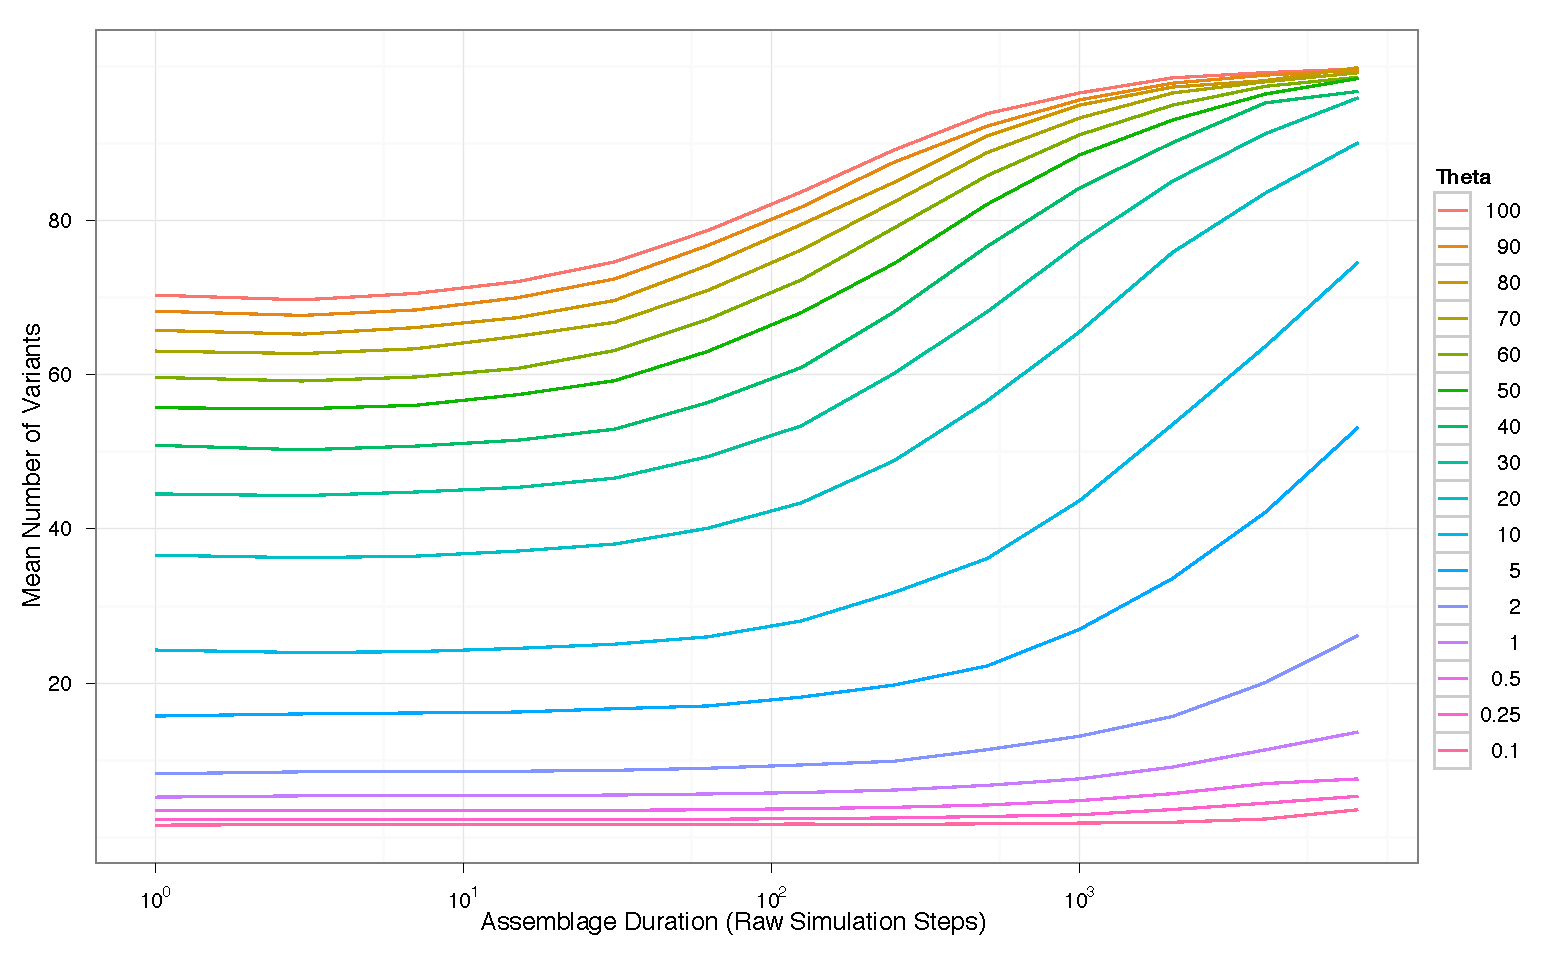
\includegraphics[angle=90, scale=0.75]{graphics/timeaveraging/unscaled_kn_by_duration_stacked.pdf}
	\caption{Mean value of $K_n$ for \timeavd samples, plotted against assemblage duration in simulation steps, for each level of $\theta$ in the study.  Note that the ``onset'' of \timeav effects (as measured by increased $K_n$), is quite gradual at low $\theta$, while high innovation rates display increased richness with very minor amounts of \timeav.}
	\label{fig:unscaled_kn}
\end{figure*}

\subsection{Neutrality Testing}
\label{sec:slatkin-ta-effects}

The Slatkin Exact test for neutrality, discussed in Section \ref{ta:sec:neutrality-test}, determines the ``tail'' probability for a sample of size $n$, with observed number of traits $k$, to be derived from the Ewens Sampling Formula (Equation \ref{eq:conditional-esd}).  The test employed in this study is Slatkin's Monte Carlo version, which allows the use of larger sample sizes, using random selection to create unlabeled configurations from the ESD to compare against the observed values.  The resulting tail probability is converted into a standard hypothesis test by selecting an $\alpha$ value.  For purposes of this study, I considered the upper and lower 5\% of tail probabilities to indicate that a sample was probably not derived from a neutral transmission model, leading to $\alpha = 0.10$.  

Given this $\alpha$ level, we should expect roughly 5\% of the samples taken from a pure neutral copying process to fall into each of the the upper and lower tail regions, and thus for a Slatkin Exact test to reject the null hypothesis of neutrality.  Roughly 90\% of the samples we take from the neutral WF-IA process should fall between $0.05 < p < 0.95$ and thus lead to acceptance of the null hypothesis.  This experimental setup also implies the limited utility of performing a single neutrality test on a single sample of class counts or frequencies, as has been archaeological practice by necessity.  A single Slatkin exact test with $\mathbb{P}_e$ value of, say, 0.96, would constitute some, but relatively weak, evidence of non-neutrality.  Better practice would be taking many samples from a large assemblage or multiple collections and calculating independent Slatkin tests for each sample, and examining their distribution.  

If \timeav has no effect on the validity of the Slatkin Exact test employed against temporally aggregated samples, we would expect the fraction of samples in the two tails (upper and lower 5\% in this case) to equal 10\%.  Anything over 10\% would constitute evidence of extra Type I errors, since we know the samples to have been generated by a process meeting the definition of the null hypothesis.  Therefore, after post-processing the simulation output to produce Slatkin tests as described in Section \ref{ta:sec:methods}, I tabulated the fraction of Slatkin Exact tail probabilities that exceeded the expected 10\% tail population.  These are, in other words, ``excess'' failures of the Slatkin Exact test, beyond those expected by the probability distribution itself.  For each $\theta$ level, and for each \timeav duration, the mean ``excess'' failure rate was computed, from the 1,113,134 raw Slatkin Exact test results generated in the simulation study.  

\begin{figure*}
%\centering
	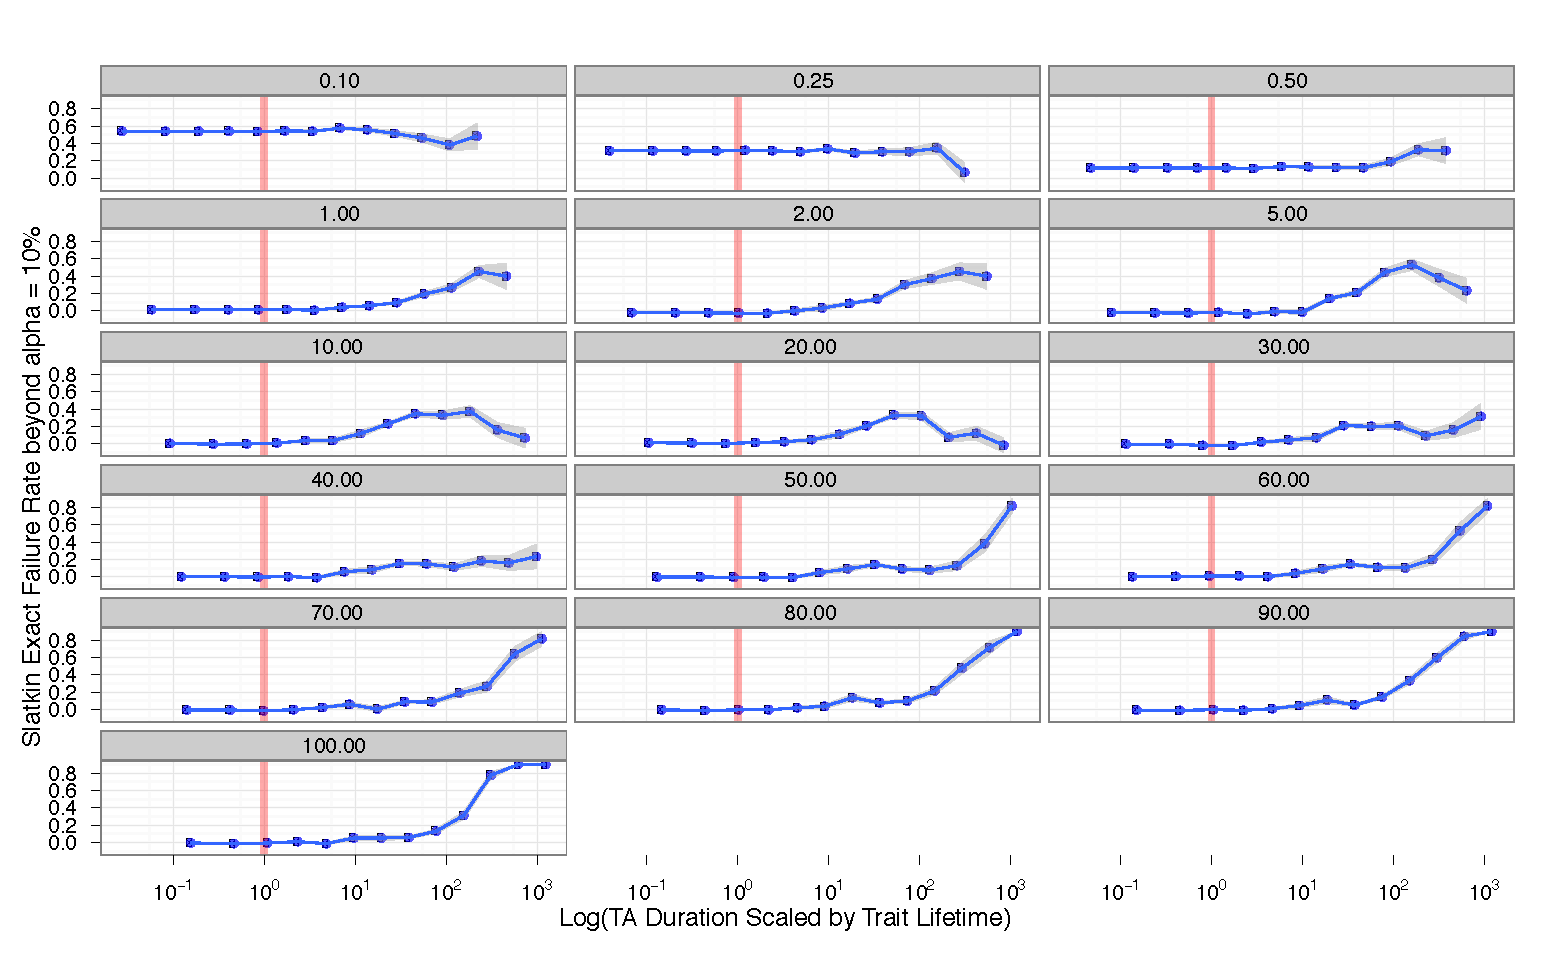
\includegraphics[angle=90, scale=0.75]{graphics/timeaveraging/slatkin-test-theta-0_1-100-100-5k-40k-failure-means-with-abline-labels.pdf}
	\caption{Slatkin Exact test failure rate (above the expected 10\% given two-tailed test with $\alpha = 0.10$, plotted against \timeav duration scaled by mean trait lifetime, for each level of $\theta$ in the simulation study. The red vertical line indicates the mean trait lifetime for that $\theta$ value, and the shaded region encompasses the standard error of the estimates for mean failure rates at each duration.}
	\label{fig:extra-slatkin-failures-by-scaled-duration}
\end{figure*}

Figure \ref{fig:extra-slatkin-failures-by-scaled-duration} depicts the relationship between the excess failure rate, and \timeav duration scaled by the mean trait lifetime (as previously described).  The mean trait lifetime is indicated by a vertical red bar in each graph.  Three major results are apparent.  First, at values of $\theta \geq 1.0$, the excess failure rate in non-time-averaged data is zero, as one would expect, and then begins to increase (albeit slowly) as the \timeav duration of samples exceeds the mean trait lifetime.  In some cases, such as $\theta = 5.0$, the Slatkin Exact test continues to be accurate given the chosen $\alpha$ value through samples which are aggregated for 10 times the mean trait lifetime.  But in all cases, with sufficient \timeav, the Slatkin Exact test begins to suffer from increased Type I error, reporting an ever increasing fraction of samples as not derived from a neutral transmission process.  The extreme situation is seen at very high rates of innovation, where nearly every test fails, at high levels of \timeav.  These failures are caused by saturation of a finite sample with singleton traits, causing the sample to display too much evenness in frequency to have been the result of sampling from the Ewens Sampling Formula.  But unrelated to this saturation effect, there is considerable failure in employing the Slatkin Exact test to detect neutrality.  For example, at $\theta = 5.0$, at 100 times the mean trait lifetime, approximately 70\% of all samples appear in the tail region of the distribution, compared to the expected 10\%.  Clearly, the Slatkin Exact test is not robust for long-duration assemblages.    

Second, at low $\theta$ values, the test results show excessive Type I error, even without \timeav.  There are several potential causes.  It is possible that the WF-IA process had not reached quasi-stationarity by 750 time steps, when sampling began.  This would mean that the effects of initial trait assignment might still be present and skewing the frequency distribution of traits.  Second, the Slatkin test is sensitive to the number of rare or singleton traits given the sample size, and in a small population (2000 individuals) with a low innovation rate (e.g., $\theta = 0.1$), counts of rare traits could be unstable.  This would not typically be the case in samples from large populations or entire species.  I do not consider the cause of this anomaly further in this paper, but it warrants further simulation study.   %Finally, at intermediate $\theta$ values (e.g., 10.0 - 30.0), the failure rate peaks at intermediate levels of \timeav, and then declines again).  This, too, is an unexplained effect warranting future research.

In general, with long-duration assemblages, archaeologists should be careful interpreting the results of neutrality tests adopted from population genetics.  The effect seen here can be summarized as:  with significant \timeav, trait frequencies generated by unbiased \ct can falsely appear to be non-neutral and thus driven by bias or selection (Type 1 error).  The longer the duration of an assemblage with respect to the mean trait lifetime, the larger the probability of a Type 1 error.  With sufficient duration, in fact, the probability of a Type 1 error becomes virtually certain, and the Slatkin Exact test loses any discriminatory power.  In summary, if one were to employ Slatkin's test to examine the hypothesis of neutrality in long-duration archaeological deposits, one would overwhelmingly come away with the impression that most \ct was biased, either towards conformity or a pro-novelty bias -- regardless of the underlying process occurring during prehistory.  

%It is worth noting that the effect appears to work in reverse when the data are known to be generated by a biased transmission process, such as conformist transmission.  Given the space constraints of a conference presentation, I leave the details of biased transmission models to another paper, but I performed a preliminary analysis of the conformist transmission model used by \citet{Mesoudi2009}.\footnote{Alex Mesoudi graciously provided the source code for simulations used in their paper, and I constructed a \tf module which replicated their exact algorithm for conformity.}  At even reasonably low levels of conformity (only a 10\% chance of a copying event being conformist rather than unbiased), Slatkin Exact tests upon unaveraged samples universally rejected the $H_o$ of neutrality -- virtually all samples concentrated themselves into the upper tail region.  At very high levels of \timeav, however, the null hypothesis began to be accepted, although at low frequency.  
%
%I conjecture that at low levels of conformist bias, and in relatively long duration assemblages, there can be equifinality between unbiased and conformist models, with respect to tests which fit trait counts to Equation \ref{eq:conditional-esd}.  This equifinality could be resolved, however, with a sufficient number of independent samples Slatkin Exact tests, since even a \timeavd unbiased process generates $\mathbb{P}(E)$ in both halves of the ESF distribution, whereas a pure conformist process under \timeav may generate $\mathbb{P}(E)$ values into the non-tail region of the ESF, but only from above, and not symmetrically around the center of mass of the ESF.  


%Clearly, we need to develop tests which can reliably distinguish neutral from biased transmission processes in the presence of significant \timeav.   Furthermore, when we compare results between assemblages, making an argument that some assemblages are more likely to be the result of (for example) conformist transmission, as opposed to unbiased transmission in other assemblages, the assemblage durations should either be approximately equal (with respect to the mean trait lifetime, which sets the timescale for such comparisons), or we need to consider the effect of the differential in durations when interpreting the test results.  

\subsection{Theta Estimation and Innovation Rates}
\label{ta:sec:theta-estimation-results}

There would be considerable value in estimating the population-level innovation rate ($\theta$) from sample data if it could be done accurately.  As discussed in Section \ref{ta:sec:theta-estimation-theory} above, such estimates are usually biased and have large variance.  In this section, I examine the effects of \timeav upon theta estimates generated from the samples taken to perform neutrality tests in the previous section.  For each of the 1.1 million samples of variants (distributed across actual theta values and assemblage durations), I calculated theta estimates given Watterson's approximation \citep{durrett2008}:

\begin{equation}
\label{eq:watterson-theta-est}
	\hat{\theta} \approx \frac{k_n}{log\;n}
\end{equation}

For each combination of actual theta and assemblage duration, theta estimates were averaged, to give a mean estimated theta value ($\mathbb{E}(\hat{\theta})$), and its standard deviation.  The results are shown in Table \ref{tab:estimated-theta-unaveraged}.   There are two regions of behavior apparent in the table, corresponding to drift- versus innovation-dominated dynamics.  At and below $\theta = 1.0$, estimated values are higher than the actual $\theta$ used to generate samples, and above 1.0, theta estimates begin to systematically lag below the actual theta value.  Overestimation at $\theta \leq 1.0$ matches the simulation results by \citet{ewens1974note}, although the authors did not simulate innovation rates above 2.0 (a large value in most genetic situations).  In addition to being biased, theta estimation appears to be even \emph{approximately} accurate only within a narrow range of values around $\theta = 1.0$.  

\begin{table}[ht]
\begin{tabular}{|c|c|c|}
  \hline
$\theta_0$ & $\mathbb{E}(\hat{\theta})$ & $\sigma(\hat{\theta})$ \\ 
  \hline
0.10 & 0.36 & 0.21 \\ 
  0.25 & 0.50 & 0.26 \\ 
  0.50 & 0.76 & 0.33 \\ 
  1.00 & 1.17 & 0.42 \\ 
  2.00 & 1.85 & 0.51 \\ 
  5.00 & 3.49 & 0.67 \\ 
  10.00 & 5.23 & 0.87 \\ 
  20.00 & 7.93 & 0.95 \\ 
  30.00 & 9.70 & 0.99 \\ 
  40.00 & 10.99 & 0.99 \\ 
  50.00 & 12.19 & 1.00 \\ 
  60.00 & 12.94 & 1.01 \\ 
  70.00 & 13.76 & 0.97 \\ 
  80.00 & 14.32 & 0.98 \\ 
  90.00 & 14.85 & 0.94 \\ 
  100.00 & 15.27 & 0.95 \\ 
   \hline
\end{tabular}
\caption{Mean Estimated Theta ($\mathbb{E}(\hat{\theta})$) from Samples (n=100) compared to actual values employed in simulation models ($\theta_0$), without any time-averaging.}
\label{tab:estimated-theta-unaveraged}
\end{table}

Figure \ref{fig:theta-estimates} examines estimates of theta by \timeav duration scaled by the mean trait lifetime, for each level of actual $\theta$ used in the simulation runs.  The pattern evident in synchronic or unaveraged samples carries over to \timeavd assemblages:  below $\theta \leq 1.0$, theta estimates are larger than the actual values, and increase in a non-linear fashion with assemblage duration.  Above 1.0 but below about 30.0, theta estimates begin below the actual value, cross the actual value, and continue to accumulate as assemblage duration increases.  Finally, at the very highest innovation rates, in a sample size 100, theta estimates are always drastic underestimates of the actual value, even with long assemblage duration increasing the accumulation of traits.  

\begin{figure*}
%\centering
	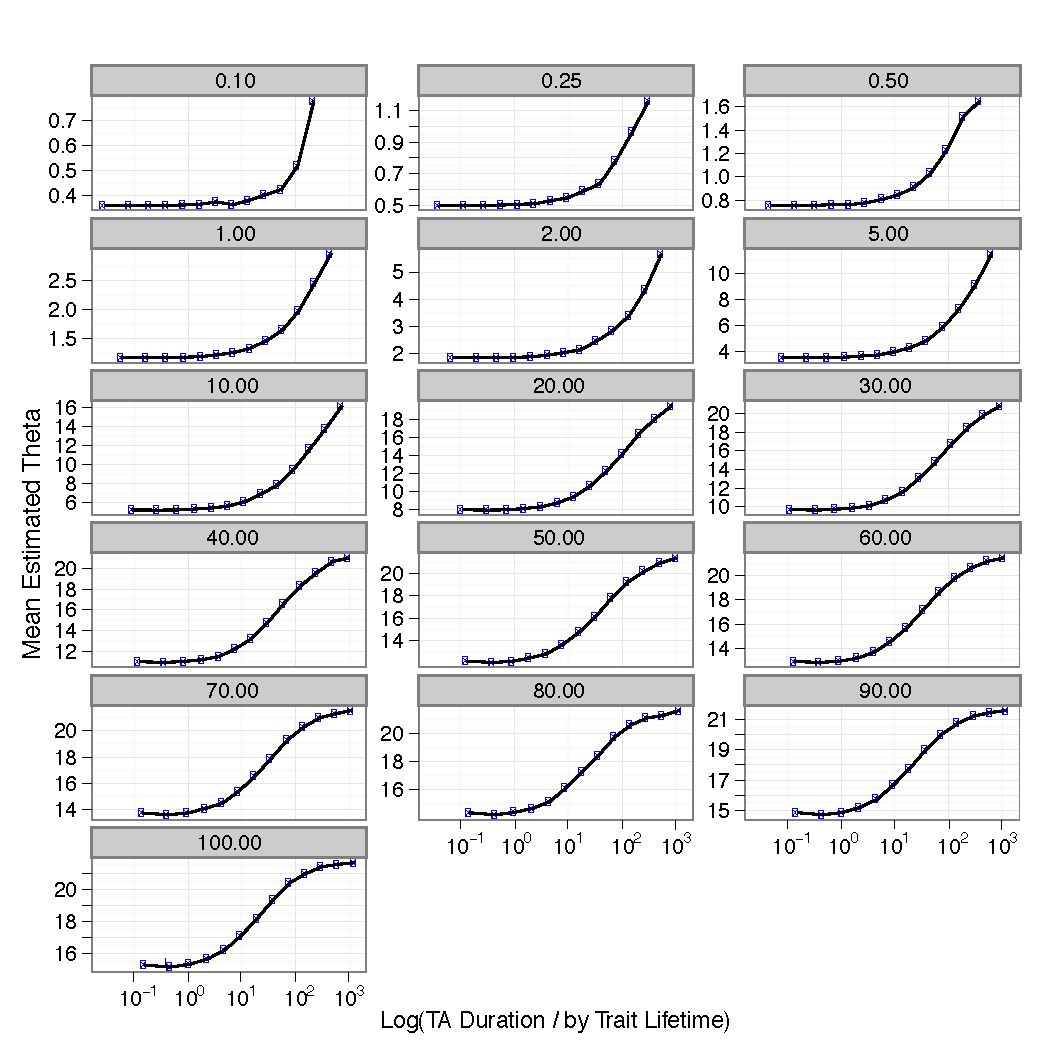
\includegraphics[scale=0.85]{graphics/timeaveraging/theta-estimates-scaled-MTL-theta-01-100.pdf}
	\caption{Estimates of mean population innovation rate ($\mathbb{E}(\hat{\theta})$) from samples ($n = 100$) taken for neutrality tests, using the approximation by \citet{watterson1975number}.  Plotted against assemblage duration, for each level of actual innovation rate used in simulation runs. }
	\label{fig:theta-estimates}
\end{figure*}

The Slatkin Exact test software also provides an estimate of $\theta$, finding the maximum likelihood value of theta when $K_n$ is set in Equation \ref{eq:expected-kn} to equal the observed value (this is the $t_e$ statistic introduced to archaeological usage in \citealp{Neiman1995}).  Figure \ref{fig:theta-estimates-slatkin} depicts the Slatkin theta estimates by \timeav duration scaled by the mean trait lifetime, for each level of actual $\theta$ used in the simulation runs.  One interesting difference between Figure \ref{fig:theta-estimates} and the Slatkin theta estimates is that the latter are more accurate for actual $\theta \geq 1.0$ than the Watterson approximation, in unaveraged assemblages.  Unfortunately, with increased assemblage duration, estimates explode to much larger values than those calculated by the Watterson approximation (i.e., $\theta \approx 1500$ for true $\theta = 30$ at maximum assemblage duration of 1000 times the mean trait lifetime, compared to the \emph{underestimate} of approximately 22 in Figure \ref{fig:theta-estimates}). 

\begin{figure*}
%\centering
	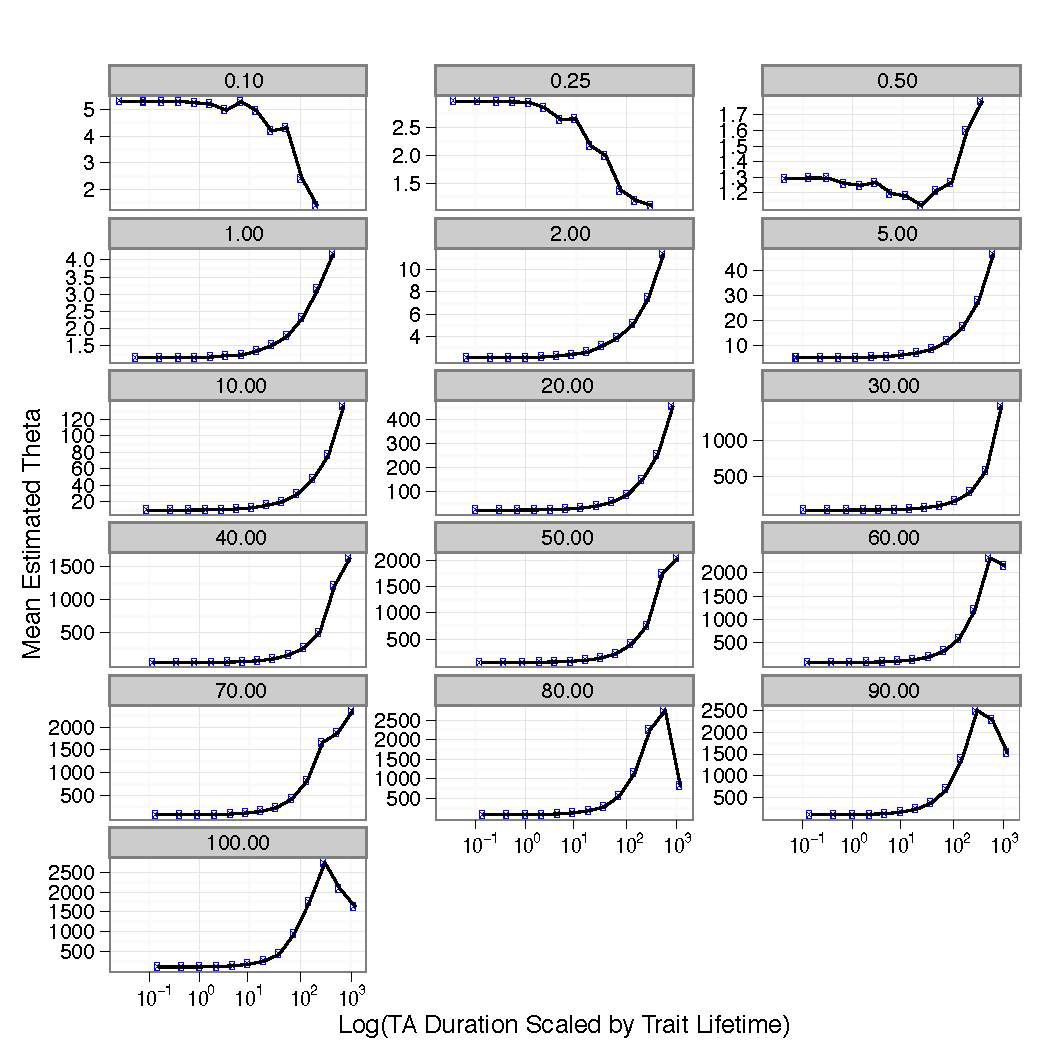
\includegraphics[scale=0.85]{graphics/timeaveraging/theta-estimates-scaled-Slatkin-theta-01-100.pdf}
	\caption{Estimates of mean population innovation rate ($\mathbb{E}(\hat{\theta})$) from samples ($n = 100$) taken for neutrality tests, using results from Montgomery Slatkin's neutrality test software.  Plotted against assemblage duration, for each level of actual innovation rate used in simulation runs. }
	\label{fig:theta-estimates-slatkin}
\end{figure*}

In short, estimation of population-level innovation rates from samples of artifacts using either estimation method are inaccurate, and the \timeav effect of accretional deposition renders such estimates even more inaccurate.  Clearly, such values cannot be used as actual indications of innovation rate or to ``work backward'' towards past population sizes.  And without fairly precise control over assemblage duration, the use of $t_e$ as a relative diversity measure between assemblages (in the manner common to archaeological applications) is highly suspect.  In the next section, I turn to $t_f$, the other common diversity measure in archaeological studies, which does not require an estimate of $\theta$, employing instead the variant frequencies directly.    

\subsection{Diversity Measures}\label{ta:sec:results-diversity}

Much of the current effort in distinguishing biased and unbiased transmission models rely upon trait evenness and the shape of frequency distributions, given Alex Bentley's application of power-law distributions to both ancient and contemporary data sets \citep{Bentley2003,bentley2004random,Bentley2007,bentley2007fashion, bentley2009physical,8913,8914}.  One of the ways that unbiased and ``conformist'' models of \ct differ is in the expected amount of variation.  Compared to unbiased transmission, conformism of even a mild degree tends to strongly concentrate adoption onto a very small number of traits \citep{Mesoudi2009}.\footnote{This is especially the case when conformist transmission is implemented in simulations as a ``global'' rule where only the most common trait is copied during ``conformist'' copying events, rather than weighting all traits by their relative popularity.  Very little work has been done to compare the results from different methods of simulating biased transmission models.  This is a topic which would benefit greatly from additional research.}  It is difficult, however, to interpret the absolute number of traits ($K_n$) without knowledge of the population size, so \citet{8977} employed diversity measures instead in his classic examination of conformist transmission in Southwest pottery.  

\begin{figure*}
%\centering
	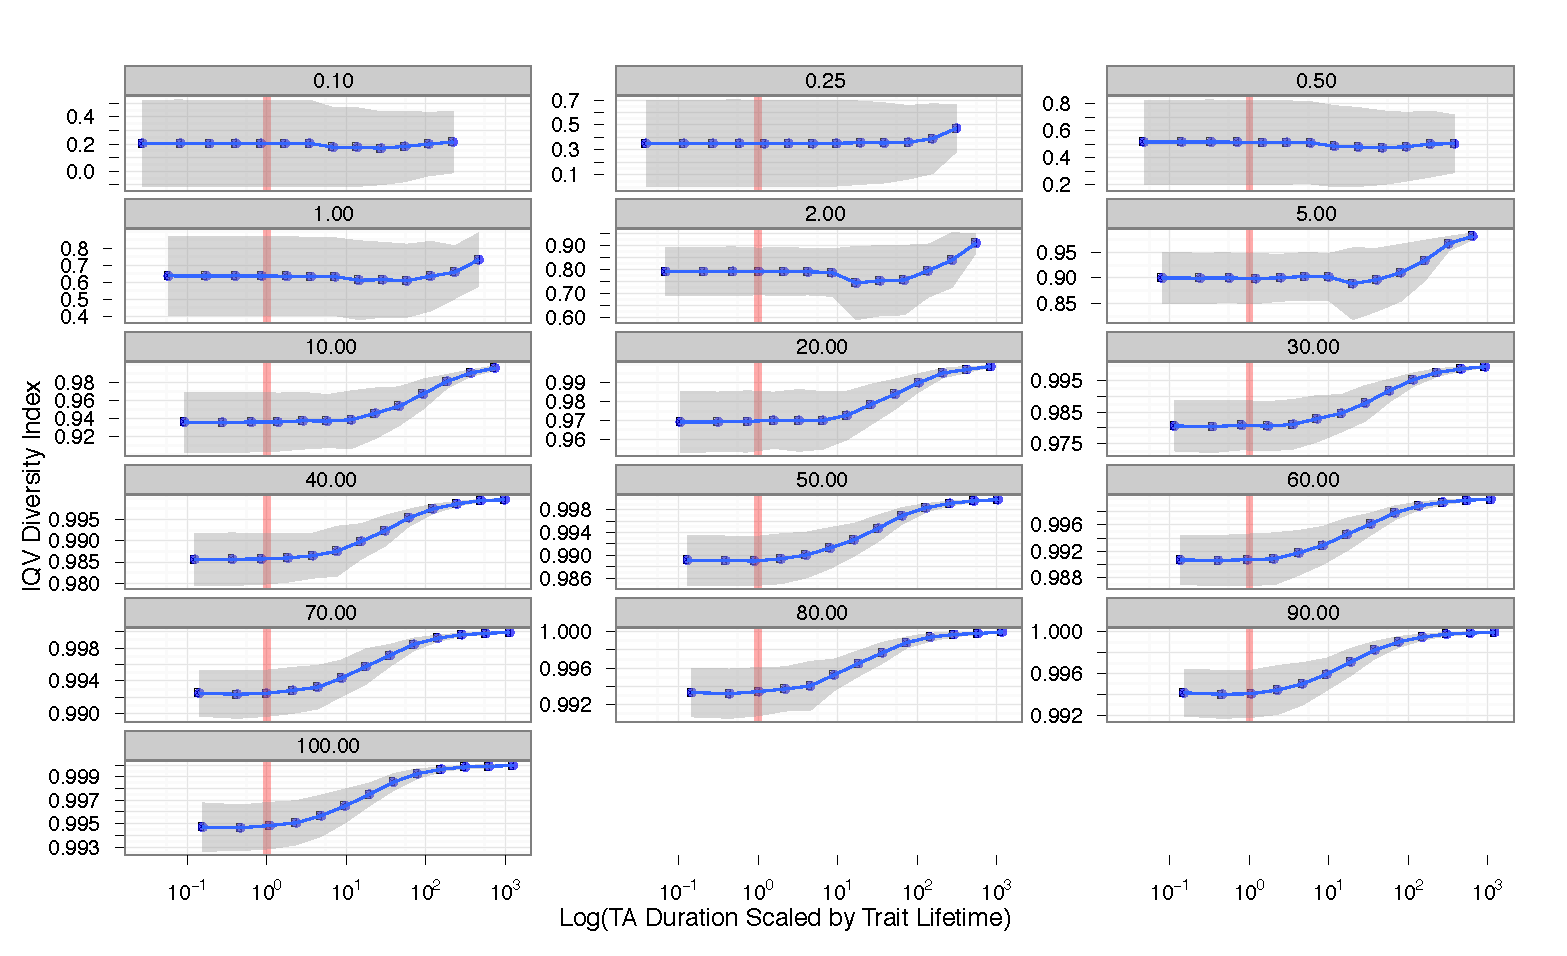
\includegraphics[angle=90, scale=0.75]{graphics/timeaveraging/wf-0_1-100-100-iqv-index-abline-labels.pdf}
	\caption{IQV diversity index, derived from samples of size 100, plotted against \timeav duration scaled by mean trait lifetime, for each level of $\theta$ in the simulation study. The red vertical line indicates the mean trait lifetime for that $\theta$ value.}
	\label{fig:iqv-est-by-scaled-duration}
\end{figure*}  

The most commonly used measure in the archaeological literature on \ct is $t_f$ (Equation \ref{eq:tf-formula}), since it is related to Wright's original measures of heterozygosity and thus associated directly with the historical development of the Wright-Fisher model.  But it is useful to normalize the results of $t_f$ between 0 and 1 so that we can compare different levels of theta and assemblage durations easily, in the same way that statisticians occasionally employ coefficients of variation or normalize covariances into correlation coefficients.  Equation \ref{eq:iqv-formula} does exactly this, and is called the ``index of qualitative variation'' (IQV) \citep{wilcox1973indices}.

Figure \ref{fig:iqv-est-by-scaled-duration} displays the relationship between the IQV for samples of size 100, and \timeav duration scaled by mean trait lifetime, as before.  IQV values range from 0.0, if only a single trait occurred within a sample (which happens in simulations with very low innovation rates), through 1.0, which indicates that traits are perfectly evenly distributed within a sample.  Even at the highest innovation rate studied, values of 1.0 were not seen in \emph{unaveraged} samples from the simulation runs.  It is apparent that \timeav can yield greater evenness among trait frequencies, although the plateau in IQV values  seen at high $\theta$ and high assemblage duration is a function of the saturation of $K_n$ in a finite sample seen above.  At very low innovation rates ($\theta \ll 1.0$), \timeav in contrast seems to have little effect on the dispersion of trait frequencies, with one or a very few traits always dominating a sample.



In between, when innovation rates are sufficient to guarantee at least one innovation on average per model generation ($\theta = 1.0$) but fewer than 10, there is non-monotonic behavior apparent in the IQV index.  For example, at $\theta = 2.0$, \timeav has no effect on IQV until duration is 10 times the mean trait lifetime (\mtl), at which point assemblages begin to appear \emph{less even} in frequency distribution, until about 100 times the mean trait lifetime, when evenness begins to steadily increase.   This effect is interesting, since it suggests that we cannot easily compare diversity indices between assemblages unless we control for duration or have independent evidence concerning innovation rates.   
 

\section{Discussion and Conclusions}
\label{ta:sec:conclusions}

When we examine the effects of \timeav on the sample properties of unbiased transmission, using the mean lifetime of traits as our fundamental time scale, several lessons for practical applications emerge.  First, it appears that assemblages with very small amounts of temporal aggregation display little of the distributional alterations that characterize long-duration assemblages.  Statistical tests of neutrality and diversity measures, and thus arguments based on them, can probably be used with care.   Second, estimates of population-level innovation rate derived from Ewens's sampling formula are biased (and therefore inaccurate), and become seriously inaccurate with increased assemblage duration.  Archaeologists should strongly reconsider using $t_e$ or other theta estimates even in relative comparisons, and should definitely not consider such estimates to reflect the innovation rate or population size present in the prehistoric population.  Third, for assemblages that have a duration longer than the mean trait lifetime, it is important to measure and control for the relative duration of assemblages when comparing statistical results across samples.  Without doing so, we cannot interpret relative differences of diversity indices or trait richness values as indicative of different modes of transmission.  

One caveat to the above is that such effects refer specifically to \emph{assemblage} level data, composed of many artifacts deposited over time.  Artifact-scale analysis, where the attributes under analysis come together in a short period of time, and where single artifacts comprise the counting unit for transmission studies, will not necessarily suffer the quantitative effects described here, or would suffer no measurable \timeav effects if the assemblage durations were short compared to the lifetime of traits.  A good example of this is Jonathan Scholnick's chapter in the present issue, expanding on his previous research into \ct in Colonial America through gravestones \citep{premo2011spatial,scholnick2010apprenticeship}, where his samples cover 10 year periods based on the death dates carved on each stone.  

Furthermore, while the mean lifetime of transmitted information plays a central role in establishing a ``natural'' time scale over which \timeav affects  unbiased transmission, this time scale is not an archaeological one.  This discrepancy in time scales arises because the abstract ``traits'' of our models are not equivalent to the classification units employed by archaeologists.  This is not a trivial difference, and is one that is rarely even discussed in archaeological applications of \ct models.  Instead, we frequently act as if  ``traits equal types,'' despite occasional acknowledgement of the difference. 

But we have no direct empirical access to the information prehistoric populations were learning, teaching, and imitating.  We will never find ``units of transmission'' in any empirical sense for archaeological applications of \ct models, and we have no warrant to equate our models of prehistoric information flow with the classes we use to observe it today.  Long ago, \citet{8874} recognized that when anthropologists study the ideas held within a social group under study, what is actually being studied are the ideas we \emph{construct} about the ideas individuals in other cultures may have had.  \citet{Dunnell1971} systematized this distinction, pointing out that we always operate with analytic classes whose construction is done by archaeologists, for archaeological purposes.  These classes serve as a ``filter'' by which we detect patterns in artifact assemblages, which reflect patterns in the information which flowed within past populations.  There is no ``natural'' set of classes to employ in studying \ct, but we often forget to incorporate this fact into our analyses.  Linking the time scale over which variation entered and left a prehistoric population, and the time scale over which archaeological classes appear and then exit the archaeological record will involve further research on the relationship between transmission dynamics and complex, multi-dimensional archaeological classes.  Such research is essential to connect the abstract quantities described by theoretical models, to observable aspects of the archaeological record.  

These results paint a fairly gloomy picture of almost all of the standard variables archaeologists have used since Neiman's \citeyearpar{Neiman1995} pioneering work.  One wonders why empirical studies using diversity measures, innovation rate estimates, or neutrality tests appear to ``work'' and give sensible results?  One possibility, of course, is that some studies don't yield the expected results.  We see this, possibly, in a fascinating analysis by \citet{steele2010ceramic}.  The authors employed ceramic classes that appeared to be non-neutral and subject to selection or biased transmission.  Yet Slatkin exact tests were unable to rule out the null hypothesis of neutrality.  I do not present an analysis of conformist transmission under \timeav in this article, but using \tf I see evidence that temporal aggregation has the opposite effect on Slatkin exact tests in populations with weak conformist biases:  neutrality tests suffer increased Type II error, making it more likely that we will accept a null hypothesis of neutrality when the opposite is the case.  

Another possibility is that certain variables may retain their distributional character, but have their values inflated by temporal aggregation.  In such situations, there would be no reason to reject the neutral model, but inferences about the values of parameters would be inaccurate.  Even if investigators did not rely upon the absolute value of parameters, frequently such inferences (e.g., diversity values) are employed as relative comparisons between assemblages.   I suspect that this has occurred in a number of published studies, but few \ct applications include detailed information concerning assemblage duration, so it is difficult to redo the researcher's original hypothesis tests with temporal controls, without going back to original field information or reports.  Clearly, both possibilities may also occur in some situations.  

As archaeological usage of \ct theory becomes more frequent and we move from proof-of-concept studies to demanding interpretive accuracy from our models, methodological research is essential to ensure that our applications are empirically and dynamically sufficient.  The present study focused on a necessary first step in such method development, developing an understanding of the effect of \timeav in accretional assemblages upon the observable variables in neutral \ct models.  The results demonstrate that frequently employed statistics, such as $t_e$, are highly inaccurate and biased when measured in \timeavd assemblages, and that neutrality tests are subject to enough additional Type I or Type II error that the results can be systematically misleading.  Clearly, in order to apply \ct models to diachronic data derived from \timeavd assemblages, we need to develop observational tools and methods suited specifically to the archaeological record, instead of simply borrowing statistical methods and models from theoretical population biology.  



\section{Acknowledgements}
This paper was originally presented in a symposium titled \emph{``Recent Developments in Cultural Transmission Theory and its Applications''} at the 2012 Annual Meeting of the Society for American Archaeology, Memphis, TN.  The author wishes to thank Kristen Safi, the organizer, for the opportunity to participate, and Carl P. Lipo, Fraser Neiman, James Feathers, Jonathan Scholnick, and Michael J. O'Brien for comments on drafts of this paper. 






    
    \chapter{Can We Identify Transmission Bias in the Archaeological Record:  An Investigation Using Boosted Classifier Models}
    \label{chap:ctmixtures-paper}
    \begin{description}[leftmargin=-1\labelwidth]
\item[\textsc{Abstract}] \lipsum[1] 

\item[\textsc{Source}]  Posted to Arxiv.org (\url{https://arxiv.org/abs/TBD}), in July 2019.  
\end{description}


\section{Introduction}\label{introduction}

A major use of cultural transmission models in archaeology is inference
regarding the mode of transmission operative within past populations.
Identifying cognitive biases is central, for example, to several
hypotheses for the origin of cumulative cultural transmission and
complex culture \cite{BR1985, CF1981, Henrich:1998ek, Wakano:2007gq}.
In more recent archaeological contexts, the identification of
frequency-biased social learning has been used to support
inferences concerning sociopolitical structure 
in past societies \cite{kohler2004}.  Simulation and mathematical
studies have yielded many insights into the empirical patterns we can expect from different transmission models
\cite{Bentley2003, bentley2007regular, bentley2004random, Evans:2011vm, Mesoudi2009},
although much of this knowledge is derived from very simplified
population models.  In particular, theoretical analyses of transmission models  have ignored until recently the effect of data collection methods and coarse-grained observations on the patterns we should expect in archaeological data.  As a result, we simply do not know whether the mode of transmission can be reliably inferred from samples of the archaeological record, if it is possible at some time scales but not others, or how we might tailor data collection strategies to maximize the accuracy of such inferences.


We do know that the coarse graining of observable variables that occurs given time averaging reduces our ability to distinguish between
unbiased and biased transmission models
\cite{Madsen2012TA, Porcic2014Exploring-the-E, Premo:2014jv}, that non stationary
population sizes reduce our ability to infer transmission modes \cite{Rorabaugh:2014fl}, and that
diachronic statistics and non equilibrium models are better than
synchronic measures and equilibrium models 
\cite{kandler2013non, wilderkandler2015}.  The effect of these factors is such that when deposits are highly time averaged, equifinality occurs, with different models yielding the same empirical distributions despite describing different underlying processes \cite{von1949problems}. Equifinality between
theoretical models is a serious concern whenever we study complex
systems, and has been discussed in geomorphology, hydrology,
climatology, and within archaeology itself
\cite{Aronica:1998dm, Beven:2006js, Bonham:2009bi, Cicchetti:1996gp, 
Culling:1987kx, Marean:1992hg, Rogers:2000bq, Savenije:2001fe}.
If models which represent different modes of cultural transmission
cannot be distinguished when we include aggregation, heterogeneity, or sampling in our models,
then there may be questions concerning past cultural transmission that
we cannot answer.  As a result, there may be classes of models which are useful for contemporary or historical 
research, but not for the coarse grained scales of observation that archaeologists often confront.

Existing theoretical studies have almost exclusively focused upon distinguishing
models based on the ability of a single statistic or variable to
distinguish the distribution of outcomes from different social learning
modes. Scores from the power law exponent
in a log-log plot of trait frequencies have received the most attention along with more recent application of neutrality tests \cite{Bentley2003, bentley2004random, Mesoudi2009, slatkin1994exact, slatkin1996correction}.   
More recently, Kandler's work has demonstrated that diachronic measures such
as trait survival time, or the length of time the most common trait
stays ranked the most common, can be robust predictors of different
classes of transmission models
\cite{kandler2013non, wilderkandler2015}. 
But there is little reason to suspect that single statistics will be adequate in most cases to cleanly separate and identify different transmission models, given the strong convergence in distribution that characterize diffusion processes.  Instead, we should expect that statistical models employing multiple predictors would be the best discrimination tools, if any exist for a set of transmission models.  In this paper, I employ
a robust machine learning classifier algorithm and multiple ways of measuring
trait richness, diversity, and survival times to test whether
equifinalities exist between various combinations of unbiased and biased
transmission rules when measurements come from realistic data collection
scenarios.\footnote{Throughout this paper, I used ``classification'' in the statistical and machine-learning sense of a statistical model whose dependent variable is a binary or discrete value, such that the model predicts which value a data point takes from a labeled set.  Archaeologists will be used to using the term in the sense of systematics and taxonomy, which is not the intent here.}

The results indicate that while neutral and biased transmission models
can be distinguished very accurately given measurements from entire
populations taken when no temporal aggregation occurs, the introduction of
sampling and the interaction between sampling and time averaging
 markedly degrades our ability to distinguish these transmission
rules. Furthermore, the degradation is not symmetric. With sampled, time
averaged data, we are extremely likely to conclude that samples
represent biased transmission, even when this is not the case. Other
mixtures of conformist and anti-conformist transmission rules are even
less distinguishable given time averaging and limited samples.  As a result, I conclude that it may be difficult or impossible to infer the details of cognitively biased transmission rules from frequency data alone, when we lack data from an entire population and when only coarse grained, aggregated data are available.

\section{Analysis}\label{analysis}

\subsection{Reducible and Irreducible Equifinality Among Transmission
Models}\label{measuring-equifinality-among-transmission-models}

Equifinality among cultural transmission models can arise from several sources. First, equifinality may occur because of our measurement and analysis
procedures. There is growing evidence, for example, that assemblage
duration affects our ability to distinguish biased from neutral
transmission across a variety of statistical predictors
\cite{Madsen2012TA, Porcic2014Exploring-the-E, Premo:2014jv}. Equifinality among transmission models is thus possibly reducible by collecting finer-grained samples during fieldwork, if deposits are well stratified.  However, in situations where the depositional environment actively creates temporal aggregation (e.g., in the plowzone, or in deflated aeolian contexts), there may be little that an investigator can do to improve the temporal resolution of data collection.  And when we employ published data sets, obviously we cannot easily subdivide the data into assemblages finer than the original investigation supported.  When studying living populations, of course, equifinalities may be addressed by converting a purely observational study to a controlled experiment in some cases \cite{kempe2014experimental, mesoudi2014experimental, schillinger2014copying},
but of course this is not an option in archaeological contexts.

Second, equifinality is partially determined by the predictors or variables we use in trying to separate the behavior of models.  Fig. \ref{fig1} shows an artificial example with two distributions, measured on two variables.  The marginal distribution of each variable demonstrates how models might be distinguishable given one variable (Y axis) but not another (X axis).  In the published literature on transmission modes, single variables are usually examined, but we gain huge power by considering statistical models with multiple variables.  


\begin{figure}
	\caption{Simple example of the effect of variable choice in distinguishing models.  The variable on the X axis displays quite a bit of overlap between models, while the variable on the Y axis distinguishes the models with fairly high accuracy.}
	\label{fig1}
\end{figure}

Not all equifinalities may be reducible.  The statistical distributions generated by diffusion processes can be highly convergent among related models, and almost all cultural transmission models are, at base, diffusion processes. This type of equifinality is \textbf{irreducible}, and is not solved by changing how we perform the analysis or by changing data collection. Irreducibly equifinal
models form an \textbf{equivalence class} of models that we cannot
distinguish given our data. Instead, all we can say is that our data
could have been generated by any of the models in the equivalence class.  
If the equivalence classes of equifinal models are coarse enough (at worst, if they 
form a single group), then we cannot meet our original inferential goals at all. 

In some cases, irreducible equifinalities can become reducible given advances in measurement technologies that open up new sets of predictor variables.  After his seminal works of the 1970's on drift and the infinite-alleles neutral model, Warren Ewens stopped working on neutrality tests because tests using allele count data lack statistical power.  Ewens moved to studying the population genetics of human diseases instead \cite{plutinski2004}, recognizing that further progress would require sequence data unavailable at the time.  This judgment proved accurate:  a new suite of neutrality tests did arise starting the late 1980's and 1990's when sequence data became widely available \cite{fu1993statistical,tajima1989statistical}.     


\subsection{Equifinality As Classification Error}
\label{sec:equifinality-classification-error}

Since our evolutionary models of cultural transmission are stochastic, and generate a variety of outcomes for the same parameter values, I take a statistical approach to examining equifinality of transmission models in archaeological data.  Transmission modes are separable and thus identifiable in archaeological data if the distribution of model outcomes are non-overlapping, when measured in a space created by a set of predictor variables.  With stochastic models like the ones currently used by archaeologists, the most efficient method of studying the outcome distribution is to simulate values from the model, and examine our ability to correctly predict which model generated each data point, given a function of the predictor variables.  

This general approach can be visualized as in Fig.
\ref{fig2}. Here, three pairs of probability models
are represented by 500 measurements each of two continuous predictors variables (e.g., a diversity index).
In the left panel, the pair of models do not overlap in their outcomes.
Given a data point, we can assign it to Model 1 or Model 2 with
virtually no error, and thus we would consider models 1 and 2 to be
distinct and not equifinal at all. The situation in the middle and right
panels of Figure \ref{fig1} is different. There is
some overlap in the middle panel, and very strong overlap in the right
panel. In the right hand panel, in fact, there is enough overlap that on
average, our ability to assign a randomly chosen data point to the
correct model is no better than chance. Intuitively, we would say that
there is some equifinality in the middle panel, and that the two models
were strongly equifinal in the right hand panel.

\begin{figure}[h]
\caption{Simple example of model outcomes with different degrees of distinguishability: (A) simulated data point from two fully separate models, (B) two models with a limited overlap region, (C) and two models whose outcomes are highly overlapping.}
\label{fig2}
\end{figure}


We can formalize the analysis of overlap between models as a problem of
``classification'' or ``pattern recognition'' in the sense of
statistical or machine learning \cite{hastie2009elements}. Given a set
of models \(\mathcal{M}_1 \ldots \mathcal{M}_n\), we can measure
equifinality as the minimum possible error achievable in correctly
assigning simulated data points to the models which generated them,
given measurement of a set of predictor variables. In general, the
classification problem asks which model has the highest probability for
a given data point, given the conditional density of the data and
models. This sounds exactly like Bayes' theorem, and in fact we can
write the classification problem as follows, where
\(Y \in 1, \ldots, K\) refers to each of \(k\) models, and
\(X_1, \ldots, X_p\) refer to \(p\) different predictor variables.

\begin{equation}
\mathbb{P}(Y | X_1, \ldots, X_p) = \frac{\mathbb{P}(Y_i) \mathbb{P}(X_1, \ldots, X_p | Y)}{\mathbb{P}(X_1, \ldots, X_p)}
\label{eq:bayes-rule-classification}
\end{equation}

\(\mathbb{P}(Y)\) plays the role of the prior distribution, and is the
prevalence of each model in the population. This is a constant in
situations where we are simulating values from each model to test for
equifinality. The data points in a classification problem are given, and
thus the denominator is a constant. The most probable class for a given
data point is just the mode of the likelihood function, which is given
by:

\begin{equation}
Y_{pred} = \argmax_y \mathbb{P}(X_1, \ldots, X_p | Y)
\label{eq:map-class-bayes}
\end{equation}

This is the \emph{Bayes classifier} for a controlled simulation
experiment, and its error rate in separating data points by model is
called the \emph{Bayes error}. This is the lowest possible error in
separating the models given the data
\cite{devijver1982pattern, fukunaga1990introduction, hastie2009elements}.
The Bayes error is zero when we can correctly identify each data point
as to its model of origin (as in the left panel of Fig. \ref{fig2}, and rises as two models overlap in the
measurement space. With sufficient overlap, the Bayes error could
approach 0.5, which represents a prediction rule which is no better than
chance.\footnote{Predictors can achieve even worse error levels, performing more poorly than coin-flipping, but in the current study we will not encounter such rates.}

Unfortunately, we can almost never directly calculate the Bayes error
rate for a prediction or classification rule, because we rarely have an
expression for the likelihood function of our transmission models in the
spaced formed by the predictor variables. Bayes error can be directly calculated, in fact, only for
a small number of cases, such as Gaussian distributions with a shared
covariance
matrix.\footnote{There is a large literature, especially in pattern recognition and language classification, on approximating upper bounds for the Bayes error of a classifier, because it is highly useful to know when you cannot improve a recognition system or classifier any further \cite{Antos:1999dn, Dobbin:2009du, McLachlan:1975eo}.  Most such upper bounds are based upon parametric models, and use estimates of a distance metric between the classes being distinguished (typically, the Mahalanobis or Bhattacharyya distance) \cite{devijver1982pattern}.  Such bounds are difficult to justify in situations where we have complex social learning models, whose probability density functions in the space of measured variables are typically unknown and are unlikely to be Gaussian.  Non parametric bounds are possible, using nearest-neighbor methods \cite{Loizou:1987bi}, but in most cases the values obtained are not very tight and the performance of boosting and bagged classifiers easily surpasses such methods.}
Despite the fact that we can rarely calculate the Bayes error rate, it
is useful as an operational definition for equifinality, since it
measures our uncertainty about model choice given a set of measurable
variables. In practice, we approximate the Bayes error by employing
algorithms which are known to have near-optimal performance in
classification problems. In particular, boosting, bagging, and ensemble
approaches that combine many classifier rules are attractive since each
achieves some of the best generalization error in prediction tests
\cite{hastie2009elements}, and thus come closest to estimating the
Bayes rate \cite{tumer2003bayes}.  


\subsection{Study Design}\label{model-comparisons}

In order to assess whether transmission bias is identifiable from archaeological samples, this study simulates conformist, anticonformist, and unbiased cultural transmission over a range of innovation rates, recording the outcome of transmission events in the form of counts for individual traits, and for cross-tabulated ``classes'' of traits which simulate multi-dimensional archaeological types of the kind typically used by archaeologists.  These samples of trait and class counts are then subjected to sampling and temporal aggregation, to simulate the kind of assemblage-level often confronted in archaeological samples.  For both the raw trait/class counts, and the sampled and time averaged counts, I use a classifier approach with multiple predictor variables to assess the identifiability of transmission bias.    

The general process followed throughout the study is:

\begin{itemize}
\itemsep1pt\parskip0pt\parsep0pt
\item
  Simulate a large number of samples from each cultural transmission
  model, at a fixed population size, but with an innovation rate drawn from a uniform distribution of possible values.  Record trait and class counts during sampling intervals and at the end of each simulation run.
\item
  Measure a set of archaeologically relevant variables (e.g., richness,
  diversity) on each stored sample.
\item
  Perform each variable measurement across different data collection
  regimes (e.g., duration of accumulation, sample size).
\item
  Train a predictive classifier model for each data collection regime,
  to predict the model of origin given the measured variables.
\item
  Assess the classifier error rate using additional samples simulated
  from each transmission model.
\end{itemize}





\subsection{Methods}\label{methods}

\subsubsection{Simulated Samples of Cultural Transmission
Models}\label{simulated-samples-of-cultural-transmission-models}

The outcomes of all four transmission models are derived by simulating the
dynamics of the model in an agent-based framework that allows each agent to be assigned a different transmission rule.  All simulations employ
the Moran dynamics, where one individual engages in a copying event at
each elemental step
\cite{moran1962statistical, moran1958random, aoki2011rates}.
Innovations are modeled using the ``infinite alleles'' approximation,
where every innovation is new to the population \cite{Ewens2004}.
Simulations were performed using the CTMixtures software package,
available as open source
software.\footnote{\url{https://github.com/mmadsen/ctmixtures}} The
parameters for all simulation runs are given in Table
\ref{tab:parameters}. Where there is a range given (e.g., innovation
rate), the parameter is treated as a prior distribution and each
simulation run is assigned a uniform random value from the range. This
ensures good coverage of the parameter space given 25,000 replicates for
each of the 4
models.\footnote{The use of a good prior distribution for parameter ranges also results in simulation data that are usable for later data fitting by approximate Bayesian inference \cite{Beaumont:2010ur, Crema:2014ef, Csillery:2010jd, marin2012}.}

\begin{table}[h]
\begin{tabular}{lc}
\hline
Parameter & Value or Interval \\ 
\hline
Innovation rate (in $\theta$ scaled units)  & $[0.1, 5.0]$   \\
Probability of conformism & $[0.05, 0.25]$ \\
Probability of anti-conformism & $[0.05, 0.25]$ \\
Sample fractions & 0.1 and 0.2 \\
Time averaging intervals (units of 100 individuals) & 10, 20, 50, 100 \\
Population size & 100 \\
Number of trait dimensions (loci) & 4 \\
Initial traits per dimension & 10 \\
\hline
\end{tabular}

\caption{Parameters for simulation runs across the four models studied.  Intervals are treated as prior distributions, and each simulation run is assigned values derived from a uniform random sample on the interval indicated.  Lists of values are all applied to every simulation run (e.g., there is both a 10\% and a 20\% sample from each simulation run.  Single values are applied to every simulation run, and represent a point prior.)}
\label{tab:parameters}
\end{table}

Simulated populations are 100 individuals in size, because most
archaeological studies of cultural transmission have focused upon
situations where population sizes are assumed to be small. 
Each simulated individual carries 4 different
traits at any time, which are treated as separate loci or dimensions.  Trait frequencies are tracked on a per-locus basis, and combinations of loci are tracked in order to simulate archaeological ``types'' or classes which include multiple dimensions of variation.

Regardless of transmission model, social learning involves no interaction effects between loci in this study. The
population is seeded with 10 randomly chosen traits at each locus as a
starting configuration. The evolution of each simulated population proceeds
for 4 million elemental steps, which is equivalent to about 40,000
copying events on average per individual. This value was chosen by
performing simulations at 1 million time step intervals and verifying
that the distribution of a key statistic (the number of traits per Loci)
had stabilized. This occurred in most cases between 2 and 3 million
steps, and in all cases between 3 and 4 million, so the last value
was chosen.\footnote{The analysis underpinning this decision is available in the Github repository at \url{https://github.com/mmadsen/experiment-ctmixtures/analysis/verification}.}
At the end of 4 million simulation steps, a suite of variables are
measured from each of the 25,000 replicates and stored for analysis.

\subsubsection{Variable Selection}\label{variable-selection}

Since most previous work on identifying transmission mode from archaeological data employ single diagnostic variables, and begin to display equifinality under realistic data collection conditions, it is reasonable to examine whether using multiple variables will yield more discriminatory power in the same contexts.  By representing the outcomes of transmission models in a higher dimensional space, it should be easier to find a decision boundary (``separating hyperplane'') that correctly predicts the model which generated each data point, if such a boundary exists.  

\begin{table}[ht]
\begin{tabular}{lll}
\hline
Variable                                    & Model Variable \\ 
\hline
Cross-Tabulated Class Richness  (Class)         &  num\_trait\_configurations      \\
Slatkin Exact (Class)           & configuration\_slatkin       \\
Shannon Entropy (Class)  &  config\_entropy \\
IQV Diversity (Class)  & config\_iqv \\
Neiman $T_f$ (Class) & config\_neiman\_tf \\
Slatkin Exact (Max for Locus)                    & slatkin\_locus\_max       \\
Slatkin Exact (Min for Locus)                     & slatkin\_locus\_min      \\
Slatkin Exact (Mean for Locus)                   & slatkin\_locus\_mean       \\
Shannon Entropy of Trait Frequencies (Min)      & entropy\_locus\_max       \\
Shannon Entropy of Trait Frequencies (Max)       & entropy\_locus\_min      \\
Shannon Entropy of Trait Frequencies (Mean)      & entropy\_locus\_mean      \\
IQV Diversity Index (Min)     & iqv\_locus\_max \\
IQV Diversity Index (Max)     & iqv\_locus\_min \\
IQV Diversity Index (Mean)    & iqv\_locus\_mean \\
Trait Richness (Min)   & richness\_locus\_max \\ 
Trait Richness (Max)   & richness\_locus\_min \\
Trait Richness (Mean)    & richness\_locus\_mean \\
Kandler-Shennan Trait Survival (Min)   & kandler\_locus\_max \\
Kandler-Shennan Trait Survival (Max)   & kandler\_locus\_min \\
Kandler-Shennan Trait Survival (Mean)   & kandler\_locus\_mean \\
Neiman $T_f$ (Min)   & neiman\_tf\_locus\_max \\
Neiman $T_f$ (Max)   & neiman\_tf\_locus\_min \\
Neiman $T_f$ (Mean)   & neiman\_tf\_locus\_mean \\
\hline

\end{tabular}

\caption{Variables measured from each transmission model simulation sample.  The parenthetical expression records whether the variable was calculated for cross-tabulations of all 4 loci (Class) or represent the order statistics from individual loci (Min/Mean/Max).  The right column records the variable name used within R statistical models, for examining the relative importance of each variable in classifying observations.}
\label{tab:variables}
\end{table}

The predictor variables chosen in this study focus upon measures of richness and
diversity, trait survival over time \cite{kandler2013non}, and the
Slatkin neutrality test \cite{slatkin1996correction, slatkin1994exact}.
Each has been employed in the archaeological literature on identifying
cultural transmission modes, or is a variant on such measures (e.g., IQV
is a normalized version of Shannon entropy), and crucially, all are measurable in standard archaeological contexts using type frequency data.  This additionally makes most of the variables applicable to the re-analysis of already published data, which is an important usage scenario in archaeological research.   

For the locus-centric variables, each statistic was applied to each
locus separately, and the mean, minimum, and maximum of the values
obtained for each locus were recorded. I collect order statistics
in addition to the mean value, since it is possible that minima and
maxima might be a better discriminator between models than averages. In
addition to the variables calculated upon each of the 4 loci, the traits
at each locus were combined into a cross-tabulation of "classes" which simulates the
process of archaeological classification. Each class represents a
different combination of traits from the 4 loci, and very roughly
simulates observing cultural variation through the lens of a standard
paradigmatic classification \cite{Dunnell1971}. The same variables are
then measured as a function of the class counts.\footnote{The sole exception is the Kandler-Shennan survival time, which is not measured here for the cross-tabulated classes.  Understanding the quantitative behavior of this measure for multidimensional classes of traits is an important open research question, however.} This allows us to
understand whether transmission models are better distinguished on a
per-locus (dimension) basis or by operating on more complex classes that
combine several traits together. The full list of measured variables is
given in Table \ref{tab:variables}.

As a final note on variable selection, in an exploratory analysis for this
project, I tried to include the power law exponent from a log-log
transformation of trait frequency, given the important work by Bentley
\cite{bentley2004random} and Mesoudi and Lycett
\cite{Mesoudi2009}. It is not clear, however, that previous uses
of this variable have been comparable to measurements we can make on
archaeological assemblages. As an example, Mesoudi and Lycett
\cite{Mesoudi2009} use the cumulative number of adoptions of each
trait over the entire time span of the simulation as the ``frequency''
used to calculate power law
exponents.\footnote{I confirmed this by inspection of the source code for their simulation model, which was provided by Alex Mesoudi.}
Given the measurement strategies described in Table
\ref{tab:measurement-strategies}, the number of traits present at any
given time is often small, and their prevalence in a small population
makes it difficult to fit a power law to the data. Despite its
importance in archaeological discussions of neutral versus biased
transmission, I have omitted power law exponents from the published
analysis, pending investigation of the proper method for calculating
them in situations with small \(N\) and small numbers of trait
categories.

\subsubsection{Data Collection Treatments}\label{data-collection-treatments}

At the end of each simulation run, after the model has reached a quasi-stable equilibrium (measured as stability in per-locus trait richness), a series of samples are taken from the evolving population.  These samples are taken in ways that correspond to various real-world data collection strategies.  First, a census of the entire population is taken.  This functions as a baseline for the ``most complete'' information we can use to identify transmission modes, and there are also conditions during observational studies or in laboratory experiments where census is possible.  In archaeological studies, anything approximating a census is usually impossible, although Jonathan Scholnick's study of New England gravestones and their makers may approximate this quality of data collection \cite{scholnick2012spatial}.  Second, the simulated population is sampled, at the 10\% and 20\% levels.  Sampled data is ubiquitous in archaeological research, and although the issues involved in mapping artifact samples to their meaning for the underlying population of social learners is complex and unresolved, it is useful to determine whether the overall sample fraction has a measurable effect upon model equifinality.  

Archaeological data are rarely synchronic or ``point in time'' samples of the results of human activity, and are typically aggregated over an appreciable duration of time through both data recovery conventions and formation processes \cite{grayson1998,lyman2003influence,Madsen2012TA,Porcic2014Exploring-the-E,Premo:2014jv}.  Thus, the sampled data employed in this study is also temporally aggregated over a number of time steps, and the aggregate trait counts and then used to determine the frequencies of cultural traits over the entire interval.  The population census has no temporal aggregation, and thus does represent a synchronic census.  

Time averaging is implemented according to the schematic in Fig. \ref{fig3}.  At the end of the simulation run, sampling begins at a time index calculated to allow time averaged samples to be taken twice, with a gap of 50 ``generations'' to allow the calculation of the Kandler-Shennan trait survival statistic (although unlike their original study, the values at the start and end times are inherently time averaged in this study, which would be the base in any real archaeological context) \cite{kandler2013non}.\footnote{The effect of time averaging on the start and end values used to calculate the Kandler-Shennan trait survival is not directly studied in this paper, but is a necessary component of using their method to study archaeological assemblages, I believe.}  

\begin{figure}[h]
	\caption{Schematic of how sampling is implemented in this study.  Time runs from the start of the simulation run at the top, to the end at the bottom.  The interval of time over which we calculate the Kandler-Shennan trait survival is given as a simulation parameter, and represents the gap in the middle of the diagram.  Before and after that gap are windows of successive duration, representing aggregation over 10, 25, 50, and 100 ``generations'' of the simulation.}
	\label{fig3}
\end{figure}


\begin{table}[ht]
    \begin{tabular}{lll}
        \hline
        Sampling Strategy & Time Averaging Duration \\ 
        \hline
        Population Census & 0 \\
        10\% Sample & 10 \\
        10\% Sample & 25  \\
        10\% Sample & 50 \\
        10\% Sample & 100 \\
        20\% Sample & 10  \\
        20\% Sample & 25 \\
        20\% Sample & 50 \\
        20\% Sample & 100 \\
        \hline
    \end{tabular}
    \caption{Data collection strategies, applied to every simulation run.  Time averaging duration is given in units of "generations," which are units of 100 time steps (given the population size).  100 generations thus represents 10,000 elemental time steps in the Moran simulation dynamics.}
    \label{tab:measurement-strategies}
\end{table}

The data collection strategies employed in this study are given in Table \ref{tab:measurement-strategies}.  Applied to all 23 variables, the study yielded approximately 900,000 samples from the four transmission models.\footnote{All data and analyses for this study are available as part of a Github repository, although large data files are kept on Amazon S3 for long-term storage.  See \url{https://github.com/mmadsen/experiment-ctmixtures} for details.  The published analysis described here is the ``equifinality-4'' data set.}  This raw data was then formed into the three pairwise comparisons shown in Table \ref{tab:comparisons} for equifinality analysis with a classifier model.

\subsubsection{Classifier Selection and
Training}\label{classifier-selection-and-training}

Classifier algorithms are supervising learning models from statistics
and machine learning that predict a categorical response from a mixture
of discrete or continuous variables \cite{hastie2009elements}. The most
familiar classifiers in archaeological practice are logistic regression
and discriminant function analysis, but neither is competitive with
contemporary ``ensemble'' methods which combine many classifier rules
into a single prediction. In such models, combining predictors can both
reduce the variance of prediction (e.g., bagging added to traditional
classifiers and random forests), and
reduce bias.  Some classifiers, like boosted trees, can do both.

Since the Bayes error rate of comparing two complex transmission models is not something we can calculate or even estimate, we must approximate it using the best performing classifier model available.  A very general result in statistical
decision theory (called, appropriately, the ``No Free Lunch'' theorems)
guarantee that there is no single prediction model that can achieve the
best result with every data set and problem
\cite{wolpert2002supervised, wolpert1997no}. Thus, I took a compromise approach, selecting several algorithms that are known to have excellent performance across a range of data sets, and then performing a pilot study using the four transmission models previously described.  A recent study
compared 179 classifier algorithms on 121 different data sets
(representing the entire UC Irvine Machine Learning Database), and found
that random forests \cite{breiman2001random}, support vector machines,
and gradient boosted classifiers performed the best
\cite{hastie2009elements}. Additionally, some ensemble methods (random
forests and gradient boosted classifiers) provide information on
variable importance as an integral part of the algorithm.  Since understanding which of our 23 variables are useful for separating transmission models is an important aspect of this study, I evaluated random forests against gradient boosted classification trees using small simulated samples from each transmission model.\footnote{The data for this initial comparison are available in the \url{https://github.com/mmadsen/experiment-ctmixtures} repository under the experiment name ``equifinality-2''.}
Gradient boosted models outperformed random forests on these simulated
data, are comparable in computational costs, and are used for all
further results in this paper.

Gradient boosted classification operates by repeatedly fitting a set of
decision trees to the data \cite{AlexeyNatekin:2013ew,hastie2009elements}. In each round, decision trees are fit to the training data, and individual data points scored as errors or successful predictions.  Subsequent trees are fitted by modifying the trees in the direction that minimizes the residual error.  This is equivalent to finding the gradient of the loss function in the space of possible classifier functions, hence the name of the method.  The impact of each gradient step is smoothed by including a ``shrinkage'' factor.  Finally, the gradient steps are ``boosted'' to weight data points by the success in prediction, such that data points that are frequently misclassified become targeted by the algorithm until they can be correctly predicted \cite{freund1995boosting, freund1999short, schapire2012boosting}.  After a specified number of iterations, the class or label membership of each data point is obtained by having each gradient step classifier tree ``vote'' for class membership, and the final answer is the majority vote.  This class of models can also be visualized as repeated refitting of residuals until error is minimized \cite{friedman2001greedy}.  This combination of boosting and iterative function search is very powerful, and gradient boosted models regularly achieve top accuracy in benchmark studies.

In this study, I employ the R package (\textbf{gbm}) for gradient
boosted classification \cite{ridgeway1999state}, with the binomial deviance \(\textrm{log}(1 + \textrm{exp}(-2y\hat{y}))\) as our loss function, where \(y\) is the true
model for a data point, and \(\hat{y}\) is the classifier model's
prediction.  Binomial deviance approximates the ``zero-one'' loss function with one which is differentiable, which is needed for a gradient descent method.  The tuning parameters for this study (number of boosting iterations, depth of classification trees) were selected using 5 rounds of repeated 10-fold cross-validation on the training data \cite{Kim:2009im, kuhn2013applied}.

The full data set is  split into two chunks. 80\% of the data are
used to train the classifier model, and 20\% are held back to provide an
unbiased evaluation of classifier performance.  For each comparison of models
reported here, the training data are thus fitted 50 times across
different values of the tuning parameters (number of boosting
iterations, and depth of decision trees), and the best performing
parameters chosen from the repeated cross-validation sets. The final model is then constructed using the entire
training set and the optimal parameter values. All classifier tuning,
final model fitting, and test error evaluation was performed using Max
Kuhn's superb \textbf{caret} package for R
\cite{kuhn2008building, kuhn2013applied}.

\begin{table}[ht]
\begin{tabular}{c|cc}
 & Actual Model: & \\
 Predicted &  Model 1 & Model  2 \\
  \hline
 Model  1 & \textbf{9000} & 2500 \\
   Model  2 & 1000 & \textbf{7500} \\
\end{tabular}
    \caption{Example confusion matrix.  Columns correspond to the actual model for data points, rows correspond to predictions from a classification model.  Bold numbers on the diagonal correspond to correct predictions, the off diagonal elements correspond to classification errors.}
    \label{tab:confusion-matrix}
\end{table}


\subsubsection{Classification Error and Equifinality
Assessment}\label{classification-error-and-equifinality-assessment}




The basic data for assessing the quality of a classifier model is the
\emph{confusion matrix}, which compares classification successes and
errors for a data set.  A hypothetical example is given in Table
\ref{tab:confusion-matrix}.  The most basic measure of classification quality is the \emph{accuracy}, or the ratio
of correct predictions to the total number of data points.  In the confusion matrix, this is the ratio of the sum of diagonal elements to the sum of off-diagonal elements.  In the example given in Table \ref{tab:confusion-matrix}, the classifier is 82.5\% accurate. We often also use the misclassification rate, which is simply $1 - \textrm{accuracy}$.  


When the classes
being predicted are not balanced, and especially if there are a small
number of one class compared to another, a better statistic is Cohen's
``kappa'' \cite{kuhn2013applied}, which compares observed accuracy to
what one would expect purely from chance, given the marginal totals:

\begin{equation}
\kappa = \frac{O - E}{1 - E}
\label{eq:kappa}
\end{equation}

where \(O\) is the observed accuracy, and \(E\) is the expected accuracy
due to chance given the ratio of classes in the marginal totals of the
confusion matrix. Kappa ranges from \(-1\) to \(+1\), with \(0\)
indicating no agreement between predictions and the real class
memberships. High values indicate good agreement, while values below
\(0.5\) and especially less than \(0.2\) indicate very poor predictive
ability \cite{altman1991practical}. In the present context, a
classifier comparison (for example, biased versus neutral models with no
sampling or time averaging) that yield a high kappa value are strong
evidence that no equifinality exists between the two situations, since
the classifier is highly accurate. Low kappa values are evidence that
despite strong statistical methods and many variables to choose from, we
cannot distinguish between models, and thus the models may be equifinal.  

In studies where one outcome or class represents the presence of something (e.g., a positive test for a disease marker) and the other the absence, we may look at the individual cells of the confusion matrix rather than the bulk accuracy.  The ``false positive rate'' (FPR), for example, is the number of cases which are not members of the ``positive'' class, but which the classifier falsely identifies as such (in the example shown here, if Model 1 is the positive class, the cell in the upper right corner of the matrix is the FPR.  A number of other statistics build from FPR and the false negative rate to handle asymmetric experiments.  In the present study, we are interested simply in the misclassification rate, or bulk accuracy, of predicting the correct model.  Throughout these results, I use the misclassification rate and Cohen's kappa values exclusively.  

\section{Results}\label{results}

In the next three sections, I review the results of applying the gradient boosted classifier to the three pairwise comparisons described in Table \ref{tab:comparisons}.  

\subsection{Unbiased Versus Biased Cultural
Transmission}\label{unbiased-versus-biased-cultural-transmission}

In the first comparison, all data points generated by unbiased (neutral) cultural transmission form one class, and the data points generated by each of the 3 biased models.  As a reminder, the latter are:

\begin{enumerate}
\def\labelenumi{\arabic{enumi}.}
\itemsep1pt\parskip0pt\parsep0pt
\item
  Mixture of equal numbers of conformists and anti-conformists.
\item
  A mixture dominated by conformists, but with 30\% anti-conformists.
\item
  A mixture dominated by anti-conformists, but with 30\%
  anti-conformists.
\end{enumerate}

This comparison examines the question of whether multiple predictor variables give us the power to discriminate between unbiased and any mixture of biased transmission, across different data collection regimes.  For this comparison, classifier models were also developed for all of the predictor variables, and just for the per-locus variables, to determine the effect of using multidimensional classes that mimic archaeological classification, as opposed to simply examining single dimensions of variation (which has been the most common practice in archaeological studies to date).  

The results are summarized in Fig. \ref{fig4} as Cohen's kappa values across the different predictor variable sets and data collection regimes.  It is immediately apparent that multiple variables in our classifier model gives us great power in distinguishing biased from unbiased transmission, in the case where we have population census data which is not subject to temporal aggregation.  The use of multidimensional classes \emph{in addition} to per-locus variables offers a tiny increase in accuracy, but these two comparisons are otherwise equivalent and display no equifinality given 97\% accuracy in predicting biased versus unbiased transmission in the hold-out test set.  

\begin{figure}[h]
\caption{Cohen's kappa for correctly predicting whether simulated data points originate from unbiased copying or any of 3 other biased transmission models.  High values of kappa correspond to high accuracy in correctly distinguishing between transmission models, while values well below 0.5 indicate great difficult and low classifier accuracy.  Each line in the dotchart represents a different data collection treatment, and overall the results indicate that significant equifinality exists except when time averaging is absent and a population census (or near equivalent) is available.}
\label{fig4}
\end{figure}

Accuracy rapidly declines, however, when data points are derived from samples of the evolving population and where time averaging is present.  As one might expect, larger samples offer more accurate predictions than smaller samples.  Within the larger, 20\% sample, when cross-tabulated class and per-locus predictors are included, accuracy is highest with the smallest amount of time averaging (10 generations), and decreases as time averaging increases.  When we remove cross-tabulated class predictors, and simply look at per-locus variables, this clean pattern is not apparent, and accuracy is not a function of time averaging duration.  Furthermore, for the smaller 10\% sample with all variables included, accuracy is not a function of time averaging duration.  In these cases, Cohen's kappa values are close to 0.25, indicative of a very poor classification model whose output bears little relation to the underlying transmission models.  Finally, pooling all sample sizes and time averaging durations simply yields the average performance of the sampled and aggregated models, as one might expect.  

\begin{table}[ht]
\begin{tabular}{rc}
  \hline
Importance & Predictor Variable \\
  \hline
100.00 & Cross-Tabulated Class Richness \\
  50.71 & Slatkin Exact for Classes \\
  29.50 & Shannon Entropy (Mean for Locus) \\
  23.13 & Shannon Entropy for Classes \\
  19.66 & IQV Diversity (Mean for Locus) \\
  11.58 & Kandler-Shennan Trait Survival (Mean for Locus) \\
   \hline
\end{tabular}
\caption{Relative importance of predictor variables for population census data, in the comparison between unbiased transmission and all biased models.  The most important variable is (by convention) scaled to 100, and the values indicate the ratio of variable importance to the variable which is most effective at classifying data points.  Only values greater than 10 are shown. The remainder of the predictor variables are 1/100th as effective as class richness or less.}
\label{tab:varimp-popcensus}
\end{table}

Gradient boosting algorithms allow measurement of how much each predictor variable contributes the classification model.  The importance of a variable is assessed over the iterations of tree construction by estimating the relative improvement in training set misclassification error from adding the variable to the model.  The importance values are usually scaled such that the most important variable has a score of 100, and variables with smaller importance values are less important to classification power.  Table \ref{tab:varimp-popcensus} gives the relative importance of predictor variables for the comparison between biased and unbiased models using population census data, and we can see that most of the classification power comes from the richness of cross-tabulated classes, about half as much from the Slatkin Exact test for cross-tabulated classes, and then an entropy measure of diversity among traits and classes.  This is followed by a normalized version of the Shannon entropy, and finally by the Kandler-Shennan survival time, averaged across the 4 loci.   

\subsection{Unbiased Versus Balanced Conformist/Anti conformist
Bias}\label{unbiased-versus-mixed-conformistanticonformist-bias}

The second comparison pairs unbiased transmission with a model the simulated population is composed of an equal number of conformists and anti-conformists.  The probabilities of  biased copying events are simulation parameters and are chosen uniformly from the prior distribution given in Table \ref{tab:parameters}.  This comparison examines the question of whether mixtures of biases can cancel each other out and appear to be unbiased, previously raised by Mesoudi and Lycett \cite{Mesoudi2009} and others.  I believe this to be a likely scenario, and the likelihood that such mixtures would be indistinguishable from unbiased or neutral transmission when sampled, time averaged, or observed at larger regional scales was the original impetus for this study.  The comparison was performed in the same manner as the first, except that the minor differences between using all predictors and only per-locus variables in the first comparison led to dropping separate comparisons given the computational cost of doing so.  In this and the third comparison, all results refer to the full suite of 23 variables, across the same set of data collection regimes.  

\begin{figure}[h]
\caption{Cohen's kappa for correctly predicting whether simulated data points originate from unbiased copying or a balanced mixture of pro- and anti-conformist individuals.  Each line in the dotchart represents a different data collection treatment, and overall the results indicate that significant equifinality exists except when time averaging is absent and a population census (or near equivalent) is available.}
\label{fig5}
\end{figure}

Fig. \ref{fig5} displays the results of comparing ``balanced biases'' against unbiased transmission.  We can see again that excellent separation is achieved with population census data, but with all of the sampled and time averaged data collection strategies, there is considerable difficulty in correctly predicting the model from which a data point originated.  With larger sample sizes, of course, there is less equifinality than with the smaller 10\% but in both cases Cohen's kappa is 0.5 or less, indicating substantial equifinality though not complete overlap in the model outcomes.  

\begin{table}[ht]
\begin{tabular}{rc}
  \hline
Importance & full\_variable \\
  \hline
100.00 & Cross-Tabulated Class Richness \\
  85.49 & Slatkin Exact for Classes \\
  47.12 & Shannon Entropy (Mean for Locus) \\
  24.12 & Kandler-Shennan Trait Survival (Mean for Locus) \\
  18.88 & IQV Diversity (Mean for Locus) \\
  10.85 & Shannon Entropy for Classes \\   
  \hline
\end{tabular}
\caption{Relative importance of predictor variables for population census data, in the comparison between unbiased transmission and a balanced mixture of pro- and anti-conformists.  The most important variable is (by convention) scaled to 100, and the values indicate the ratio of variable importance to the variable which is most effective at classifying data points. Only values greater than 10 are shown. The remainder of the predictor variables are 1/100th as effective as class richness or less.}
\label{tab:varimp-balbiased-census}
\end{table}

The same predictor variables are responsible for almost all of the classification power, but there are subtle differences.  Slatkin's ``exact'' test has more relative importance for this comparison than in differentiating between unbiased and all biases, and the entropy measures of diversity also have higher importance.  This suggests that subtle differences in the evenness of classes and individual loci are very important in determining whether a population is truly engaged in unbiased transmission, or whether transmission biases are simply ``canceling out'' at the macroscopic scale.  Unfortunately, it appears that working with small samples of the population in the presence of time averaging strongly compromises our ability to differentiate those scenarios.

\subsection{Conformist Dominated Versus Anti conformist Dominated
Populations}\label{conformist-dominated-versus-anticonformist-dominated-populations}

The final comparison pairs two simulated populations, one of which is dominated by 70\% conformists, with 30\% anti-conformists, and the opposite with 70\% anti-conformists and 30\% conformists.  In previous efforts to model the statistic signatures of conformism and anti-conformism, several authors have argued that there are clear patterns which separate these two modes of transmission (especially see Mesoudi and Lycett \cite{Mesoudi2009}).  My own view is that these modes of transmission are much harder to detect in heterogeneous populations.  This comparison is meant to test a simplified version of this conjecture. In this analysis, the number of conformists and anti-conformists is fixed by each of the models to the ratios given above, but the probability of a biased copying event is set for each simulation run to randomly chosen values drawn from the prior distribution given in Table \ref{tab:parameters}.   

\begin{figure}[h]
\caption{Cohen's kappa for correctly predicting whether simulated data points originate from a conformist-dominated mixed population versus a mixed population dominated by anti-conformists.  Each line in the dotchart represents a different data collection treatment, and overall the results indicate that strong equifinality exists regardless of the data collection treatment.}
\label{fig6}
\end{figure}

Fig. \ref{fig6} displays the result of this comparison across data collection treatments.  None of the results indicate an ability to cleanly separate these two models.  Population census data and the absence of time averaging certainly help, but the accuracy of classification is dismal in all cases.  Strong equifinality exists between these models, as one might expect given their similarity.  It is possible that with even stronger propensities to engage in conformity or its opposite, that we may be able to detect it in a heterogeneous population, but at the levels probed here, the models are indistinguishable, even in the high-dimensional space created by all 23 predictor variables.  


\section{Discussion}\label{discussion}

The classifier models used in this study provide a sensitive probe into the issue of equifinality between models of cultural transmission modes.  Using both accuracy measures and measures of variable importance, this work highlights the variables we need to use in order to reliably distinguish between modes of transmission, given particular data collection conditions, in population models that are more realistic than those previously used.  

This study seems to substantiate previous claims that time averaged data make the task of identifying the mode of transmission difficult.  I propose to extend those claims by noting that small sample sizes dramatically worsen our ability to separate models, and to note that distinguishing \emph{among} detailed models of transmission bias given frequency data alone (on individual dimensions/loci and multidimensional classes) appears to be impossible without new predictor variables.  A better understanding how we can best calculate and use the power law exponent for trait or class diversity may help.  To date I believe there are inconsistent ways in which the statistic has been applied to simulated data, some of which seem incompatible with the measurements we can make on archaeological assemblages.  

But simple equifinality is not the whole story.  It is not simply the case that sampling and time averaging render our predictions of transmission mode random with respect to the set of models tested.  There is substantial bias (in the statistical sense) in the classifier models for sampled and time averaged data collection regimes.  We can see this by looking at individual confusion matrices from predictions made on the hold-out test data.

\begin{table}[!htb]
    \caption{Two confusion matrices arising from the first model comparison, between unbiased and all biased models.}
    \label{tab:confusion-matrix-comparison}	
    \begin{subtable}{.5\linewidth}
      \centering
        \caption{Population Census Data}
\begin{tabular}{|c|c|c|}
  \hline
 & biased & neutral \\ 
  \hline
biased & 14898 & 132 \\ 
  neutral & 102 & 4868 \\ 
   \hline
\end{tabular}
    \end{subtable}%
    \begin{subtable}{.5\linewidth}
      \centering
        \caption{Sample Size: 20  Duration:  50}
%`Sample Size:  20  Duration:  50`
\begin{tabular}{|c|c|c|}
  \hline
 & biased & neutral \\ 
  \hline
biased & 13926 & 2724 \\ 
  neutral & 1074 & 2276 \\ 
   \hline
\end{tabular}
    \end{subtable} 
\end{table}

The left hand side of Table \ref{tab:confusion-matrix-comparison} shows the confusion matrix for the population census data collection treatment, while the right hand panel represents predicts for a sample size of 20\%, time averaged over 50 generations.  The top row of the table shows data points for which the model predicted an origin in a biased model, with the columns representing the ``real'' origin of the data points.  In the left panel, the population census data only identified 132 data points as biased, when they really arose from an unbiased model.  However, in the right panel, we see a very different pattern.  Of the 5000 data points arising from an unbiased model, \emph{more} of the points were identified as coming from biased transmission models than as unbiased.  

\begin{table}[ht]

\begin{tabular}{|l|c|}
  \hline
Data Collection Treatment & \% of Unbiased Data Misclassified \\
  \hline
Population Census & 2.6 \\
  Per-Locus Population Census & 3.4 \\
  Sample Size:  20  Duration:  10 & 49.1 \\
  Sample Size:  20  Duration:  25 & 49.5 \\
  Per-Locus Sample Size:  20  Duration:  25 & 49.7 \\
  Per-Locus Sample Size:  20  Duration:  10 & 50.1 \\
  Per-Locus Sample Size:  20  Duration:  50 & 54.4 \\
  Sample Size:  20  Duration:  50 & 54.5 \\
  Sample Size:  20  Duration:  100 & 57.6 \\
  Per-Locus Sample Size:  20  Duration:  100 & 58.1 \\
  All Sample Sizes and TA Durations & 68.0 \\
  Per-Locus Sample Size:  10  Duration:  25 & 73.5 \\
  Sample Size:  10  Duration:  25 & 73.6 \\
  Sample Size:  10  Duration:  50 & 73.7 \\
  Per-Locus Sample Size:  10  Duration:  10 & 73.8 \\
  Per-Locus Sample Size:  10  Duration:  100 & 74.0 \\
  Per-Locus Sample Size:  10  Duration:  50 & 74.1 \\
  Sample Size:  10  Duration:  100 & 74.4 \\
  Sample Size:  10  Duration:  10 & 74.7 \\
   \hline
\end{tabular}

    \caption{REDO!!!  omPercentage of data points from the unbiased transmission model that are falsely identified as arising from a biased model.}
    \label{tab:misclassification-neutral}
\end{table}

By looking at the ratio of the right column in each confusion matrix, across all data collection treatments, we can see the magnitude of this ``preference'' for predicting data points as coming from biased transmission models (Table \ref{tab:misclassification-neutral}).  Immediately apparent is that sampling and time averaging have a dramatic effect on predictions of transmission bias, making it extremely likely that we will find sampled and time averaged data samples to fit our models of conformist and anti-conformist bias.  

I believe that this asymmetry in discriminatory ability means that archaeologists must be extremely careful in identifying transmission bias from archaeological samples.  Only under very rare preservation and sedimentary conditions, or in historical contexts, will we find data collection regimes that approximate the population census treatment studied here.  Whenever we deal with small samples and data that come from aggregated deposits, we would do well to exhibit healthy skepticism about our ability to detect transmission bias, or indeed to say much about social learning modes.  In the terms developed in this study, we face some irreducible equifinalities (as between conformism and anti-conformism), and many equifinalities that are reducible given more precise and complete data collection.  Unfortunately, some of these potentially reducible equifinalities may be irreducible in practical terms.  

This conclusion, however, is relative to the exact details of transmission models, predictor variables, and data collection regimes.  As we develop better models and additional predictor variables that are measurable from archaeological data, we may be able to achieve better resolution of social learning processes.  The classifier approach demonstrated here is capable of identifying whether we have successfully reduced equifinalities, or whether social learning modes remain out of reach for most archaeological contexts, and whether our efforts at applying cultural transmission modeling to the archaeological record would be better served by focusing upon different questions tailored to the data we possess.  



%%%%%%%%%%%%%%%%%%%%%%% REMOVE THE FOLLOWING ENTIRELY FROM SUBMISSION - JUST FOR EASE OF AUTHORING %%%%%%%%%%%%%%%%%%%%%%%%%

\clearpage
\section*{FIGURES IN DRAFT - REMOVE THIS SECTION FOR SUBMISSION}
\setcounter{figure}{0}

\begin{figure}[ht]
\centering
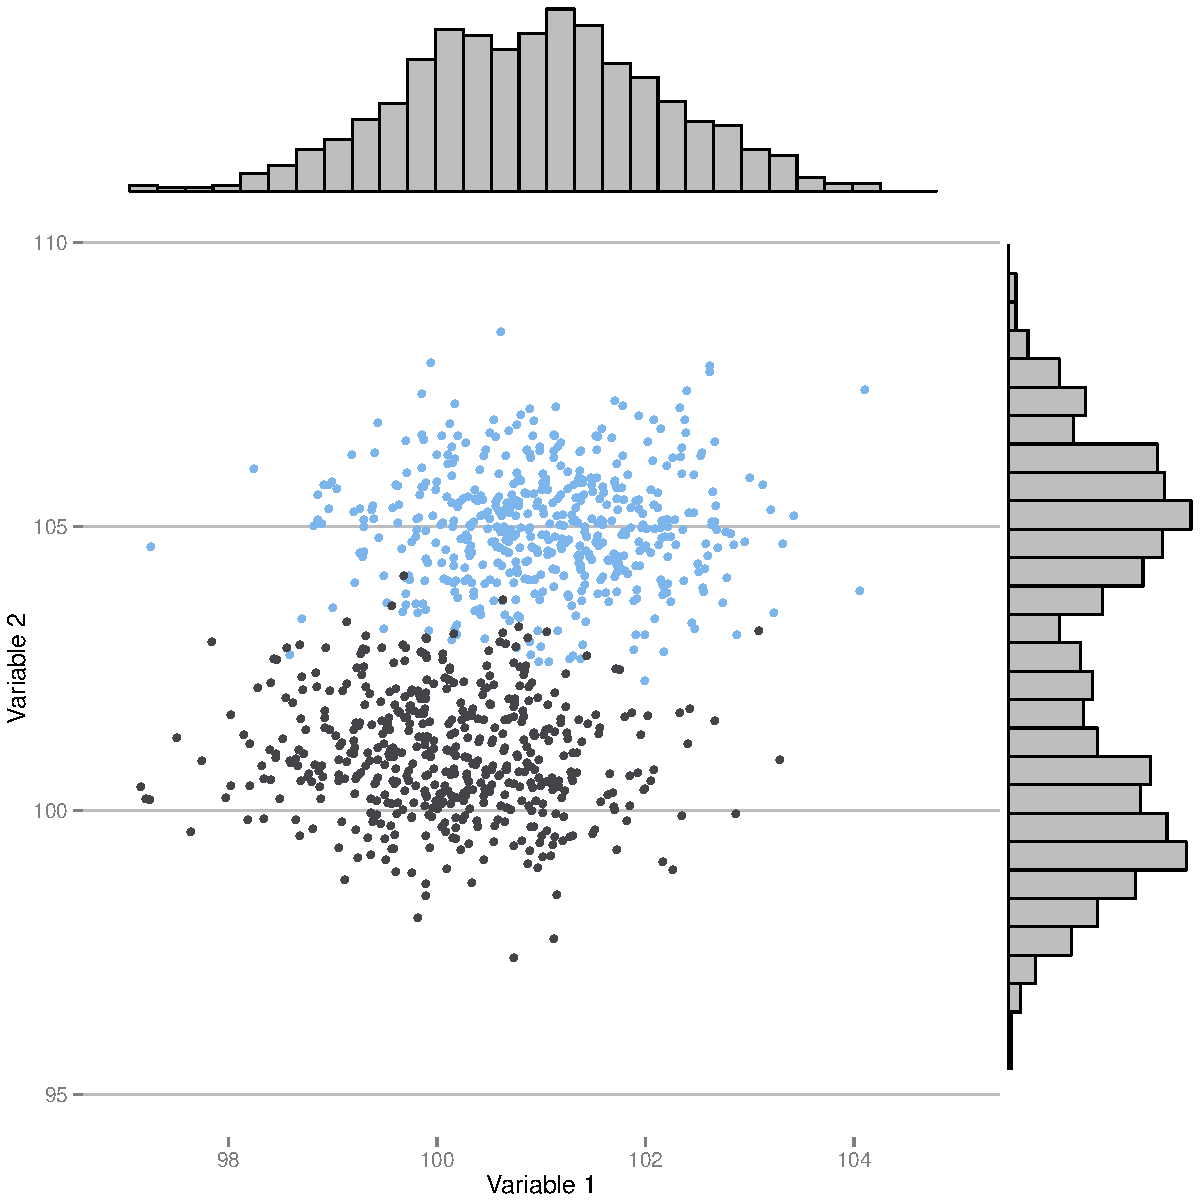
\includegraphics[scale=0.6]{graphics/ctmixtures/equifinality-variable-effect.pdf}
\caption{Simple example of the effect of variable choice in distinguishing models.  The variable on the X axis displays quite a bit of overlap between models, while the variable on the Y axis distinguishes the models with fairly high accuracy.}
\label{img:variables-equifinality-example}
\end{figure}

\begin{figure}[ht]
\centering
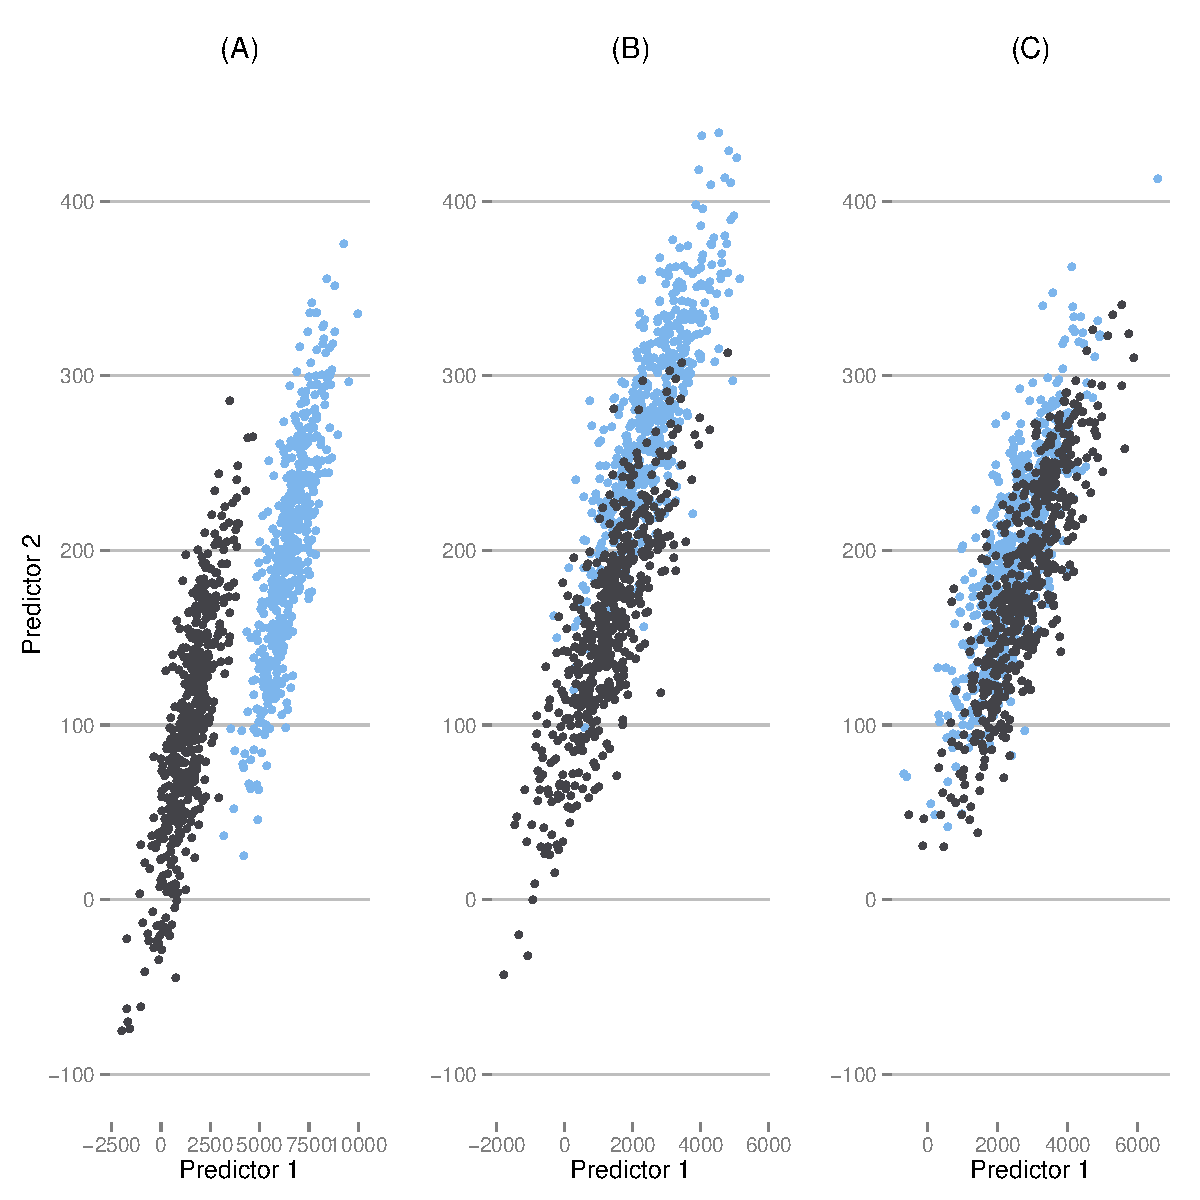
\includegraphics[scale=0.6]{graphics/ctmixtures/distributional-overlap.pdf}
\caption{Simple example of model outcomes with different degrees of distinguishability: (A) simulated data point from two fully separate models, (B) two models with a limited overlap region, (C) and two models whose outcomes are highly overlapping.}
\label{img:separability-example}
\end{figure}

\begin{figure}[ht]
\centering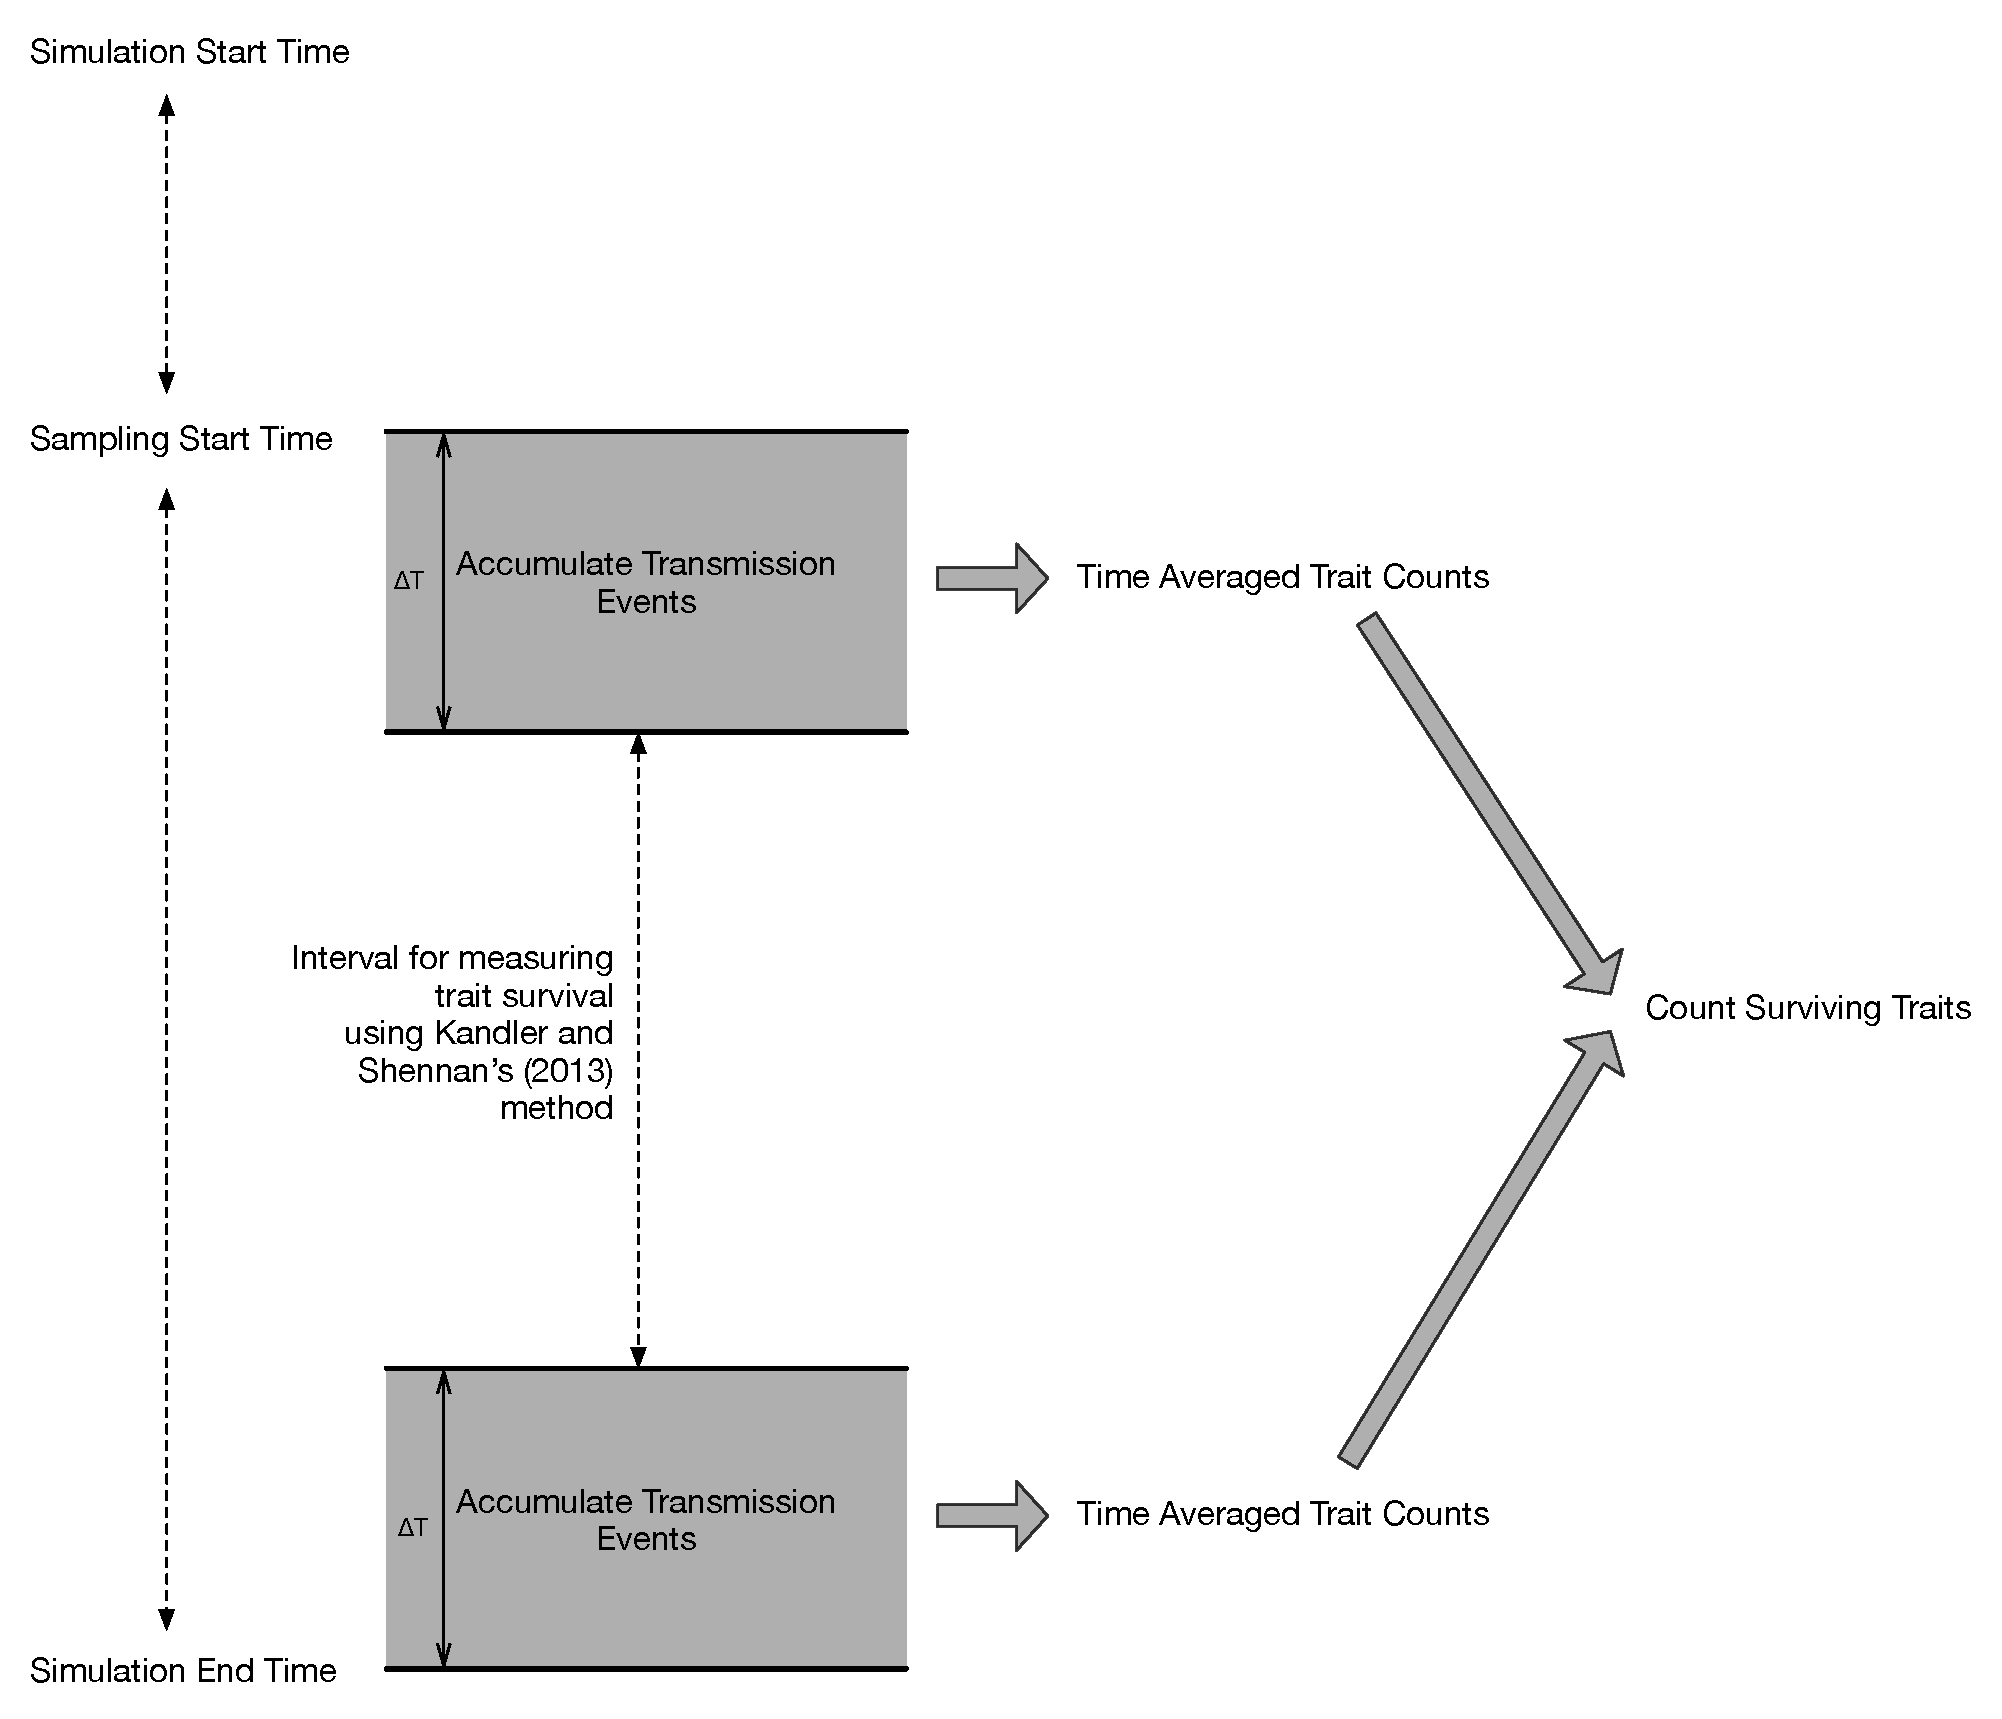
\includegraphics[scale=0.4]{graphics/ctmixtures/time-averaging-with-kandler-sampling.pdf}
\caption{Schematic of how trait survival as described by Kandler and Shennan \cite{kandler2013non} is extended to time averaged samples of transmission events.  Time runs from the start of the simulation run at the top, to the end at the bottom.  The interval of time over which we calculate the Kandler-Shennan trait survival is given as a simulation parameter, and represents the gap in the middle of the diagram.  Before and after that gap are sampling windows during which transmission events are accumulated over some number of simulated ``generations'' (values of 10, 25, 50, and 100 are used in this paper).  Trait survival is then calculated as the number of traits present in the starting time averaged sample of transmission events, which are still present in the ending time averaged sample of events.}
\label{img:timeaveraging}	
\end{figure}


% \begin{figure}[ht]
% \centering
% \includegraphics[scale=0.5]{figure/unbiased-biased-kappa-dotchart.pdf}
% \caption{Cohen's kappa for correctly predicting whether simulated data points originate from unbiased copying or any of 3 other biased transmission models.  High values of kappa correspond to high accuracy in correctly distinguishing between transmission models, while values well below 0.5 indicate great difficult and low classifier accuracy.  Each line in the dotchart represents a different data collection treatment, and overall the results indicate that significant equifinality exists except when time averaging is absent and a population census (or near equivalent) is available.}
% \label{img:unbiased-biased-kappa}
% \end{figure}

% \begin{figure}[ht]
% \centering
% \includegraphics[scale=0.5]{figure/unbiased-balbiased-kappa-dotchart.pdf}
% \caption{Cohen's kappa for correctly predicting whether simulated data points originate from unbiased copying or a balanced mixture of pro- and anti-conformist individuals.  Each line in the dotchart represents a different data collection treatment, and overall the results indicate that significant equifinality exists except when time averaging is absent and a population census (or near equivalent) is available.}
% \label{img:unbiased-biased-kappa}
% \end{figure}

% \begin{figure}[ht]
% \centering
% \includegraphics[scale=0.5]{figure/proanticomparison-kappa-dotchart.pdf}
% \caption{Cohen's kappa for correctly predicting whether simulated data points originate from a conformist-dominated mixed population versus a mixed population dominated by anti-conformists.  Each line in the dotchart represents a different data collection treatment, and overall the results indicate that strong equifinality exists regardless of the data collection treatment.}
% \label{img:proanti-kappa}
% \end{figure}



    
    \chapter{Combinatorial Structure of the Deterministic Seriation Method with Multiple Subset Solutions}
    \label{chap:seriationcombinatorics-paper}
    
\begin{description}[leftmargin=-1\labelwidth]
\item[\textsc{Abstract}] Seriation methods order a set of descriptions given some criterion (e.g., unimodality or minimum distance between similarity scores).  Seriation is thus inherently a problem of finding the optimal solution among a set of permutations of objects.  In this short technical note, we review the combinatorial structure of the classical seriation problem, which seeks a single solution out of a set of objects.  We then extend those results to the iterative frequency seriation approach introduced by \citet{Lipo1997}, which finds optimal subsets of objects which each satisfy the unimodality criterion within each subset.  The number of possible solutions across multiple solution subsets is larger than $n!$, which underscores the need to find new algorithms and heuristics to assist in the deterministic frequency seriation problem. 

\item[\textsc{Source}]  Posted to Arxiv.org (\url{https://arxiv.org/abs/1412.6060}), in December 2014.  Co-authored with Carl P. Lipo.
\end{description}


\section{Single Seriation Combinatorics}
\label{sec:single-seriation}

%%%%%%%%%%%%%%%%%%%%%%%%%%%%%%%%%%%%%%%%%%%%%%%%%%%%%%%%%%%%%%%%%%%%%%%%%%%%%

%%%%%%%%%%%%%%%%%%%%%%%%%%%%%%%%%%%%%%%%%%%%%%%%%%%%%%%%%%%%%%%%%%%%%%%%%%%%%

Seriation, whether employing class frequencies or simple occurrence to order assemblages, yields solutions which are permutations of the set of assemblages.  Because we cannot determine the ``polarity'' of a seriation solution---which ends represent early and late---from the class data alone, a unique seriation solution is thus formally a pair of mirror-image permutations:
\begin{equation}
\{a,d,b,c,e\} \equiv \{e,c,b,d,a\}
\end{equation}

This means that a set of $n$ assemblages can yield $n! / 2$ distinct solutions, regardless of whether solutions are composed of ordered similarity matrices or``Fordian'' frequency curves.  With small numbers of assemblages, enumeration and testing of all possible solutions is easy, even without parallel testing across many processors.  The ability to test solutions by enumeration quickly breaks down with only a modest number of assemblages.  Table \ref{tab:ss-stats} gives the number of unique solutions for selected problem sizes between 4 and 100 assemblages, and estimates of processing time to enumerate and test all solutions, assuming a cluster of 64 cores, and \ensuremath{5\times 10^{-4}} seconds per solution test.\footnote{These assumptions concerning per-trial processing time and parallelism are arbitrary but within reach of social scientists given Amazon's EC2 cloud computing infrastructure, without requiring formal ``supercomputer'' access.  Modification by a factor of 10 has little effect on the results, perhaps shifting feasibility upward slightly before combinatorial explosion occurs.}  With 10 assemblages, we can test all solutions quickly enough that even a serial algorithm on a single core will be adequate to find the global best solution in a matter of hours, with parallelism improving this to real time responses.  

%%%%%%%%%%%%%%%%%%%%%%%%%%%%%%%%%%%%%%%%%%%%%%%%%%%%%%%%%%%%%%%%%%%%%%%%%%%%%
% latex table generated in R 3.1.2 by xtable 1.7-4 package
% Mon Mar  2 09:12:21 2015
\begin{table}[ht]
\centering
\begin{tabular}{|c|r|r|r|}
  \hline
N & Seriation Solutions & Seconds & Years \\ 
  \hline
  4 &  12 & 9.4e-05 & 3e-12 \\ 
    6 & 3.6e+02 & 0.0028 & 8.9e-11 \\ 
    8 & 2e+04 & 0.16 & 5e-09 \\ 
   10 & 1.8e+06 &  14 & 4.5e-07 \\ 
   12 & 2.4e+08 & 1.9e+03 & 5.9e-05 \\ 
   13 & 3.1e+09 & 2.4e+04 & 0.00077 \\ 
   14 & 4.4e+10 & 3.4e+05 & 0.011 \\ 
   15 & 6.5e+11 & 5.1e+06 & 0.16 \\ 
   16 & 1e+13 & 8.2e+07 & 2.6 \\ 
   20 & 1.2e+18 & 9.5e+12 & 3e+05 \\ 
   40 & 4.1e+47 & 3.2e+42 & 1e+35 \\ 
   60 & 4.2e+81 & 3.3e+76 & 1e+69 \\ 
   80 & 3.6e+118 & 2.8e+113 & 8.9e+105 \\ 
  100 & 4.7e+157 & 3.6e+152 & 1.2e+145 \\ 
   \hline
\end{tabular}
\caption{Number of unique seriation solutions and parallel processing time for sets of assemblages $4 < n < 100$, testing solutions across 64 cores, assuming 5ms per trial} 
\label{tab:ss-stats}
\end{table}

%%%%%%%%%%%%%%%%%%%%%%%%%%%%%%%%%%%%%%%%%%%%%%%%%%%%%%%%%%%%%%%%%%%%%%%%%%%%%

A typical characteristic of many combinatorial algorithms is that small changes in problem size can have massive changes in processing time.  13 assemblages will turn out to be the practical limit for direct enumeration, even given parallel processing with circa-2012 technology, with total processing time of nearly 3 days running 64 cores at full capacity.\footnote{Realistically, almost nobody would contemplate doing this, given the expense of the computing time relative to the value of guaranteeing the optimal solution, but the hypothetical example demonstrates that such solutions are \emph{feasible}.}  Problems involving 14 and 15 assemblages reach the point where large clusters require more than a month and 19 months respectively, to solve.  Beyond 15 assemblages, a ``combinatorial explosion'' sets in, with 20 assemblages requiring more than 3 million years, before solution times quickly exceed the lifetime of the universe.  

In short, top-down enumerative methods are feasible for small sets of assemblages, and given widespread availability of multiple core computers, seriation packages should employ enumeration for small problems, or to build and test smaller parts of larger seriation solutions.  

\section{Deterministic Seriation with Multiple Solution Groups}
\label{sec:seriation-groups}

%%%%%%%%%%%%%%%%%%%%%%%%%%%%%%%%%%%%%%%%%%%%%%%%%%%%%%%%%%%%%%%%%%%%%%%%%%%%%

%%%%%%%%%%%%%%%%%%%%%%%%%%%%%%%%%%%%%%%%%%%%%%%%%%%%%%%%%%%%%%%%%%%%%%%%%%%%%   "

In an earlier paper \citep{Lipo1997}, we introduced an iterative method for finding deterministic solutions to the frequency seriation problem by partitioning assemblages into subsets, each of which meets the unimodal ordering principle, within tolerance limits governed by sample size.  \citet{Lipo2001} extended and refined the method in his dissertation research.  Our initial work on the method employed a combination of automated calculations (e.g., bootstrap significance tests for pairwise orderings), and manual sorting of assemblages into groups and specific positions (using an Excel macro package available at \url{http://lipolab.org/seriation.html}).  Figure \ref{fig:mult-seriation-groups} is an example of seriation with multiple solution groups, from Lipo's dissertation research in the Lower Mississippi Valley.  

\begin{figure*}
	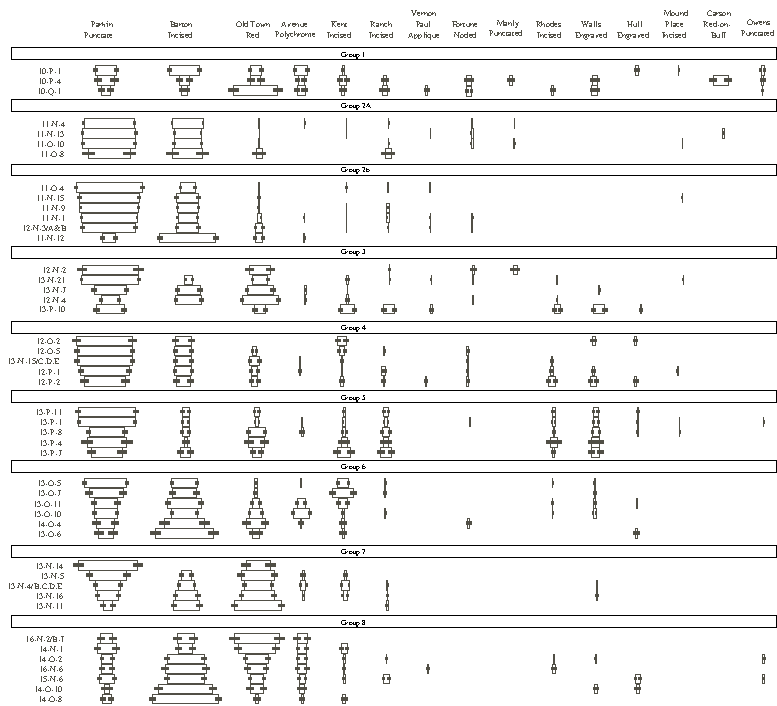
\includegraphics[scale=0.75]{graphics/seriationcombinatorics/lipo-figure-4-4.pdf}
	\caption{Example of a deterministic frequency seriation with assemblages partitioned into multiple subsets or solution groups.  From \citet{Lipo2001}, Figure 4.4.}
	\label{fig:mult-seriation-groups}
\end{figure*}

Our initial work suggests assemblages seriate together into groups reflecting variation in the intensity of \ct among assemblages, over their duration of accumulation. In most cases, solution groups tend to be spatiotemporally compact, and form clusters when mapped on the landscape, although long-distance connections between past communities can also yield patterns which are more complex and less cohensive when mapped.  Madsen's dissertation research is aimed at tying the properties seriation solution groups to their causes in regional patterns of interaction and the dynamics of specific \ct models.  

%%%%%%%%%%%%%%%%%%%%%%%%%%%%%%%%%%%%%%%%%%%%%%%%%%%%%%%%%%%%%%%%%%%%%%%%%%%%%
% latex table generated in R 3.1.2 by xtable 1.7-4 package
% Mon Mar  2 09:12:21 2015
\begin{table}[ht]
\centering
\begin{tabular}{|c|r|r|r|}
  \hline
\# of Solution Groups (m) & 20 & 40 & 60 \\ 
  \hline
  3 & 5.8e+08 & 2e+18 & 7.1e+27 \\ 
    4 & 4.5e+10 & 5e+22 & 5.5e+34 \\ 
    6 & 4.3e+12 & 1.8e+28 & 6.8e+43 \\ 
    8 & 1.5e+13 & 3.2e+31 & 3.8e+49 \\ 
   10 & 5.9e+12 & 2.4e+33 & 2.7e+53 \\ 
   15 &  & 2.9e+34 & 2.2e+58 \\ 
   20 &  & 1.6e+32 & 1.7e+59 \\ 
   25 &  &  & 3.7e+57 \\ 
   30 &  &  & 9.6e+53 \\ 
   \hline
\end{tabular}
\caption{Number of ways to form m subsets (seriation solutions) from 20, 40, and 60 assemblages} 
\label{tab:subsets}
\end{table}

%%%%%%%%%%%%%%%%%%%%%%%%%%%%%%%%%%%%%%%%%%%%%%%%%%%%%%%%%%%%%%%%%%%%%%%%%%%%%

In this section, the goal is to understand the complexity of the multiple seriation groups problem, constructing reasonable upper bounds for a given problem size, even if some problems encountered in real analyses do not approach the worst case.  From a combinatorial standpoint, seriation with multiple solution groups has the following structure.  
We begin with $n$ assemblages in total, and seek a solution or solutions whereby we end up with $m$ solution groups, where $m < n$.  Each solution must have at least one assemblage, and in practice will often have 3 or more (singletons may indicate assemblages which simply do not ``fit'' with anything else in the data set).  The number of ways that $n$ objects can be partitioned into $m$ non-empty subsets (or solution groups) is given by the Stirling numbers of the second kind, which are given by the recursion equation:
\begin{equation}
\stirlingsubset{n}{m} = m \stirlingsubset{n-1}{m} + \stirlingsubset{n-1}{m-1}
\end{equation}
Table \ref{tab:subsets} gives the number of ways to form a specific number of subsets (or seriation solution groups) from sets of assemblages ranging from 20 to 60.  Each column runs from 3 solution groups to half of the number of assemblages, since the number of possible subsets is maximized just before $n/2$ and declines thereafter (Figure \ref{fig:subsets-graph}).  

%%%%%%%%%%%%%%%%%%%%%%%%%%%%%%%%%%%%%%%%%%%%%%%%%%%%%%%%%%%%%%%%%%%%%%%%%%%%%
\begin{figure*}
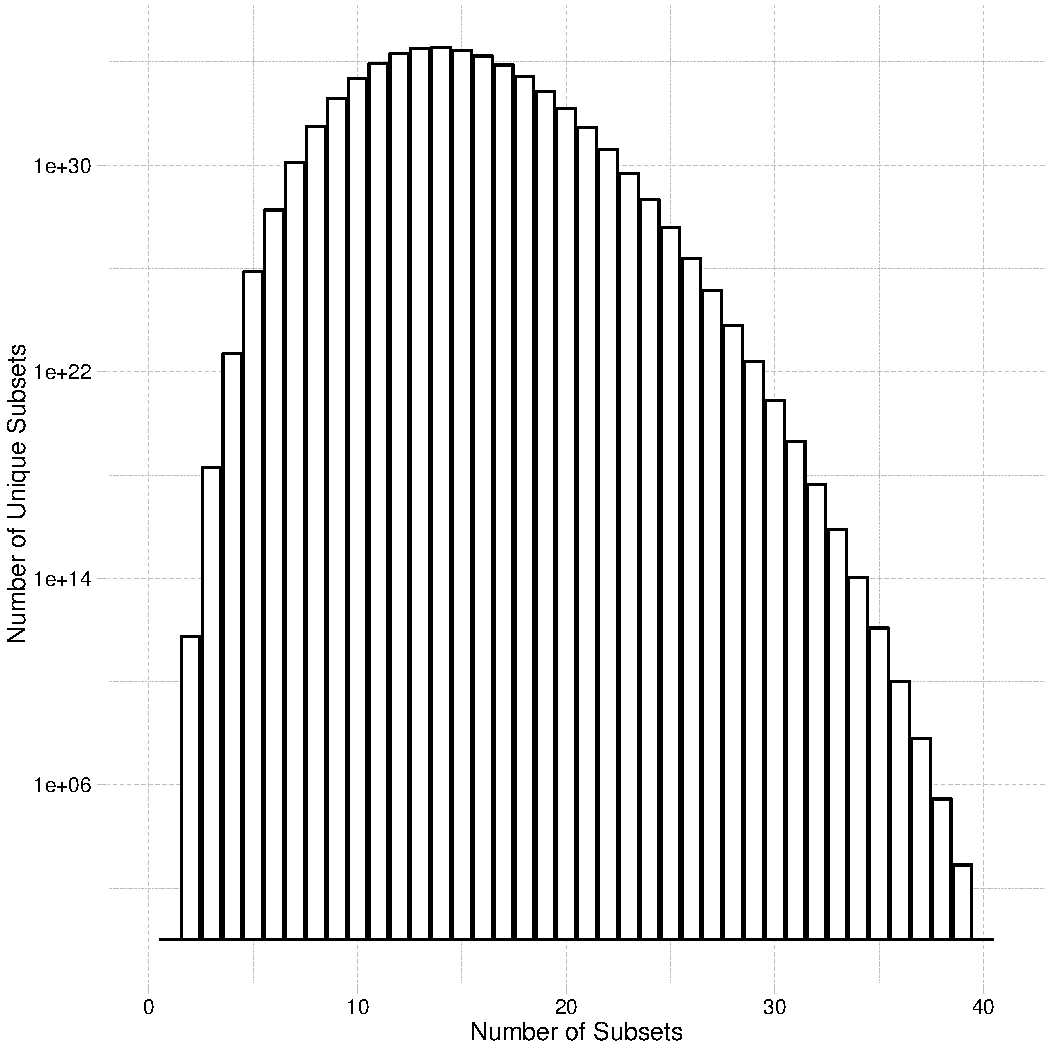
\includegraphics[width=3.5in]{graphics/seriationcombinatorics/subsets-graph-1.pdf} \caption[Number of Unique Solution Sets for 40 Assemblages When Partitioned Into ]{Number of Unique Solution Sets for 40 Assemblages When Partitioned Into $m$ Solution Groups\label{fig:subsets-graph}}
\end{figure*}


%%%%%%%%%%%%%%%%%%%%%%%%%%%%%%%%%%%%%%%%%%%%%%%%%%%%%%%%%%%%%%%%%%%%%%%%%%%%%

We can immediately see that there are an enormous number of possible subsets for any assemblage size.  There are fewer subsets, of course, than complete permutations of the set of assemblages since subsets are unordered (i.e., $\stirlingsubset{n}{m} < n! \,\mathrm{for\,all }\,m$).  However, in the multiple seriation group problem, the problem size is larger than the corresponding Stirling number because we do not know in advance how many groups (subsets) a set of assemblages will seriate into.  Thus, the total number of unique subsets which might contain the optimal solution is the total of the number of subsets, across all subset sizes:
\begin{equation}
\sum_{i=1}^n \stirlingsubset{n}{i}
\label{eq:sum-stirling}
\end{equation}
This result is still smaller than the total permutations for a set of $n$ assemblages.  For example, given 40 assemblages, $n! = 8.159\e{47}$, whereas the total from Equation \ref{eq:sum-stirling} for 40 assemblages is $1.575\e{35}$.  

Another factor to consider is that each of these unique subsets resulting from a partition of $n$ assemblages into seriation groups is still unordered.  For example, if we partition 10 assemblages into 3 solution groups, there are 9330 unique ways of assigning the 10 assemblages to the 3 solution groups.  Each group within a partition will have $n_i$ members, where $\sum n_i = n$.   The number of unique seriations for each of the 3 solution groups is $n_i ! / 2$, but we cannot assume that solution groups will have a balanced or equal number of assemblages (as Figure \ref{fig:mult-seriation-groups} does).  Partitions such as:
\begin{equation*}
\{1,2,3,4,5,6\} \{7,8\} \{9,10\}  
\end{equation*}
are common in seriating real assemblages \citep{Lipo2001}.   

%%%%%%%%%%%%%%%%%%%%%%%%%%%%%%%%%%%%%%%%%%%%%%%%%%%%%%%%%%%%%%%%%%%%%%%%%%%%%

%%%%%%%%%%%%%%%%%%%%%%%%%%%%%%%%%%%%%%%%%%%%%%%%%%%%%%%%%%%%%%%%%%%%%%%%%%%%%


%%%%%%%%%%%%%%%%%%%%%%%%%%%%%%%%%%%%%%%%%%%%%%%%%%%%%%%%%%%%%%%%%%%%%%%%%%%%%

%%%%%%%%%%%%%%%%%%%%%%%%%%%%%%%%%%%%%%%%%%%%%%%%%%%%%%%%%%%%%%%%%%%%%%%%%%%%%


Since the factorial function grows so quickly, the computational cost of determining the correct permutation within a given seriation solution group is controlled by the size of the largest subset, especially if the other subsets are relatively small, as in the previous example.  At worst, for a solution set with $m$ solution groups, $m-1$ solution groups will contain 1 assemblage each, and the last solution group will consist of the remaining $n-m-1$ assemblages.  This means, of course, that the worst case would involve consideration of on the order of $(n-m-1)!$ permutations within each solution group, for each of the subsets given by Equation \ref{eq:sum-stirling}.  This yields:
\begin{equation}
\sum_{m=1}^n \stirlingsubset{n}{m} (n-m-1)!
\end{equation}
Table \ref{tab:total-mult} gives the total number of possible solutions for assemblages ranging from 4 to 100, where solutions may fall into multiple seriation groups of any size.  

%%%%%%%%%%%%%%%%%%%%%%%%%%%%%%%%%%%%%%%%%%%%%%%%%%%%%%%%%%%%%%%%%%%%%%%%%%%%%
% latex table generated in R 3.1.2 by xtable 1.7-4 package
% Mon Mar  2 09:12:22 2015
\begin{table}[ht]
\centering
\begin{tabular}{|c|r|r|r|}
  \hline
N & Total Solutions & Seconds & Years \\ 
  \hline
  4 &  15 & 0.00012 & 3.7e-12 \\ 
    6 & 4.7e+02 & 0.0037 & 1.2e-10 \\ 
    8 & 5.2e+04 & 0.4 & 1.3e-08 \\ 
   10 & 1.5e+07 & 1.1e+02 & 3.6e-06 \\ 
   12 & 8.5e+09 & 6.6e+04 & 0.0021 \\ 
   13 & 2.6e+11 & 2e+06 & 0.064 \\ 
   14 & 8.9e+12 & 7e+07 & 2.2 \\ 
   15 & 3.5e+14 & 2.8e+09 &  87 \\ 
   16 & 1.6e+16 & 1.2e+11 & 3.9e+03 \\ 
   20 & 1.7e+23 & 1.3e+18 & 4.2e+10 \\ 
   40 & 9e+65 & 7e+60 & 2.2e+53 \\ 
   60 & 5.1e+116 & 4e+111 & 1.3e+104 \\ 
   80 & 5.1e+172 & 4e+167 & 1.3e+160 \\ 
  100 & 4.4e+232 & 3.4e+227 & 1.1e+220 \\ 
   \hline
\end{tabular}
\caption{Number of total solutions with multiple seriation groups and processing time for sets of assemblages 4 < n < 100, testing solutions across 64 cores} 
\label{tab:total-mult}
\end{table}

%%%%%%%%%%%%%%%%%%%%%%%%%%%%%%%%%%%%%%%%%%%%%%%%%%%%%%%%%%%%%%%%%%%%%%%%%%%%%




\section{Discussion}
\label{sec:conclusions}

Clearly, in the worst case, the combinatorial complexity of the multiple seriation groups problem is much worse than even the straight factorial case involved in single solution permutations.  The feasibility of parallelized enumerative methods still explodes after 13 assemblages, but much more steeply.  The goal of a new algorithm for deterministic multiple group seriations is, therefore, to employ heuristics to drastically reduce the size of the solution space.  Vast amounts of the solution space involve partial orders which violate unimodality, but of course we cannot easily identify those regions of solution space \emph{a priori} without testing possibilities.  But given small partial solutions which do meet the seriation model, we can easily test solutions which are ``adjacent'' to the partial solutions, suggesting that agglomerative heuristics may be the best approach to finding a computationally feasible method.  



    
    \chapter{Measuring Cultural Relatedness Using Multiple Seriation Ordering Algorithms}
    \label{chap:multipleseriation-paper}
    \begin{description}[leftmargin=-1\labelwidth]
\item[\textsc{Abstract}] Seriation is a long-standing archaeological method for relative dating that has proven effective in probing regional-scale patterns of inheritance, social networks, and cultural contact in their full spatiotemporal context. The orderings produced by seriation are produced by the continuity of class distributions and unimodality of class frequencies, properties that are related to social learning and transmission models studied by evolutionary archaeologists. Linking seriation to social learning and transmission enables one to consider ordering principles beyond the classic unimodal curve. Unimodality is a highly visible property that can be used to probe and measure the relationships between assemblages, and it was especially useful when seriation was accomplished with simple algorithms and manual effort. With modern algorithms and computing power, multiple ordering principles can be employed to better understand the spatiotemporal relations between assemblages. Ultimately, the expansion of seriation to additional ordering algorithms allows us an ability to more thoroughly explore underlying models of cultural contact, social networks, and modes of social learning. In this paper, we review our progress to date in extending seriation to multiple ordering algorithms, with examples from Eastern North America and Oceania.

\item[\textsc{Source}]  Submission to Electronic Symposium, ``Evolutionary Archaeologies: New Approaches, Methods, And Empirical
Sufficiency'' at the Society for American Archaeology conference, April 2016  Co-authored with Carl P. Lipo.  
\end{description}

%%%%%%%%%%%%%%%%%%%%%%%%%%%%%%%%%%%%%%%%%%%%%%%%%%%%%%%%%%%%%%%%%%%%%%%%%%%%%%%%%%%%%%%%%

\section{Introduction}\label{introduction}

Seriation is a set of methods that uses patterns in the occurrence or
abundance of historical classes to construct an ordering among otherwise
unordered assemblages or objects \citep{Dunnell:1970aa}. Its early 20th
century developers built seriation as a relative dating method and
orders constructed by seriation were intended to be chronological
\citep{o2000applying, o1998james, Lyman:2006aa, OBrien1999b, lyman1997rise}.
While practitioners such as James Ford
\citep{Ford:1938aa, Phillips1951, Ford:1935aa} noted that seriation
techniques also create orderings which incorporate the effects of
spatial variation in addition to temporal change, the dominant use of
seriation in archaeology has been to build chronology.

As a chronological tool, seriation has been success in developing an
understanding the large-scale temporal structure of the archaeological
record in the New World
\citep{Beals1945, Bluhm1951, Evans1955, Ford1949, Kidder1917, Mayer-Oakes1955, Meggers1957, Phillips1951, Rouse1939, Smith1950}.
Despite this success, the method has largely been ignored since the
advent of radiocarbon dating given its primary association as a relative
dating method. But seriation is only a dating method in the sense that
chronology is one possible inference that can be obtained by mapping the
spatiotemporal pattern of change in cultural variants. Other inferences
are possible, and in particular, there is a growing understanding that
seriation is one of several methods for documenting the evolutionary history of
past populations
\citep{Lipo1997Population,Lipo2000, Lipo2001,Lipo2001a,Lipo2005,lipomadsen1997,lipomadsendunnell2015,Neiman1995,OBrien1999b,Teltser1995}.

Seriation is based on the notion that the frequencies of classes of
artifacts reflect heritable continuity when it arises from information
being passed between populations over time; that is, from cultural
transmission processes. Although the fact that seriation, in some sense,
measures cultural transmission has been implicit since the earliest
discussions of the method \citep[e.g.,][]{Kroeber1923}, the connection
remained a common sense generalization until the mid 1990's. Fraser
Neiman \citeyearpar{Neiman1990}, in his dissertation and later his seminal
  article \citep{Neiman1995}, noted that the unimodal patterns that
form the core of the traditional frequency seriation technique are
regularly seen in the trajectories seen when simulating unbiased
transmission. In order to make this connection both rigorous and useful
in empirical work, we began a research program aimed at exploring the
connection between cultural transmission models and seriation methods
\citep{Lipo1997Population}. Our investigation into seriation has
resulted in numerous publications, new seriation software algorithms,
and many conference papers
\citep{Lipo2008, Lipo2001neutrality, Lipo2001a, Lipo2005, lipomadsen1997, lipomadsendunnell2015, Madsen2014, madsenlipo2015b, Madsen2008, o2015design}.

The core of the all seriation techniques are a set of ``ordering
principles'' which describe how the data points making up each
assemblage or object are rearranged in order to achieve a valid
seriation solution. Traditionally, there are two principles: occurrence
and frequency \citep{Dunnell:1970aa, Rouse1967, Whitlam:1981vs}. The
``occurrence principle'' states that a valid ordering leaves no temporal
gaps in the distribution of the historical classes used, and thus that
temporal orders are continuous
\citep{dempsey1963statistical, rowe1959archaeological}. The
``frequency'' or ``popularity'' principle states that in a valid
ordering, the frequencies making up the continuous distribution of each
historical type will be unimodal, possessing a single peak of
``popularity'' \citep{Nelson1916}.

\begin{figure}[ht]
\centering
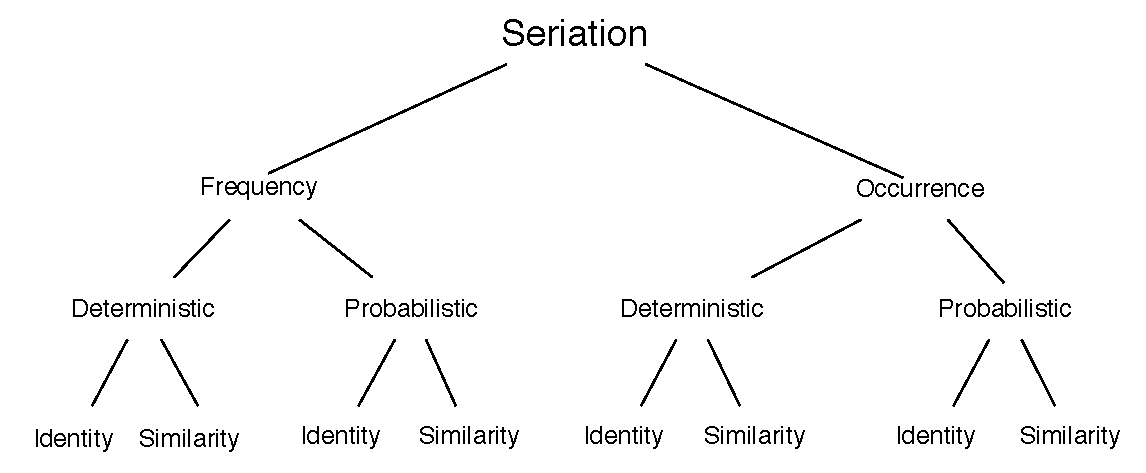
\includegraphics[scale=0.6]{graphics/multipleseriation/seriation-methods.pdf}
\caption{\citet{Dunnell1981} defines seriation to be a set of methods which use historical classes to chronologically order otherwise unordered archaeological assemblages and/or objects. Historical classes are those which display more variability through time than through space. Occurrence seriation uses presence/absence data for each historical class from each assemblage \citep{Kroeber1916,Petrie:1899aa}. Frequency seriation uses ratio level abundance information for historical classes \citep{Spier1917,Ford:1935aa,Ford:1962aa}. Frequency and occurrence seriation techniques can take the form of deterministic algorithms that require an exact match with the unimodal model or probabilistic algorithms that accept departures from an exact fit. Identity approaches employ raw data (whether frequency or occurrence) to perform the ordering. Similarity approaches transform the raw data into a non-unique coefficient (e.g., Brainerd Robinson, squared Euclidean distance); the coefficients then form the basis for ordering.}
\label{img:seriation-methods}
\end{figure}

Both the frequency and occurrence principle work to sort descriptions of
assemblages through time. The robustness of methods built on these
principles is easily demonstrated by the continued utility of the basic
chronological frameworks erected by culture historians in the first half
of the 20th century using seriation along with stratigraphy and marker
types \citep{lyman1997rise}. It is intriguing to note, however, that the
frequency principle remains an empirical generalization that is only
suggested by the \emph{generalized} behavior of cultural transmission models.  Unimodality is not a necessary consequence. 
From Neiman's simulations
\citep[i.e.,][]{Neiman1995}, one can see that the results of cultural
transmission are not strictly or necessarily unimodal. This possibility
suggests to us that seriation as a method requires further
methodological development, especially if it is to be one of our major
tools in tracing historical and heritable continuity in the
archaeological record.\footnote{Cladistics and phylogenetic methods,
  especially those which take into account temporal differences in the
  samples being studied (stratocladistics) and which are capable of
  yielding phylogenetic networks in addition to trees, are the other
  major tools by which we can measure heritable and historical
  continuity.}

In this paper, we explore an alternative to unimodality and the
``popularity principle'' that drives classical frequency seriation:
exact minimization of inter-assemblage distance metrics, or
``continuity'' seriation. Although not a new principle, it was
underappreciated especially prior to the contemporary explosion of
computing power. We demonstrate that an exact form of distance
minimization, in contrast to the statistical or approximate minimization
associated with multidimensional scaling, generates solutions that are
usually identical to the application of unimodality to the same data.
Furthermore, using simulated data, we examine situations where frequency
and continuity seriations may differ in minor ways, without affecting
the overall ordering of the data set. Although there is still great
value in the classical approach, the advantage of developing new
seriation approaches is that we can often apply distance minimization to
classes and types which do not necessarily display the classical
unimodal form, which opens seriation to wider classes of data. In
addition, distance minimization can be formulated within large scale,
parallel machine learning frameworks, and thus made applicable to large
data sets, increasing our ability to examine regional scale phenomena in archaeology, and making seriation useful for detailed analysis of contemporary data sets which dwarf the sample sizes typically available to archaeologists.

\section{Seriation and the Frequency
Principle}\label{seriation-and-the-frequency-principle}

Seriation, in the Americanist sense, was initially developed by Alfred
Kroeber \citep{Kroeber1916} in the Southwest, based on his observations
of changes in the relative abundance of forms of ceramic decorations
found on sherds located in assemblages near Zuni Pueblo. The primitive
seriation proposed by Kroeber was quickly amended by Leslie Spier,
Alfred V. Kidder and Nels C. Nelson all of whom were conducting
stratigraphic excavations in the American Southwest
\citep{Kidder1917, Nelson1916, Spier1917}. This group of researchers all
noticed that when ceramics were described in a particular way -- called
``stylistic'' by Kidder \citeyearpar{Kidder1917} -- the temporal
distribution of the types took the form of ``normal curves.'' Using such
types, it was apparent that a series of assemblages collected from the
surface or otherwise undated could be arranged in chronological order by
rearranging them so that all type distributions approximated ``normal
curves'' simultaneously. The orders constructed in this way could also
be tested by finding stratified deposits and were found to be correct.
The resulting method then went on to dominate archaeological practice
for much of the next 50 years \citep{lyman1997rise}.

As powerful as seriation proved to be, these early formulations were
entirely intuitive and based on the generalization that greater temporal
differences between assemblages caused larger differences between
frequencies of decorated types, and that properly constructed historical
types displayed a clear pattern of change \citep[p.~220]{Phillips1951}:

\begin{quote}
If our pottery types are successful measuring units for a continuous
stream of changing cultural ideas, it follows that when the relative
popularity of these types is graphed through time, a more or less long,
single-peak curve will usually result. Put in another way, a type will
first appear in very small percentages, will gradually increase to its
maximum popularity, and then, as it is replaced by its succeeding type,
will gradually decrease and disappear.
\end{quote}

This compactly describes the ``popularity principle,'' originally
articulated by Nelson \citeyearpar{Nelson1916} and Wissler
\citeyearpar{wissler1916application}. A key word in the above is
``usually,'' since not all types display the unimodal distribution
described, even when the attributes chosen are explicitly stylistic and
decorative. Types suitable for frequency seriation were a subset of
stylistic variation, comprising those which displayed spatial and
temporal contiguity, a long enough duration that the types overlapped in
their representation among sites and assemblages, and those whose
distribution through time displayed the characteristic unimodal form
which allowed the analyst to arrange them by eye. Culture historians
also minimized the effect of chance and potential recurrence by
insisting that the classes used for measurement were constructed from
multiple dimensions \citep{Phillips1951, Lipo2001}. The overall process
of constructing and testing such types became known, after Krieger
\citeyearpar{Krieger1944}, as applying the ``test of historical
significance.''

\subsection{Unimodality and Cultural Transmission
Processes}\label{unimodality-and-cultural-transmission-processes}

In most cases (such as the above quote from Phillips, Ford, and
Griffin), the popularity principle is simply assumed to hold in
culture-historical applications. It is clear that culture historians
assumed that what generates heritable continuity, and thus allows the
tracing of chronological relations, is cultural transmission. As Lyman
\citeyearpar{lyman2008cultural} documents in careful detail, early 20th century
anthropology and archaeology understood and discussed a variety of
transmission processes informally, as generating the patterns they
studied, even if they used different terms and did not form quantitative
models for it. Rouse \citeyearpar{Rouse1939}, for example, explicitly
discussed the diffusion of cultural traits, in terms that we now
recognize as a spatiotemporal model of transmission. Kroeber, the father
of frequency seriation, clearly understood the connection between his
previous work and trait diffusion \citep{kroeber1937diffusion}. Deetz
and Dethlefsen \citetext{\citeyear{Deetz1965a}; \citeyear{Deetz1971}}
noted the spatial dimension to trait diffusion. There are many more
examples \citep{lyman2008cultural}.

Interest in studying cultural transmission in an explicit way has a long
history in archaeology. Since the 1970s, archaeologists have worked with
models of diffusion, with those models becoming increasingly
quantitative, statistical, and even explicitly mathematical
\citep[e.g.,][]{ammerman1971measuring}. These models of diffusion,
however, tended to be deterministic, especially those stemming from the
interdisciplinary literature on the diffusion of innovations
\citep[e.g.,][]{Rogers2003}. Deterministic models, however, ignore the
essential historically contingent pathways of culture transmission that
produce the patterns noted by culture historians as historically
significant. More recently archaeologists have become interested in
developing models for individual social learning events (see discussion in Chapter \ref{chap:ctmixtures-paper}. 

It was not until archaeologists began working with stochastic models of
cultural transmission, however, that we could easily visualize the sheer
variety of patterns that cultural transmission processes can, and do,
generate. Stochastic models of transmission allow us to easily explore
the precise conditions under which unimodal distributions occur in type
frequencies, what classification methods tend to produce it, and what
dimensions of variation combine to produce mostly unimodal behavior.

Dunnell's \citeyearpar{Dunnell1978} exposition of style as neutral
variation was one key step in the adoption of stochastic models of drift
from population genetics as the main tool for exploring cultural
transmission dynamics. Neiman \citeyearpar{Neiman1995} took this step
substantially further when he simulated drift in cultural variants as an
unbiased transmission process, as shown in Figure \ref{img:neiman-fig2}.
Immediately apparent is the fact that some variants do display unimodal
patterns, but most variants are multimodal or display violations of
unimodality at small scales even if the macroscopic shape seems to
conform to the popularity principle.

\begin{figure}[ht]
\centering
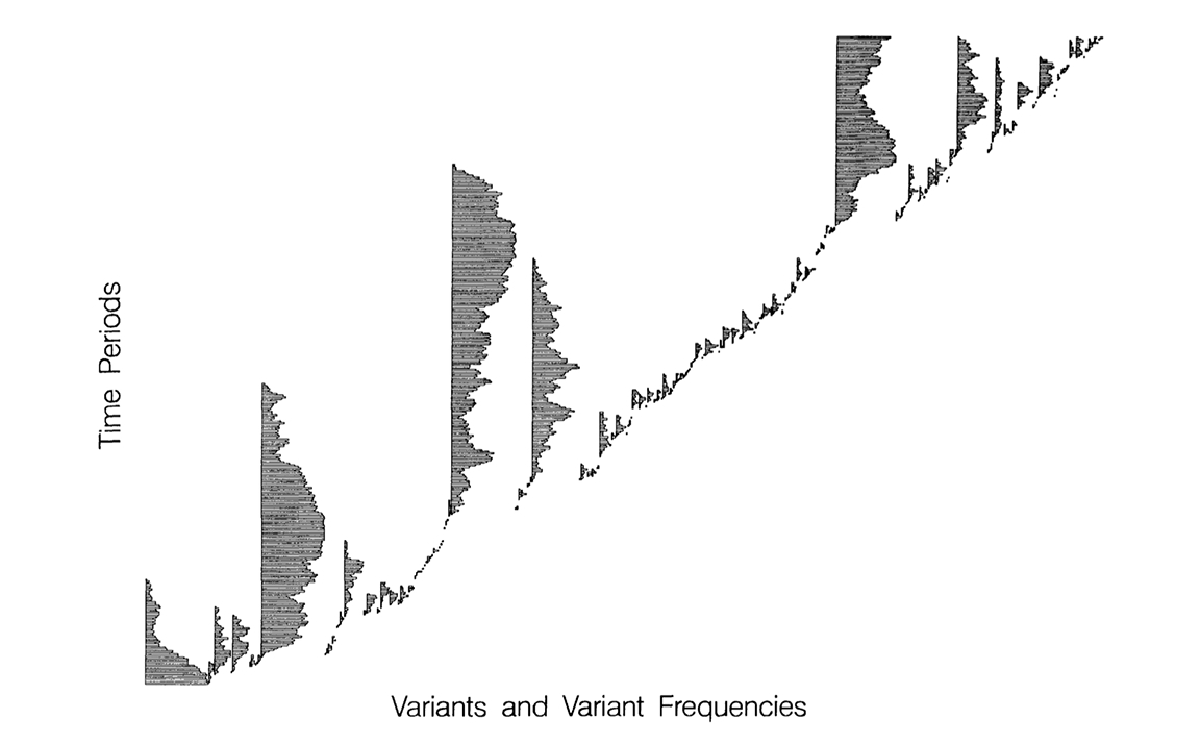
\includegraphics[scale=0.6]{graphics/multipleseriation/neiman-1995-figure2a.pdf}
\caption{Neiman's simulation of drift in cultural variant frequencies under unbiased cultural transmission (reproduction of Figure 2a from Neiman 1995.)}
\label{img:neiman-fig2}
\end{figure}

Figure \ref{img:neiman-fig2} shows that there is nothing
necessary about unimodality given cultural transmission.  Instead, culture-historical 
classifications and typologies were constructed such that they produced compact
spatiotemporal distributions and generally followed unimodal histories.  This is precisely
what Krieger's \citeyearpar{Krieger1944} ``test of historical significance'' yields when applied to a candidate
typology.
This is accomplished by ensuring that types are composed of multiple
dimensions of variation which co-occur on artifacts identified to that
type.  Each dimension of variation (e.g., surface treatment) may have complex histories,
like those seen in Figure \ref{img:neiman-fig2}, but when we combine several dimensions into a class, 
the history of the \emph{co-occurrence} of each combination of attributes becomes smoother and more 
localized in time and space.  This process of class construction necessarily results in a 
more compact spatiotemporal distribution for the class than for any of its constituent attributes.

Unimodality further arises from the constructed classes by examining their \emph{relative} frequency over time, expressed 
in percentages or fractions, which sum to 100\% or 1.0.  The latter constraint, which causes some combinations to be 
relatively less numerous when others increase in prevalence, smooths the more complex variation of individual attributes
into the histories of ``popularity'' that early twentieth century anthropologists noted \citeeg{Nelson1916,wissler1916application}.  

Taken together, these factors seem to explain why the intuitive
construction of historical types, from the continuous flow of the
products of cultural transmission processes, worked to produce
chronology through application of the common-sense popularity principle,
and why not all artifact classes constructed from otherwise
``stylistic'' dimensions of variation, are suitable for frequency
seriation using unimodality as the ordering criterion. From the
perspective of culture historians, unimodality was a sufficient criteria
for recognizing patterns that were likely chronological from those that
were likely not. While focusing on only those classes that produced
unimodal distributions in class frequencies might have ignored other
potentially historical significant classes, without any other means of
identifying chronological patterns, culture historians were satisfied
with the subset that worked.

\subsection{Continuity: An Alternative to
Unimodality}\label{continuity-an-alternative-to-unimodality}

There are several reasons why we should explore alternatives to
unimodality as an ordering algorithm for frequency seriation. First,
from a performance perspective, searching for unimodal orders is
computationally expensive, even for relatively small data sets
\citep{Madsen2014}. Even with the iterative, agglomerative method that
we introduced recently \citep{lipomadsendunnell2015}, the computation
time can grossly exceed computing capacity for data sets as small as 30.
While 30 is a large number of assemblages by most archaeological
standards especially when adequate sample size requirements are met, it
is a serious limitation. Without good techniques and ordering principles
seriation may not scale to much larger problems, and even be applicable
to the flood of data seen in modern day life.

Second, and more importantly from a theoretical perspective, it is
important to be able to trace heritable continuity even if does not
display a particular type of temporal frequency distribution. Using
traditional type construction methods and the test of historical
significance, culture historians were able to find \textbf{enough}
conforming types and classes to construct regional chronologies. The
goal of culture historians was to build chronologies using the most
efficient means possible to do so, not study combinations of trait
transmission through time and space. The use of seriation as a method
for tracing evolutionary relationships is a more demanding task than
establishing rough chronology in a region. Thus, it is worth searching
for additional ordering principles that may be useful for seriating more
classes of cultural variants. Specifically, there is strong relationship
between the number of classes in a seriation, and our ability to map
differences across space and time. We need methods that can evaluate
arbitrary sets of classes to arrive at the most detailed understanding
of cultural transmission landscapes (see Chapter \ref{chap:computational-metapopulation}).

A theoretically sound ordering principle for seriation should be
derivable from characteristics of the underlying cultural transmission
processes that we believe drive the spatiotemporal variation seriation
measures. Formal models of cultural transmission, such as those
formulated by Boyd and Richerson, Cavalli-Sforza and Feldman, and
borrowed from population genetics
\citep{Boyd1985, Cavalli-Sforza1981, Neiman1995} provide a good starting
place. Their models incorporate stochastic autoregressive processes in
which the probability distribution of outcomes at a given time are
dependent upon the outcomes from the immediate past. Mathematically,
then we can treat cultural transmission models as Markov processes,
usually of first order (i.e., without dependencies on states previous to
the immediate past state). Such models are certainly capable of making
large changes in state over short time intervals, but large jumps are
rare compared to small changes in state, especially in large
populations. This is the reason why we (and culture historians) often
have an expectation that cultural transmission has a ``gradual''
character to it.

The probabilistic gradualism of change over small time periods in our
cultural transmission processes explains the ``continuity'' principle
that is embedded in traditional forms of seriation. Continuity is
strongly related to notions of continuous functions in mathematics:
samples which originate close together in time, space, or both will be
close in type frequency and the presence/absence of types, especially
compared to samples which are further apart. This continuity principle
immediately leads to considering ordering algorithms based upon
minimizing a suitable distance metric, with assemblages represented by
points in a multidimensional space of type frequencies or counts.

\subsection{Statistical Seriation
Methods}\label{statistical-seriation-methods}

The earliest statistical techniques for seriation were also built upon
using interassemblage distance metrics. Brainerd \citeyearpar{Brainerd1951} and Robinson
\citeyearpar{Robinson1951} pioneered a method for seriation
based upon the similarity between assemblages, measured as a scaled
version of the Manhattan (or city-block) distance between assemblage
frequencies. When these scaled distances (which became known as
Brainerd-Robinson coefficients) are arranged in a matrix with the
largest values nearest the diagonal and the lowest values in the corners
and away from the diagonal, the order of assemblages by row or column
provides the seriation solution. In practice, most real data matrices
cannot be put in perfect Robinson form without violations from the
assumptions of the seriation model.

Brainerd and Robinson's pioneering work became the basis of large literature
devoted to creating methods for matrix ordering in the face of the
practical difficulties in coercing most data sets into a linear
ordering
\citep[e.g.,][]{dempsey1963statistical, Kendall1963, Matthews1963, Bordaz1970aa, Gardin1970, Kendall1970, Kendall1971}.
As access to computers by researchers in the social sciences increased,
computerized algorithms for examining permutations quickly proliferated
\citep{Ascher1963, craytor1968refinements, Kuzara1966}. Kendall
\citeyearpar{Kendall1969} and others attacked the ordering problem
through the use of multidimensional scaling. For a detailed review of
the many variants on this type of probabilistic seriation solution
through the late 1970s, see \citep{Marquardt:1978aa}. Most recently
correspondence analysis has been used with success in determining
probabilistic seriation orders, and even more importantly, quantifying the
degree of departure from the ideal seriation model \citep{Smith2005}.

There have been calls to simplify
the problem by directly minimizing inter-assemblage distance, and thus
the total ``path length'' of a candidate seriation solution.  Kadane
\citeyearpar{Kadane1971} describes this approach, and it was adopted
later by Shepardson \citeyearpar{shepardson2006} in his construction of
the ``Optipath'' seriation algorithm, which has distance minimization at
its core.  We agree with Kadane and Shepardson and explore the concept in the next section.

Where existing distance/similarity methods encounter a problem is the
assumption that a seriation solution must be a single linear order. This 
assumption was made for two reasons.  First, seriations were seen as offering relative 
chronology, which a linear order idealized for the analyst.  Second, even though
practitioners understood that there was spatial variation in the histories of class frequencies, 
there was no feasible manual method for finding more complex multidimensional solutions.  
The advent of digital and then personal computers solved the latter problem, opening
up the possibility of using \emph{all} of the information at our disposal about space and time
to discover the multiple historical relationships present in our data.

In
an earlier paper, we describe a seriation algorithm (iterative
deterministic seriation solutions, or IDSS) that finds all of the
possible orders in a set of data that conform to an ordering principle,
and where those orders have overlap in assemblages
\citep{lipomadsendunnell2015}.  Using this ordering principle, IDSS
constructs a graph with branches that recognizes that the best solutions
may not be linear. In probabilistic approaches to seriation such as MDS
or correspondence analysis, departures from linear solutions have always
been treated as ``stress'' or ``error.'' Practitioners usually recognize
that such departures arise from coercing data which naturally sit in a
larger number of dimensions -- because of spatial variation and other
factors -- into a one-dimensional order. In essence, methods which
attempt to coerce a complex spatiotemporal pattern into a linear
ordering tend to treat departures from linearity as noise, which is then
ignored.

But the departure from linearity is not ``noise,'' in the statistical
sense. Especially if one accounts for sampling error in constructing
seriation orders (as we do in IDSS by using the bootstrap to construct
confidence intervals around the empirical frequencies), then departures
from a linear ordering are \textbf{signal}, not noise. Such solutions
reflect the fact that an assemblage at time \(T_1\), for example, may be
the closest match to two different assemblages at later times \(T_2\)
and \(T_3\) for example, given slightly different areas of overlap in
their type frequencies. This pattern can occur because the seriation
method is inherently spatiotemporal, instead of simply measuring time
(as culture historians have always known), and it can also reflect the
splitting of populations into separate lineages or their merger (see Chapter \ref{chap:computational-metapopulation}).

\subsection{\texorpdfstring{Exact Distance Minimization Ordering:
``Continuity''
Seriation}{Exact Distance Minimization Ordering: Continuity Seriation}}\label{exact-distance-minimization-ordering-continuity-seriation}

Instead of the ``approximate'' distance minimization algorithms employed
in multidimensional scaling, we explore exact solutions using our IDSS
algorithm \citep{Lipo2015}. For simplicity in the configuration of the software, we
summarize our approach by calling it ``continuity'' seriation, to
distinguish it from unimodal-based frequency seriation and to emphasize
that we want solutions that have the smoothest, most continuous
transition of type frequencies when we consider pairs of assemblages. We
achieve this by locally minimizing the inter-assemblage distance within
the solution graph, which automatically yields the minimum total ``path
length'' for a seriation solution.

Our algorithm makes no use of the unimodality criterion, and produces
equivalent results in almost all cases, as we show in the next section.
The algorithm currently employs the Euclidean distance between
assemblage counts or frequencies, although it can use any distance
metric.\footnote{We might, for example, want to explore ultrametric distances for classifications which incorporate 
dependency structure between traits, as described in Chapter \ref{chap:semanticaxelrod-paper} and \citet{mesoudi2008learning}).}  
The Euclidean distance has the advantage of treating each class
as equivalent measures, a property consistent with the use of
paradigmatic classification \citep[sensu][]{Dunnell1971} for generating
measurement classes. Given a table of inter-assemblage distance metrics,
we first construct pairs of two-vertex graphs which represent the
``closest'' assemblage for each assemblage in the data set (mirrored
pairs are filtered out since they are isomorphic). The edge weight given
to each edge is the Euclidean distance between the assemblages
represented by vertices. For each of the minimal graphs in this initial
set, we then find the assemblage with the shortest distance to each of
the two ends, and continue iterating. Crucially, if there are
equal-distance options, both possible solutions are retained. The result
of this iteration is a collection of graphs which represent partial
minimum-distance paths through the set of assemblages. This collection
of partial graphs are then overlaid to form a single solution using a
``minmax'' approach as described in our paper on the IDSS algorithm in
general \citep{lipomadsendunnell2015}.

The general approach is the same one we take to frequency seriation in our our 2015 paper;
what differs here with ``continuity'' seriation is how we form the set
of candidate partial solutions. Instead of enforcing unimodality within
each partial solution, we minimize Euclidean inter-assemblage distance.
The resulting minmax graph is linear only if all of the candidate
partial solutions perfectly overlay themselves into a linear solution,
and otherwise will have a tree structure with branches. The possibility
of branching is what allows a seriation solution to express both spatial
and temporal structure simultaneously. The ability to inform on both
allows investigation of social network structure, and interaction and
social learning patterns in past populations, at scales more detailed
than entire cultural manifestations or phases. We believe that
seriation, augmented in this way, sits between the microevolutionary
level where we investigate evolution in single populations, and the
macroevolutionary level, best explored using the tools of phylogenetic
analysis and cladistic techniques.

\section{Comparing Frequency and Continuity
Seriation}\label{comparing-frequency-and-continuity-seriation}

In this section we compare the results of our IDSS frequency seriation
algorithm, described in a recent paper \citep{lipomadsendunnell2015},
and seriations performed using exact distance-minimization or ``continuity'' algorithms.
Ideally, we would wish for the faster distance-minimization algorithm to give the 
same results as employing the slower, more expensive algorithm employing unimodality
as the ordering principle.

\begin{figure}[ht]
\centering
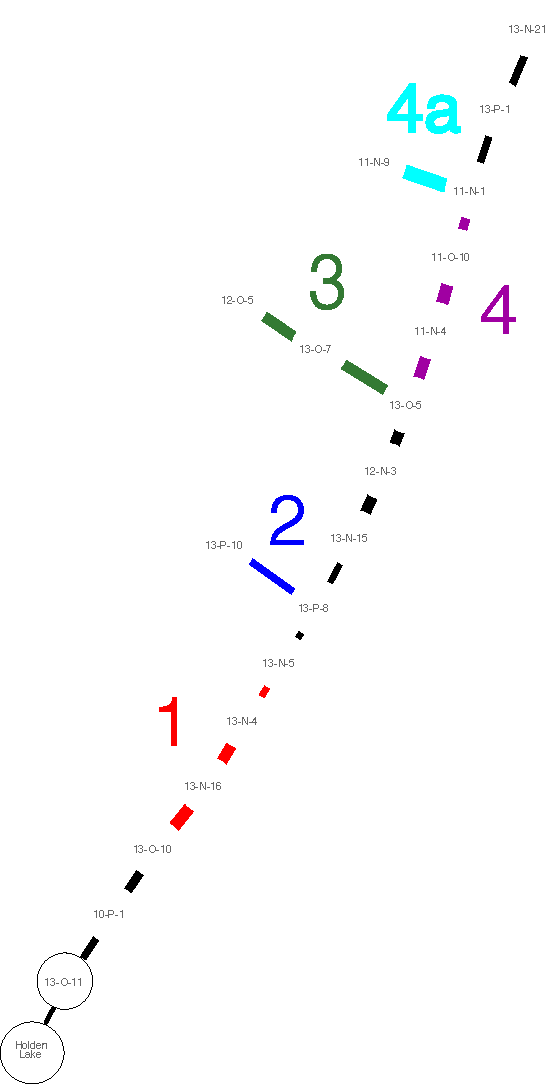
\includegraphics[scale=0.5]{graphics/multipleseriation/pfg-minmax-network-both-solutions.pdf}
\caption{Seriation solution with frequency and continuity seriation for PFG \citeyearpar{Phillips1951} ceramic assemblages in 
the Lower Mississippi River Valley, as analyzed by Lipo \citeyearpar{Lipo2001a} and re-analyzed by \citet{lipomadsendunnell2015}.  There are no differences between frequency and continuity ordering algorithms in analyzing this set of assemblages, and thus only one graph is shown.}
\label{img:pfg-both-solutions}
\end{figure}

To that end, we extended the Lower Mississippi River Valley example
from our recent work \citep{lipomadsendunnell2015} by comparing
frequency and continuity seriation algorithms on the same set of
assemblages.  The result is
depicted in Figure \ref{img:pfg-both-solutions}. The result is identical
-- the two solutions are isomorphic.  

We are archiving seriation data sets, with supporting information including geography 
if available, and licenses (if available
and required) in an open-source repository on Github:  \url{https://github.com/mmadsen/seriation-datasets}.  Over time we expect to be able to employ the data sets to create automated
test suites for new seriation algorithms and software implementations.  We are also adding scripts
which execute our IDSS software for any of its implemented algorithms, for the data sets.  We welcome 
contributions to the data repository (please contact Madsen for more details).  

Empirical data sets suitable for determining comparable the two seriation algorithms might be are hard to come by,
and typical cases have a small number of assemblages, which tend to yield small linear seriations without complex 
structure.  Thus, we also employ a Monte Carlo or simulation approach to sampling many possible seriations, 
performing both frequency and continuity on sampled data, and comparing the structure of the resulting seriations.
We employed the \emph{SeriationCT} simulation framework described in detail in Chapter \ref{chap:computational-metapopulation}
to generate samples of simulated cultural transmission, with time averaging, on realistic metapopulation-style models
of regional interaction.  The simulations were performed for purposes of examining whether seriations can be 
diagnostic of the evolving social networks within which cultural transmission occurred in the past.  For purposes
of the present study, however, the simulation results presented an opportunity to compare ordering algorithms.

Because the ``lineage splitting'' transmission scenario (described in Chapter \ref{chap:computational-metapopulation}, in Section 
\ref{metapop:sec:transmission-scenarios}) yielded seriation graphs with detailed branching structures, it presented a more 
conservative comparison than the complete networks, which had a much higher incidence of straight linear orderings.  Thus,
we randomly sampled 50 simulated data sets from the lineage splitting model, and performed seriations with our IDSS software, using both frequency (unimodality) and continuity (distance minimization) settings.




Seriation of artifact assemblages is inherently a regional-scale
problem, whether for chronology or tracking interaction and social
learning processes. Thus, the fundamental abstraction for modeling is a
graph or network which (a) represents the intensity of contact,
migration, and interaction between communities of people at any given
point in time, (b) allows the set of communities to evolve, with some
communities going away and others originating over time, and (c)
representing how both the pattern and intensity of inter-community
contacts evolves over time. Social network or graph models, especially
weighted graphs, form an essential ingredient for this type of modeling,
but need to be extended to the temporal dimension.

We measure whether frequency and
continuity solutions are identical by testing whether the solution
graphs are isomorphic, which means that the same vertices are connected
to the same neighbors by the same edges. Of the 50 simulation runs
examined here, in 80\% of cases the continuity and frequency seriations
give an exactly identical solution. Of the remaining non-identical
solutions, we find that the differences nearly always involve the
repositioning of a single assemblage. In the next section, we examine
such a case in detail to understand what drives such differences when
they occur.

\subsection{Examining a Solution Which
Differs}\label{examining-a-solution-which-differs}

\begin{figure}[ht]
\centering
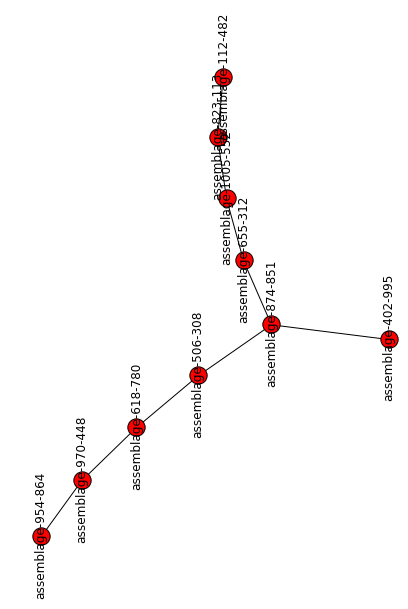
\includegraphics[scale=0.4]{graphics/multipleseriation/f8a6f378-freq.png}
\caption{Frequency seriation solution for simulation run f8a6f378 on the "lineage splitting" regional interaction model.}
\label{img:differing-freq}
\end{figure}

Of the differing solutions, we selected one (f8a6f378) at random to show
the details of how frequency and continuity solutions differ. Figures
\ref{img:differing-freq} and \ref{img:differing-cont} depict the
frequency and continuity seriations, respectively, in the form of graphs
which connect assemblages which are ``adjacent'' in the seriation
solution. This makes it easier to see where an assemblage is really part
of several solutions, which can indicate lineage splitting or
differentiation occurring over space. We introduced this format for
seriation solutions in our recent article on IDSS seriation
\citep{lipomadsendunnell2015}.

\begin{figure}[ht]
\centering
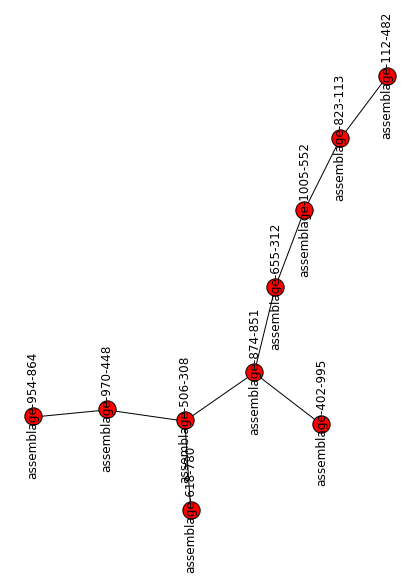
\includegraphics[scale=0.4]{graphics/multipleseriation/f8a6f378-cont.png}
\caption{Continuity seriation solution for simulation run f8a6f378 on the "lineage splitting" regional interaction model.}
\label{img:differing-cont}
\end{figure}

Although the graphs are laid out slightly differently (as a function of
an automated graph layout algorithm), it is apparent that most of the
seriation ordering is the same. Simulated assemblage 954-864 anchors one
end of the ordering, while assemblage 112-482 anchors the
other.\footnote{Simulated assemblage names here reflect geographic
  coordinates, since regional interaction models often bias interaction
  and migration by location or neighborhood.} Both solutions also show a
branch for assemblage 402-995, which belongs to one of the two lineages
after the connections between two sets of communities is lost. It is a
single assemblage branch because of the vagaries of sampling assemblages
out of the total set of communities in this example. The main difference
between the solutions comes in assemblage 618-780 and where it connects.
In the frequency solution it occurs ``inline'' while in the continuity
solution, interassemblage distance is minimized by removing it to a
small branch of its own.

\begin{sidewaystable}[p!]
\centering
\begin{tabular}{@{}llllllllll@{}}
\toprule
Assemblage Name & 6022-0-1767 & 36526 & 36557 & 7005-0-1767 & 7628-0-1767 & 0-9222-3 & 1-0-1767 & 3771 & 6996-4-3 \\ \midrule
assemblage-954-864  & 10                & 160   & 0     & 49                & 92                & 0           & 0           & 0     & 9         \\
assemblage-970-448  & 0                 & 155   & 0     & 74                & 128               & 0           & 0           & 0     & 14        \\
assemblage-618-780  & 123               & 50    & 0     & 164               & 121               & 0           & 13          & 0     & 14        \\
assemblage-506-308  & 107               & 58    & 0     & 199               & 114               & 0           & 9           & 0     & 13        \\
assemblage-874-851  & 81                & 66    & 0     & 165               & 0                 & 0           & 162         & 6     & 17        \\
                    &                   &       &       &                   &                   &             &             &       &           \\
assemblage-874-851  & 81                & 66    & 0     & 165               & 0                 & 0           & 162         & 6     & 17        \\
assemblage-655-312  & 0                 & 52    & 16    & 111               & 0                 & 20          & 269         & 6     & 26        \\
assemblage-1005-552 & 0                 & 53    & 32    & 72                & 0                 & 61          & 182         & 41    & 8         \\
assemblage-823-113  & 0                 & 145   & 81    & 0                 & 0                 & 64          & 132         & 10    & 14        \\
assemblage-112-482  & 0                 & 24    & 151   & 0                 & 0                 & 157         & 81          & 49    & 9         \\
                    &                   &       &       &                   &                   &             &             &       &           \\
assemblage-874-851  & 81                & 66    & 0     & 165               & 0                 & 0           & 162         & 6     & 17        \\
assemblage-402-995  & 106               & 65    & 0     & 29                & 0                 & 0           & 192         & 0     & 7         \\ \bottomrule
\end{tabular}
\caption{Raw data for frequency seriation for simulation run f8a6f378, grouped into blocks corresponding to the branches of the solution graph}
\label{f8a6f378-freq-table}
\end{sidewaystable}

Viewed in traditional tabular view of the type counts in Tables
\ref{f8a6f378-freq-table} and \ref{f8a6f378-cont-table} or as
traditional centered bar charts in Figures \ref{img:frequency} and
\ref{img:continuity}, several features are apparent. First, there are
apparent violations of unimodality in the frequency seriation. But given
our IDSS algorithm, we calculate a 95\% confidence interval around each
type count given the total sample size, and thus there are small
differences (compared to the larger values) which are not statistically
significant. Second, we can see that continuity solutions allow
violations of unimodality (e.g., assemblage 823-113) but come up with
the same overall structure. To us, this shows that unimodality is
sufficient but not necessary for using a seriation method to track the
spatiotemporal structure of cultural transmission.

\begin{sidewaystable}[p!]
\centering
\begin{tabular}{@{}llllllllll@{}}
\toprule
Assemblage Name & 6022-0-1767 & 36526 & 36557 & 7005-0-1767 & 7628-0-1767 & 0-9222-3 & 1-0-1767 & 3771 & 6996-4-3 \\ \midrule
assemblage-954-864 & 10 & 160 & 0 & 49 & 92 & 0 & 0 & 0 & 9 \\
assemblage-970-448 & 0 & 155 & 0 & 74 & 128 & 0 & 0 & 0 & 14 \\
assemblage-506-308 & 107 & 58 & 0 & 199 & 114 & 0 & 9 & 0 & 13 \\
assemblage-874-851 & 81 & 66 & 0 & 165 & 0 & 0 & 162 & 6 & 17 \\
assemblage-655-312 & 0 & 52 & 16 & 111 & 0 & 20 & 269 & 6 & 26 \\
assemblage-1005-552 & 0 & 53 & 32 & 72 & 0 & 61 & 182 & 41 & 8 \\
assemblage-823-113 & 0 & 145 & 81 & 0 & 0 & 64 & 132 & 10 & 14 \\
assemblage-112-482 & 0 & 24 & 151 & 0 & 0 & 157 & 81 & 49 & 9 \\
 &  &  &  &  &  &  &  &  &  \\
assemblage-874-851 & 81 & 66 & 0 & 165 & 0 & 0 & 162 & 6 & 17 \\
assemblage-402-995 & 106 & 65 & 0 & 29 & 0 & 0 & 192 & 0 & 7 \\
 &  &  &  &  &  &  &  &  &  \\
assemblage-506-308 & 107 & 58 & 0 & 199 & 114 & 0 & 9 & 0 & 13 \\
assemblage-618-780 & 123 & 50 & 0 & 164 & 121 & 0 & 13 & 0 & 14 \\ \bottomrule
\end{tabular}
\caption{Raw data for continuity seriation for simulation run f8a6f378, grouped into blocks corresponding to the branches of the solution graph}
\label{f8a6f378-cont-table}
\end{sidewaystable}

\begin{figure}[ht]
\centering
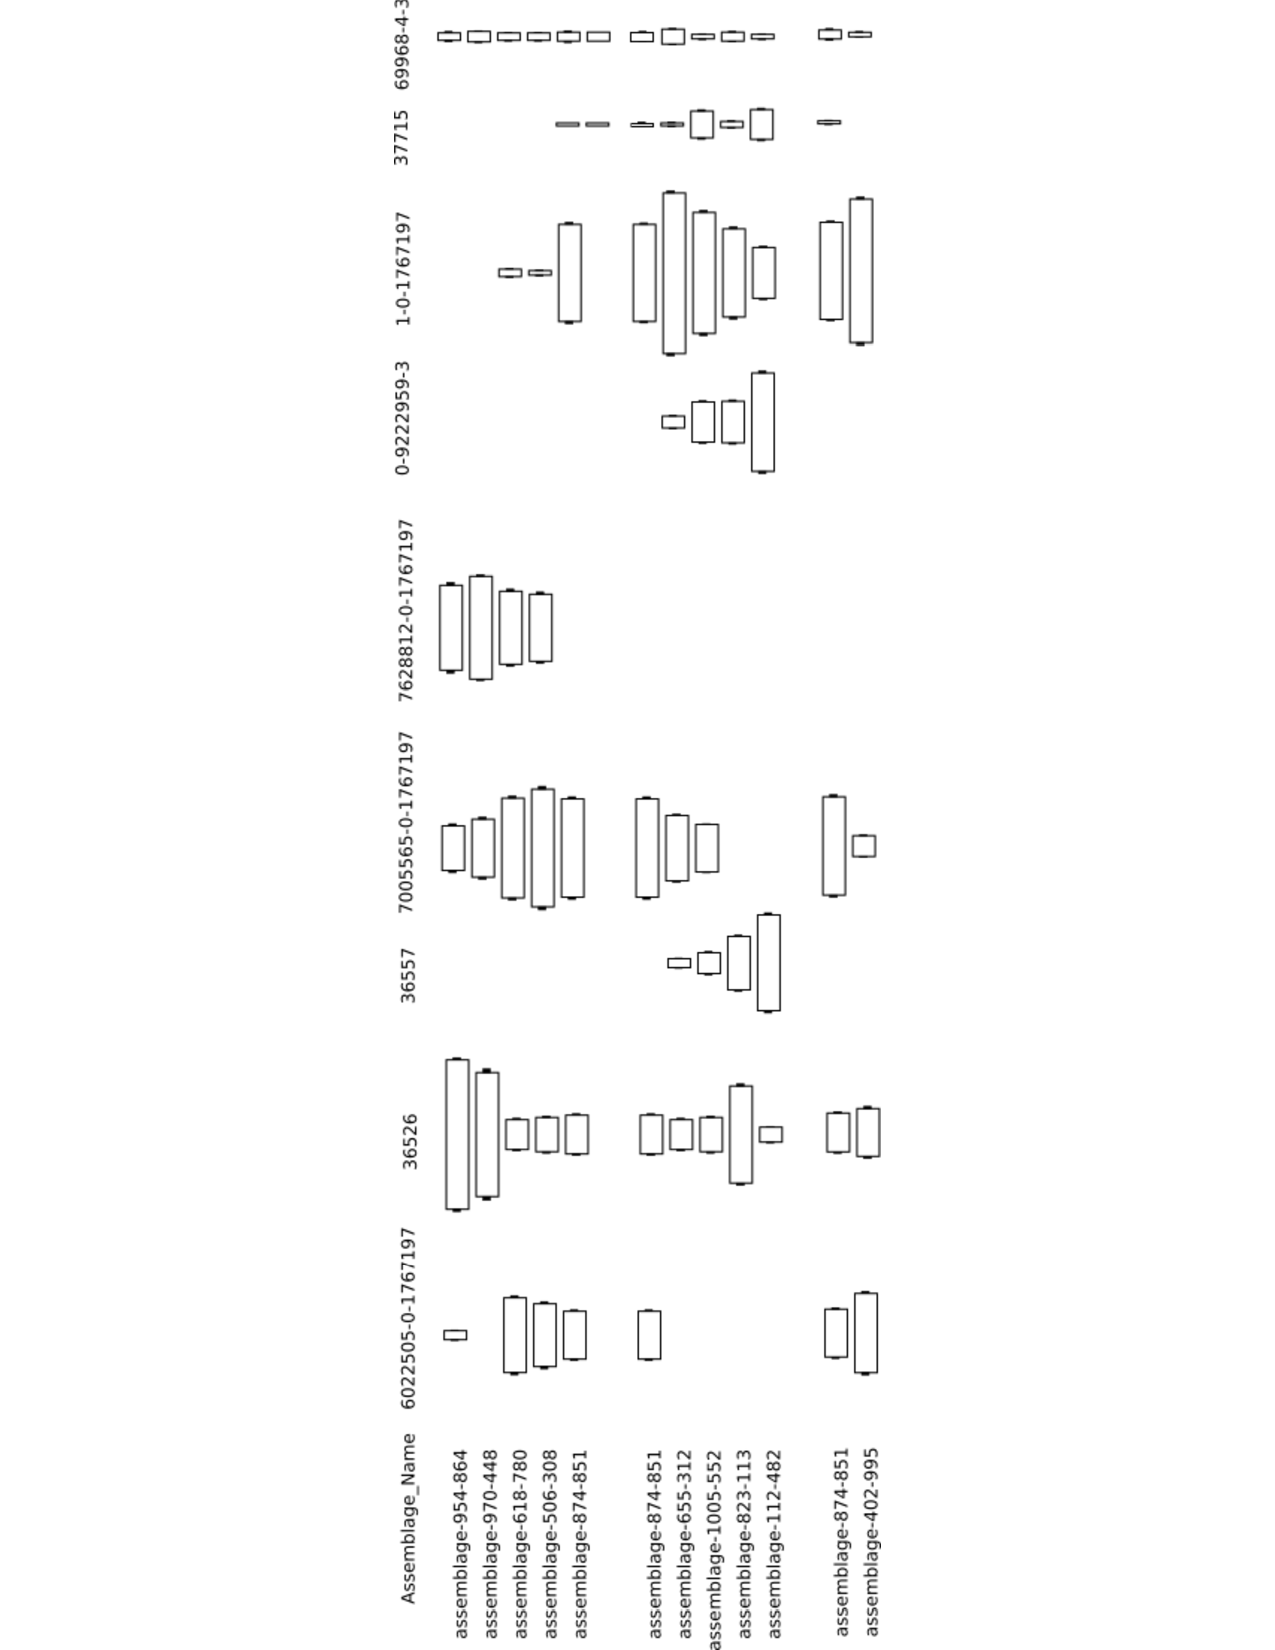
\includegraphics[scale=0.5]{graphics/multipleseriation/frequency.pdf}
\caption{Centered bar chart representation of the relative frequencies of type for simulation run f8a6f378 built with the IDSS frequency seriation algorithm. The groups correspond to the branches of the solution graph.}
\label{img:frequency}
\end{figure}

\begin{figure}[ht]
\centering
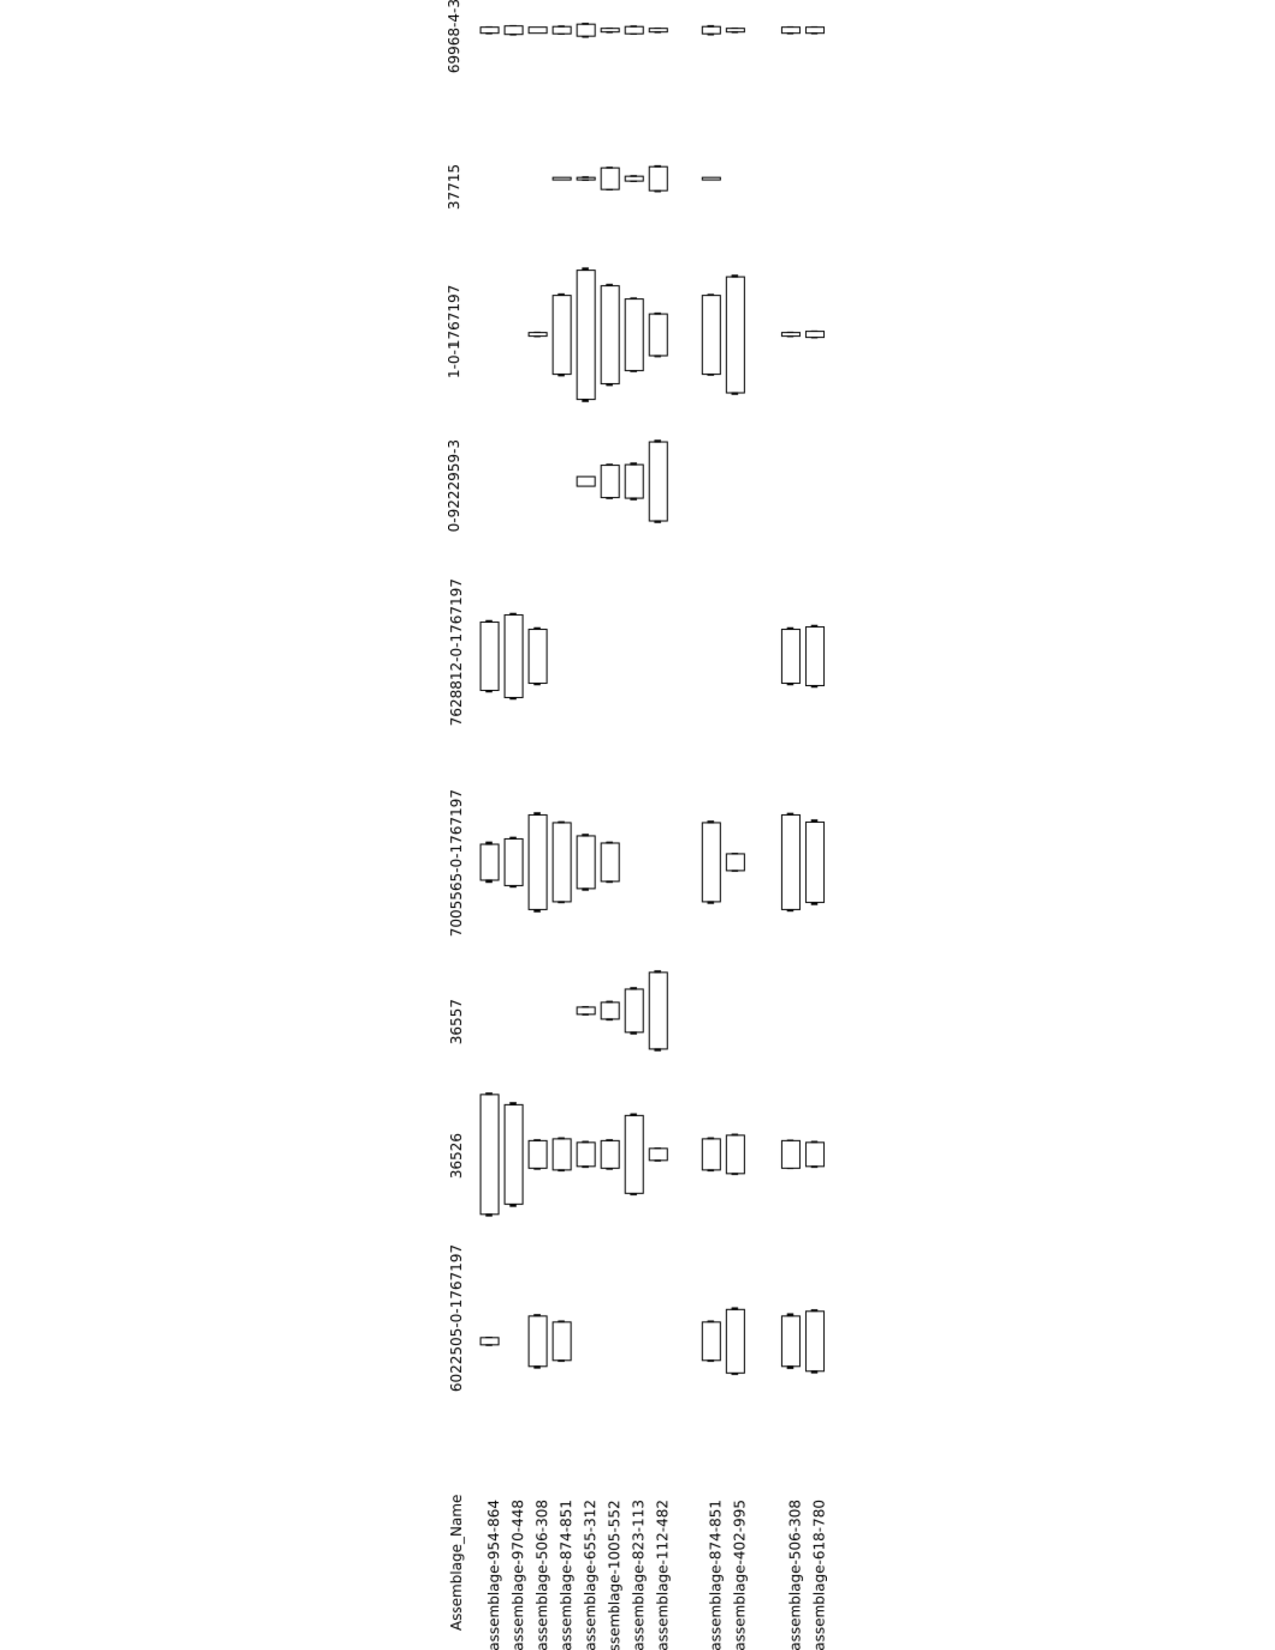
\includegraphics[scale=0.5]{graphics/multipleseriation/continuity.pdf}
\caption{Centered bar chart representation of the relative frequencies of type for simulation run f8a6f378 built with the IDSS continuity seriation algorithm. The groups correspond to the branches of the solution graph.}
\label{img:continuity}
\end{figure}


\section{Discussion}\label{discussion}

The fact that distance minimization can function as a seriation ordering
algorithm is not a new idea. Not only has there been development of the
idea within archaeological circles in the work of Kadane, Shepherdson,
and others, but distance minimization of one type or another underpins
most classical multivariate statistics and nearly all of contemporary
machine learning. Our principal contributions here have been to
explicate the relationship between different seriation ordering
algorithms, and to reintroduce distance minimization in an ``exact''
rather than statistical form.

Exact distance minimization as a means of tracing patterns of cultural
transmission is only possible if we do not coerce the data into a single
linear ordering, as has been the practice in all previous work. In these
previous applications, the departures from linearity have been
considered statistical noise or ``stress,'' and disregarded. From a
culture transmission model, however, noise only enters the seriation
problem as sampling error of counts or frequencies given the size of
sample taken by the analyst. We can control this type of noise by using
bootstrap confidence intervals around the empirical frequencies when we
make ordering decisions. Our IDSS software system does so by default.
Thus, once the effects of sampling are controlled departures from
linearity cannot be noise, but are telling us something else about our
data. In our judgment, those departures from perfect linearity are
telling us about the simultaneous effects of spatial variation, temporal
order, and the structure of the social networks of interaction within
which past cultural transmission occurred.

Thus, our approach to both frequency and continuity seriation allows
partial solutions (each of which \textbf{is} a valid linear ordering) to
agglomerate to form graphs or networks of solutions, given vertices
(assemblages) which overlap between the sub-solutions. The resulting
seriation graphs give us a more complete picture of the multiple causes
that drive seriations than do traditional linear orders, whether perfect
or coerced by a statistical method.

The search for additional ordering methods led us to reconsider distance
minimization methods, and although it is not unexpected that such
methods work, it is a happy result. Continuity techniques have a much
lower computational burden than searching for unimodality, especially as
the number of assemblages gets large. For the Phillips, Ford and Griffin
assemblages discussed here, the frequency solution took 25.2 seconds on
an 8 core system, while continuity analysis took 0.955 seconds, for a
speedup of 26x. This performance difference should be taken as a minimum
on the difference between algorithms, because our current algorithm for
unimodality analysis is parallelized for a critical section across all
of those cores, while continuity is still a serial algorithm and only
uses a single core. Realistically, we should see a much larger speedup
with further development, especially given the wealth of parallel
algorithms for distance metric computations in contemporary machine
learning. The latter will allow continuity methods to be fruitfully used
even for ``big'' datasets of the type easily gathered in online
settings. This method effectively has no limit as to the number of
assemblages that can be analyzed.

Seriation is among the oldest of the purely archaeological methods for
determining both chronology and cultural relatedness, but we find that
it continues to repay detailed exploration by archaeologists and
students of cultural evolution. It is fully complementary to
phylogenetic methods and cladistics in many ways, especially in its
ability to use detailed information about trait abundances and the
spatial pattern of those abundances instead of largely presence/absence
data on character states. This makes seriation, in our view, the method
of choice for ``mesoscale'' problems and questions.



    
    \chapter{Behavioral Modernity and the Cultural Transmission of Structured Information:  The Semantic Axelrod Model}
    \label{chap:semanticaxelrod-paper}
    
\begin{description}[leftmargin=-1\labelwidth]
\item[\textsc{Abstract}] Cultural transmission models are coming to the fore in explaining increases in the Paleolithic toolkit richness and diversity. During the later Paleolithic, technologies increase not only in terms of diversity but also in their complexity and interdependence. As \citet{mesoudi2008learning} have shown, selection broadly favors social learning of information that is hierarchical and structured.  We believe that teaching provides the necessary scaffolding for transmission of more complex cultural traits.  Here, we introduce an extension of the Axelrod \citeyearpar{axelrod1997} model of cultural differentiation in which traits have prerequisite relationships, and where social learning is dependent upon the ordering of those prerequisites. We examine the resulting structure of cultural repertoires as learning environments range from largely unstructured imitation, to structured teaching of necessary prerequisites, and we find that in combination with individual learning and innovation, high probabilities of teaching prerequisites leads to richer cultural repertoires.  Our results point to ways in which we can build more comprehensive explanations of the archaeological record of the Paleolithic as well as other cases of technological change..

\item[\textsc{Source}]  Published in \textit{Learning Strategies and Cultural Evolution During The Paleolithic}, edited by Alex Mesoudi and Kenichi Aoki, 2015, in the series \textit{Replacement of Neanderthals By Modern Humans}, Springer.  Co-authored with Carl P. Lipo.
\end{description}

%%%%%%%%%%%%%%%%%%%%%%%%%%%%%%%%%%%%%%%%%%%%%%%%%%%%%%%%%%%%%%%%%%%%%%%%%%%%%%%%%%%%%%%%%




\section{Introduction}\label{semax:sec:introduction}

Although humans and our hominid ancestors have been cultural animals
throughout our evolutionary history, an important change occurred in our
lineage during the Middle and Upper Paleolithic. For millennia our
ancestors manufactured relatively small toolkits and their material
culture was remarkably similar across continental distances and over
many generations. Beginning in the Middle Paleolithic and continuing
through the Upper Paleolithic, the archaeological record reflects an
explosion in our cultural repertoire. Over tens of thousands of years,
artifactual toolkits shift from sets of relatively few objects with
multiple uses to large collections of functionally-specialized tools
that, employed increasingly complex technologies and that were
manufactured from an enriched range of materials. The changes in
artifacts suggest that human solutions to the problems of everyday life
became regionalized and differentiated. Further, the economic basis of
our lives began to broaden and also, in many areas, to become
specialized \citep{bar2002upper, d2011evolution, guy2005mosaic}.

While early researchers believed that the Upper Paleolithic resulted
from a singular ``revolution'' in human evolution leading to
behaviorally modern homo sapiens, this view is held by a minority of
paleoanthropologists and archaeologists today
\citep[e.g.,][]{klein2009human}. Careful examination of the Middle
Paleolithic archaeological record especially in Africa and the Near East
suggests that this change in behavior did not occur as a single distinct
event, instead occurring over a long period of time since much of the
enriched material culture we later characterize as the ``Upper
Paleolithic'' had precursors. In addition, this change now appears to be
patchy and fitful, with modern features appearing and frequently being
lost again
\citep{bouzouggar200782, d2007additional, d2011evolution, guy2005mosaic, mcbrearty2000revolution, mcbrearty2007down}.
Nor does behavioral modernity map neatly to biological taxa and their
movements, given that evidence for the precursors of fully modern
behavior is abundant in deposits associated with Neaderthals in addition
to modern \emph{Homo sapiens} \citep{Villa:2014kl}.

The ``learning hypothesis'' studied in this series of volumes makes the
plausible claim that behavioral modernity is the product of cumulative
changes in the way cultural information was acquired and retained across
generations \citep{Nishiaki2013Introduction}, thus providing a potential
explanation for the slow evolution of ``modern'' features, its
patchiness in space and time, and the lack of a neat mapping between
hominin taxonomy and material culture. In short, according to the
learning hypothesis, behavioral modernity arose through a change or
changes in the way social learning operated within hominin groups, with
those groups adopting richer modes of cultural learning surviving and
spreading compared to those who retained simpler forms of social
learning.

Within the umbrella of the learning hypothesis, there are many ways in
which social learning and thus intergenerational cultural transmission
could have changed, and an increasing amount of research is focused upon
formulating and testing different models. One class of studies is
focused upon factors exogeneous to the learning or imitation process
itself. Shennan
\citetext{\citeyear{shennan2000population}; \citeyear{shennan2001demography}}
proposed that population size has a powerful effect on diversity within
cultural transmission processes, which Henrich showed in the case of
toolkit element loss during a Tasmanian population bottleneck
\citep{henrich2004}. In a similar line of reasoning, Kuhn
\citeyearpar{Kuhn2013Cultural-Transm} argues that low population size
and density put Neanderthals in a situation where innovations spread
slowly and ultimately led to their demise relative to modern humans.
Furthermore, a growing set of experimental studies clearly show a
relationship between accumulation of complex cultural traits and the
number of cultural ``models'' from whom individuals can learn
\citep{muthukrishna2014sociality, derex2013experimental, kempe2014experimental}.
Not all studies have shown a strong association between population size
and cultural diversity, however. Collard and colleagues, find little
association in a linked series of comparative studies
\citep{collard2011drives, collard2013population, collard2013risk, collard2013plos}.
Finally, in his analysis of the overall evolutionary rate, Aoki
\citeyearpar{Aoki2013Determinants-of} found that innovation rates were
more important than population size to determining the rate of evolution
in a population.

To us, this body of work indicates that while population size is an
important parameter in mathematical models, it may be better understood
as a second-order effect in the real world, interacting with a myriad of
other factors and thus often dominated by those factors. Another
important factor is the structure of bands or demes into larger regional
metapopulations. Network topology, for example, is known to have a
substantial effect upon contagion or diffusion processes
\citep[e.g.,][]{castellano2009statistical, smilkov2012influence}. Thus,
it is likely that regional structure has critical effects on the
outcomes we can expect from a single social ``learning rule.'' Along
these lines, Premo \citeyearpar{premo2012local} has examined whether
metapopulation dynamics that include local extinction and recolonization
might provide an improved account for the retention and expansion of
diversity.

A second group of studies has focused upon endogeneous changes to social
learning processes. Many authors in this volume series, for example,
have looked at aspects of the way individuals learn skills and acquire
information \citep{Aoki2013Determinants-of, Nishiaki2013Introduction}.
We know that learning and teaching styles vary across human groups, and
formal modeling efforts are beginning to make clear that such variation
has evolutionary consequences that might lead to a rapid expansion of
the human cultural repertoire \citep{Nakahashi2013Cultural-Evolut}.
Those populations which increased the amount or effectiveness of
teaching would have a fitness advantage over those who relied upon
imitation and ``natural pedagogy'' in passing along technological and
foraging knowledge
\citep{Csibra:2011dx, Fogarty:2011gv, Terashima2013}.
Demography and population structure would then play an important role in
reinforcing the fitness differences which different learning strategies
would create, as pointed out by Kuhn
\citeyearpar{Kuhn2013Cultural-Transm}.

Ultimately, a full ``learning explanation'' for behavioral modernity
will be multifacted, including demographic and spatial changes as well
as changes to the mechanisms of social learning and technological
innovation themselves. Sterelny \citeyearpar[p.61]{sterelny2012evolved}
sums up this kind of multifactorial approach to behavioral modernity
well:

\begin{quote}
\ldots{}the cultural learning characteristic of the Upper Paleolithic
transition and later periods of human culture---social transmission with
both a large bandwidth and sufficient accuracy for incremental
improvement---requires individual cognitive adaptations for cultural
learning, highly structured learning environments, and population
structures that both buffer existing resources effectively and support
enough specialization to generate a supply of innovation.
\end{quote}

In research designed to explore how the structure of a learning
environment affects the results of social learning, Creanza and
colleagues \citeyearpar{Creanza2013Exploring-Cultu}, Aoki
\citeyearpar{Aoki2013Determinants-of}, Nakahashi
\citeyearpar{Nakahashi2013Cultural-Evolut}, and Castro and colleagues
\citeyearpar{Castro201474} developed models that examine how explicit
teaching (as opposed to simple imitation) affects the overall
evolutionary rate or cultural diversity in a population. Castro et al.,
for example, find that cumulative cultural transmission requires active
teaching in order to achieve fidelity across generations. Our work in
this chapter follows these authors, focusing on the nature of
transmitted information itself and the effects of teaching upon the
richness of structured technological knowledge.

In particular, we suggest that when knowledge is structured such that
skills and information must be learned in sequences, high fidelity
learning environments are critical to evolving ever-richer cultural
repertoires, of the type seen in behaviorally modern assemblages. To
formalize this idea, we construct a model which:

\begin{itemize}
\itemsep1pt\parskip0pt\parsep0pt
\item
  Represents cultural traits as hierarchically structured, in order to
  study increases in complexity,
\item
  Has a learning rule sensitive to the order in which cultural traits
  are acquired, with multiple levels of fidelity, and
\item
  Has a mechanism (such as homophily) that allows cultural
  differentiation endogeneous to the model.
\end{itemize}

As we alter the ``learning environment'' in our models from less to more
frequent teaching of traits and their prerequisites, we expect to see
greater diversity, larger structured sets of traits persisting in the
population, and greater differentiation of the population into
``different'' cultural configurations. We also expect that individual
innovation, independent of the social learning context, will play a role
in the accumulation of cultural complexity by allowing a population to
explore increasingly large spaces of technological design possibilities;
this expectation is concordant with Aoki's
\citeyearpar{Aoki2013Determinants-of} result in Volume I of this series.

In this chapter, we introduce a simulation model which combines a
hierarchical trait space capable of expressing dependencies or semantic
relationships between skills and information \citep{mesoudi2008learning}, and a
modified version of Robert Axelrod's \citeyearpar{axelrod1997}
homophilic social learning model which allows us to examine the
conditions under which evolution in a hierarchical design space leads to
cultural differentiation. After describing the model, we study its
dynamics and provide an initial assessment of its suitability for
studying the onset of behavioral modernity in the later Paleolithic.
Models like this begin to move beyond diffusion dynamics, bringing the
actual meaning and relations of traits into the modeling process. Hence,
we call these ``semantic Axelrod'' models, and believe that such models
form a platform for formalizing the type of multi-factor hypotheses
necessary to examine major transitions in human evolution, such as
``behavioral modernity.''

\section{The Semantic Axelrod Model for Trait
Prerequisites}\label{semax:sec:the-semantic-axelrod-model-for-trait-prerequisites}

Much of our technical knowledge, whether of stone tool manufacture,
throwing clay pots, or computer repair, is built from simple tasks, bits
of background knowledge, and step-by-step procedures
\citep{neff1992ceramics, Schiffer1987}. These pieces of cultural
information are not simply a set of alternative options, which can be
mixed and matched in any combination. Instead, there are dependencies
and relationships between items which affect how skills and information
are learned and passed on between individuals. Some items will be
related in time, as steps in a process. Others will be related by
subsumption: arrowheads are a subclass of bifacial stone tools, and
require many of the same production techniques as bifaces used in other
projectiles. Still others will be related as sets of alternatives:
choices of surface treatment for a given ceramic paste, given the firing
regime selected, for example. To date, most archaeological models of
tool production have focused upon temporal relations in the construction
of an artifact, as in ``sequence models'' or
``$\textrm{cha\^ine op\'eratoire}$,'' but it is important to remember
that other representations are possible, including trees and more
general graphs to capture relations of use, reworking, or discard
\citep{Bamforth:2008kq, Bleed:2008in, Ferguson:2008ce, Hogberg:2008fj, bleed2001trees, bleed2002obviously, Schiffer1987, stout2002skill}.

Given conscious reflection, we describe and organize our knowledge and
skills in many ways, but it is common (especially while learning a new
skill) to think of a complex process as a ``script'' or ``recipe''
\citep{schank1977scripts}. Experts in a task or field may not represent
their knowledge this way, having internalized such structures below the
conscious level. Experts will often know more than one way to accomplish
any given goal, and be able to repurpose and recombine methods and
tools, as opposed to the simpler, more linear or tree-based recipes of
the novice or student
\citep[e.g.,][]{Bleed:2008in, bleed2002obviously, stout2002skill}.
Nevertheless, it is common to teach or learn new information and skills
in a stepwise manner.

In this chapter, we focus not on the execution steps of a recipe (and
thus not on sequence models), but the relations between skills and
information \emph{during the learning process}. In specific, we focus
upon the \emph{prerequisite} relationships that exist between cultural
traits, since the ordered dependencies between skills and information
form one of the structures within social learning occurs during
development (and into adulthood). Some pieces of information or skills
must be in place before a person can effectively learn or practice
others. Examples from our own childhoods abound: one needed to
understand addition and subtraction and multiplication before learning
long division; in order to make soup, we need to understand how to
simmer rather than boil, how to chop and slice, what ingredients might
be combined, and so on. The fact that knowledge and skills build upon
one another make prerequisite relations between cultural traits
ubiquitous. In this chapter, we represent prerequisite relations as
trees in the graph-theoretic sense \citep{diestel2010graph}, replacing
the ``nominal scale'' structure of ``locus/allele'' models or
paradigmatic classifications and some typologies \citep{Dunnell1971},
but we emphasize that the tree models we discuss here are still
classifications and thus analytic tools, designed to allow us to measure
variation in the archaeological record, not reconstruct emic models of
Paleolithic technologies.

Our model also requires a way of representing a changing learning
environment, in ways that create higher fidelity and greater possibility
for building cumulative knowledge. In real learning environments, there
are many possibilities, but deliberate teaching and apprentice learning
are repeatedly seen across human groups as ways that naive individuals
can reliably learn the complex skills and information needed for
foraging, artifact production and maintenance, and navigating an
increasingly rich social world. The point of structuring the learning
environment with teaching and/or apprenticeship is to give the learner
skilled models to imitate, shortcut trial and error when acquiring a
skill, provide a reference for needed information, and to guide
individuals to put their information and skills together into
appropriate sequences to accomplish an overall goal. Apprenticeship and
formalized teaching provide a social learning ``scaffold,'' helping to
lower the amount of individual trial and error learning needed to master
a body of material \citep{wimsatt2007reproducing, wimsatt2007re}.

Within a standard discrete-time simulation model of a social learning
process, we can model this type of learning environment with the
following modifications:

\begin{enumerate}
\def\labelenumi{\arabic{enumi}.}
\itemsep1pt\parskip0pt\parsep0pt
\item
  Represent the order in which skills and information need to be
  acquired as a series of trees, with vertices representing traits
  (either a skill or piece of information), and edges the prerequisite
  relations between them.
\item
  Disallowing individuals the ability to copy traits from a cultural
  model for which they do not have necessary background or
  prerequisites, given the relations in the applicable tree model.
\item
  Creating a probability that individuals, if disallowed a trait, can be
  taught one of the needed prerequisites instead by that cultural model,
  leading to the potential accumulation of fuller knowledge and skills
  over time.
\end{enumerate}

By changing the probability that individuals learn a missing
prerequisite trait, we can ``tune'' the learning environment. Low
probabilities might correspond, for example, to a learning environment
where individuals can observe others executing a production step, but
are given little or no instruction or guidance on what they need to know
in order to successfully master it. High probabilities of learning
prerequisites would correspond, on the other hand, to environments where
individuals receive instruction, or work together with a more skilled
individual who guides them toward learning the information and skills
they lack. In the next section, we discuss our model of trait
relationships and the learning environment in more detail.

\subsection{Representation of Traits And Their
Prerequisites}\label{semxax:sec:representation-of-traits-and-their-prerequisites}

In order to represent the ``prerequisite'' relations between a number of
cultural traits, we organize the traits into trees\footnote{A tree is a
  graph with no cycles or loops. That is, a tree is a connected graph on
  $n$ vertices that possesses at most $n-1$ edges
  \citep{diestel2010graph}. Furthermore, in this chapter we are
  concerned with \emph{rooted} trees, in which one vertex is
  distinguished as the ``origin'' of the tree, giving rise to a
  hierarchical structure.}, where nodes higher in the tree represent
knowledge, skills, or concepts which are necessary for traits further
down the tree. Let us consider the different skills and information
necessary for the construction of a single artifact, say a dart thrown
by an atlatl. An artisan will possess information about different raw
materials, an understanding of what materials are suitable for specific
purposes, skills and information concerning the knapping of different
types of bifaces, methods of hafting bifaces into different kinds of
shafts, and so on. Stout \citeyearpar{stout2011stone} organized such
knowledge into ``action hierarchies,'' which represent sequences of
actions, sets of choices, and optional elements for the construction of
a class of stone tools, drawing the representation from Moore's
\citeyearpar{moore2010grammars} graphical notation.

\begin{figure}[h] 
\centering 
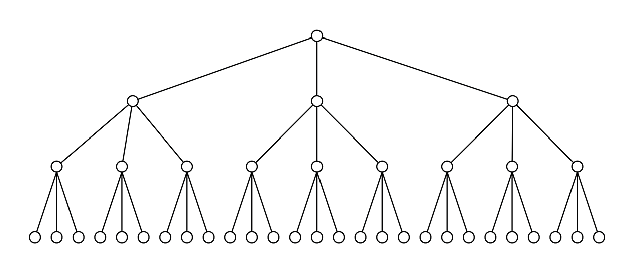
\includegraphics[]{graphics/semanticaxelrod/balanced-trait-tree-3-3.eps} 
\caption{A single trait tree, represented by a balanced tree with branching factor 3 and depth factor 3, order 40.  In our model, nodes higher in the tree represent prerequisites for nodes lower down the tree.  Each instance of the model will have several or many of these trees in the design space.} 
\label{semax:img:trait-tree} 
\end{figure}

We should emphasize that employing tree structures to represent learning
dependencies is a modeling choice. Other choices may be sensible as
well. General graphs could represent webs of relations between concepts
or skills, and multigraphs (replacing adjacency matrices with tensors)
can represent different types of relations in a single structure
\citep{ICML2011Nickel_438}. For purposes of the present chapter, we are
interested in the order in which people usually \emph{learn} skills and
information, rather than the order in which steps are executed. The
difference is potentially significant, in that two adjacent steps in a
sequence might involve very different information, tools, or skills,
which can be learned in parallel without dependencies. Because, in our
model, traits cannot be learned unless an individual possesses the
necessary prerequisites, we introduce the idea of a ``learning
hierarchy,'' which is a division of Stout's action hierarchy into
components which are learned with ordered dependencies, and independent
components represented in separate trees. For example, one might learn
about the sources of good lithic raw materials, independent of learning
how to perform different percussion techniques. In our model, each of
these independent areas is represented by a separate tree of traits.

\begin{figure}[h] 
\centering 
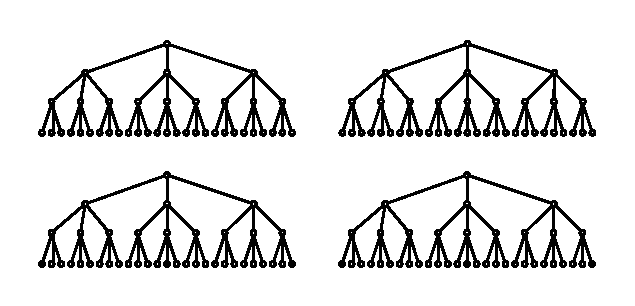
\includegraphics[scale=0.6]{graphics/semanticaxelrod/design-space-4-trees.eps} 
\caption{A design space composed of 4 independent trees, each tree with branching factor 3 and depth factor 3, order 40.  We also studied larger design spaces with 16 independent trees, and with larger branching and depth factors.} 
\label{semax:img:design-space-4} 
\end{figure}

In each simulation model, we begin with a trait or ``design space'' that
incorporates several independent sets of traits \citep{o2010cultural}.
The overall design space of a simulation model is thus a
forest\footnote{A forest is a graph composed of multiple components,
  each of which is a tree.}, composed of several trees (Figure
\ref{semax:img:design-space-4}). For each tree in a learning hierarchy, we
employ balanced trees which have the same number of nodes at each level,
to provide a simplified model of a design space with which to begin our
exploration of this class of social learning model, although real design
spaces are undoubtedly more complex in their geometry. Each tree in our
model is specified by a branching factor $r$ and depth $h$. As a result,
each trait tree in the design space has $\sum_{i=0}^{h} r^i$ traits.

The tree depicted in Figure \ref{semax:img:trait-tree} thus has 40 vertices,
for example. In this chapter, we examine both small (4 trees) and larger
(16 trees) design spaces, to see how learning may differ in problems
involving design spaces of different size and complexity. We examine
trees with combinations of branching and depth factors of 3 and 5. Thus,
a design space with 4 trees with branching and depth factors of 3 (as in
Figure \ref{semax:img:trait-tree}) would have 160 traits, whereas a design
space with 16 trees of branching and depth factors of 5 would have a
total of 62,496 traits.\footnote{We initially chose 6 as the limit on
  branching and depth factors, but found that we cannot calculate
  certain symmetry statistics, such as the size of the automorphism
  group, on trees that large using existing tools. Even a tree with
  $r=5, h=6$ has over $10^{1623}$ possible symmetries, and an attempt to
  calculate the symmetries for $r=6, h=6$ did not complete given the
  memory limits of the computers we had available.} Even the small
design spaces we consider here create a large space for cultural change
and differentiation, given the number of possible trees one can
construct on even 40 vertices.\footnote{If we consider each trait to be
  unique and non-interchangeable, the number of unique trees with unique
  vertex labels is $n^{n-2}$ by Cayley's theorem
  \citep{diestel2010graph}. For example, for each trait tree of 40
  vertices, there are roughly $10^{60}$ possible trees. Even if we
  consider traits to be interchangeable (e.g., we look at the abstract
  topology of trees rather than the details of individual traits), there
  are \emph{at least} $10^{16}$ possible unlabelled rooted trees on 40
  vertices (using Otter's \citeyearpar{otter1948number} approximation).}
In the experiments reported here, the overall size of the design space
remains constant over time, which is a simplifying assumption as we
develop this class of structured information models. In future work, we
will explore the role of invention in episodically creating large new
regions of design space for the evolving population to explore.

Given the total ``design space'' represented by a forest of trait trees,
each individual in our model is initialized with a small number of
``initial'' traits. Initial traits are chosen randomly but heavily
weighted towards the roots of the trees to represent the fact that our
knowledge starts out basic and sparse. In general, all of the design
spaces modeled here are larger than populations will explore within the
bounds of a simulation run. In the next sections we describe the social
learning model, modified from Robert Axelrod's original, by which each
simulated population evolves within this tree-structured design space,
and will return to the specifics of how an initial culture repertoire is
chosen.

\subsection{The Axelrod Model of Social Learning and
Differentiation}\label{semax:sec:the-axelrod-model-of-social-learning-and-differentiation}

Robert Axelrod \citeyearpar{axelrod1997} formulated a model aimed at
studying the conditions under which simple learning rules could lead to
cultural differentiation, rather than a single fixed state (which is the
result of simpler neutral or diffusion models). This makes it useful as
a starting point for understanding phenomena such as behavioral
modernity, in our view. Axelrod's model combines social learning, in the
form of random copying, a spatial structure to interaction, in the form
of localized copying of neighbors on a lattice, and the tendency to
interact most strongly with those to whom we are already culturally
similar (homophily). The model displays a rich and interesting set of
behaviors, and has been extensively studied by social scientists and
physicists \citep{castellano2009statistical}. First we review the basic
model, and in the following section our modified algorithm.

\subsubsection{Axelrod's Original Model}\label{semax:sec:axelrods-original-model}

The original model locates $N$ individuals on the nodes of a regular
lattice or grid, but various network structures have also been studied.
Each individual is endowed with $F$ integer variables
$(\sigma_1,\ldots,\sigma_F)$, that can each assume $q$ values. In the
original model, each variable is a ``cultural feature'' each of which
can assume $q$ ``traits.'' In each step, a randomly chosen individual
$i$ and a random neighbor $j$ are selected, and ``interact'' with
probability equal to the overlap between their cultural repertoire.
Overlap, in the basic model, is simply the fraction of features for
which $i$ and $j$ possess the same trait value:

\begin{equation}\label{semax:eq:axelrod}p(i,j) = \frac{1}{F} \sum_{f=1}^{F} \delta_{\sigma_f(i)\sigma_f(j)}\end{equation}

where $\delta_{i,j}$ is Kronecker's delta function, taking the value $1$
when its two arguments are equal and $0$ otherwise. When individuals
interact, the focal individual $i$ takes the trait value of its neighbor
for one of the features where the two individuals differ.

Interaction has no effect when two individuals already possess identical
cultural repertoires, and there is no probability of interaction if
individuals have no traits in common. This eventually causes the model
to reach an absorbing state where no further changes are possible.
Instances of the model are initialized with a random distribution of
traits among individuals, and left to update until the steady state is
reached. The evolution of the population leads to two classes of
absorbing states: (a) a ``monocultural'' state in which all individuals
share the same set of variables, and (b) a ``polycultural'' state in
which subpopulations exist which share the same set of variables within
the group, and are completely different from their neighbors.

Which of the two results is reached, and the statistical character of
``polycultural'' states when they exist, depends mainly upon the number
of traits possible $q$ for each cultural feature. For small values of
$q$, individuals share many traits with their neighbors, interactions
are thus frequent, and one domain comprising a single set of traits will
grow to become fixed within the entire population. In contrast, when the
value of $q$ is high, individuals start out sharing very few traits,
with interactions that are correspondingly less frequent. Regions of
uniform cultural variation do grow, but as they do, sets of individuals
who share no traits at all (and thus do not interaction) grow as well,
and often prevent any single regional culture from expanding to fix
within the population.

Many variants of the basic Axelrod model have been studied, including
the addition of ``drift'' via the introduction of copying error,
situating agents on different types of complex networks, the addition of
an external ``field'' to simulate the effects of mass media, and copying
that obeys a ``conformist'' or majoritarian rule by selecting the most
common trait among the neighbor set
\citep{castellano2000nonequilibrium, de2009effects, flache2006sustains, GonzalezAvella:2007p6910, GonzalezAvella:2007p6912, gonzalez2005nonequilibrium, gonzalez2006local, Klemm:2003p7031, Klemm:2003p7112, Klemm:2005tb, Lanchier:2010p16999, Lanchier:2012ur}.
In general, modifications of the basic model can reduce the tendency of
the model to produce polycultural solutions, or change the time scale or
location of the critical point.

\subsubsection{Semantic Extensions to the Axelrod
Model}\label{semxax:sec:semantic-extensions-to-the-axelrod-model}

We begin each simulation with $N$ (100, 225, or 400) agents, arranged on
a square grid. A design space is created, with some number of trait
trees (4 or 16), with uniform branching factors and depth factors (3 or
5). An example of such a tree is shown in panel A of Figure
\ref{semax:img:prereq}. Initial traits (and their prerequisites) are chosen
randomly across the configured number of trait trees, as follows. For
each individual, we select a random number $t$ between 1 and 4, and
repeat the trait selection process $t$ times for that individual. In
each selection, we choose a random tree in the design space, and then
select a depth in the tree for the trait, given by
$d  \sim \textrm{Poisson}(0.5)$. This biases trait selection towards the
root of the tree, as one would expect in young or inexperienced
individuals. We then walk $d$ steps into the tree, making uniform random
selections for the children of each vertex. The path of vertices thus
constructed is added to the individual's trait set, giving them an
initial trait and its necessary prerequisites. One such initial trait is
shown in Panel B of Figure \ref{semax:img:prereq}. Given that individuals
begin with a small number of initial traits (between 1 and 4, selected
randomly), and their prerequisites, the initial trait endowment of an
individual is between 1 and $4h$, where $h$ is the maximum depth of the
design space (either 3 or 5 in the experiments reported here).\footnote{At
  maximum, this yields some individuals who begin the simulation with up
  to 20 traits. The median number of traits in samples taken after 6-10
  million time steps is considerably higher--259 traits per cultural
  configuration or region. Thus, cultural repertoires in the simulation
  grow through copying and innovation, as expected.}

\begin{figure}[htbp] 
\centering 
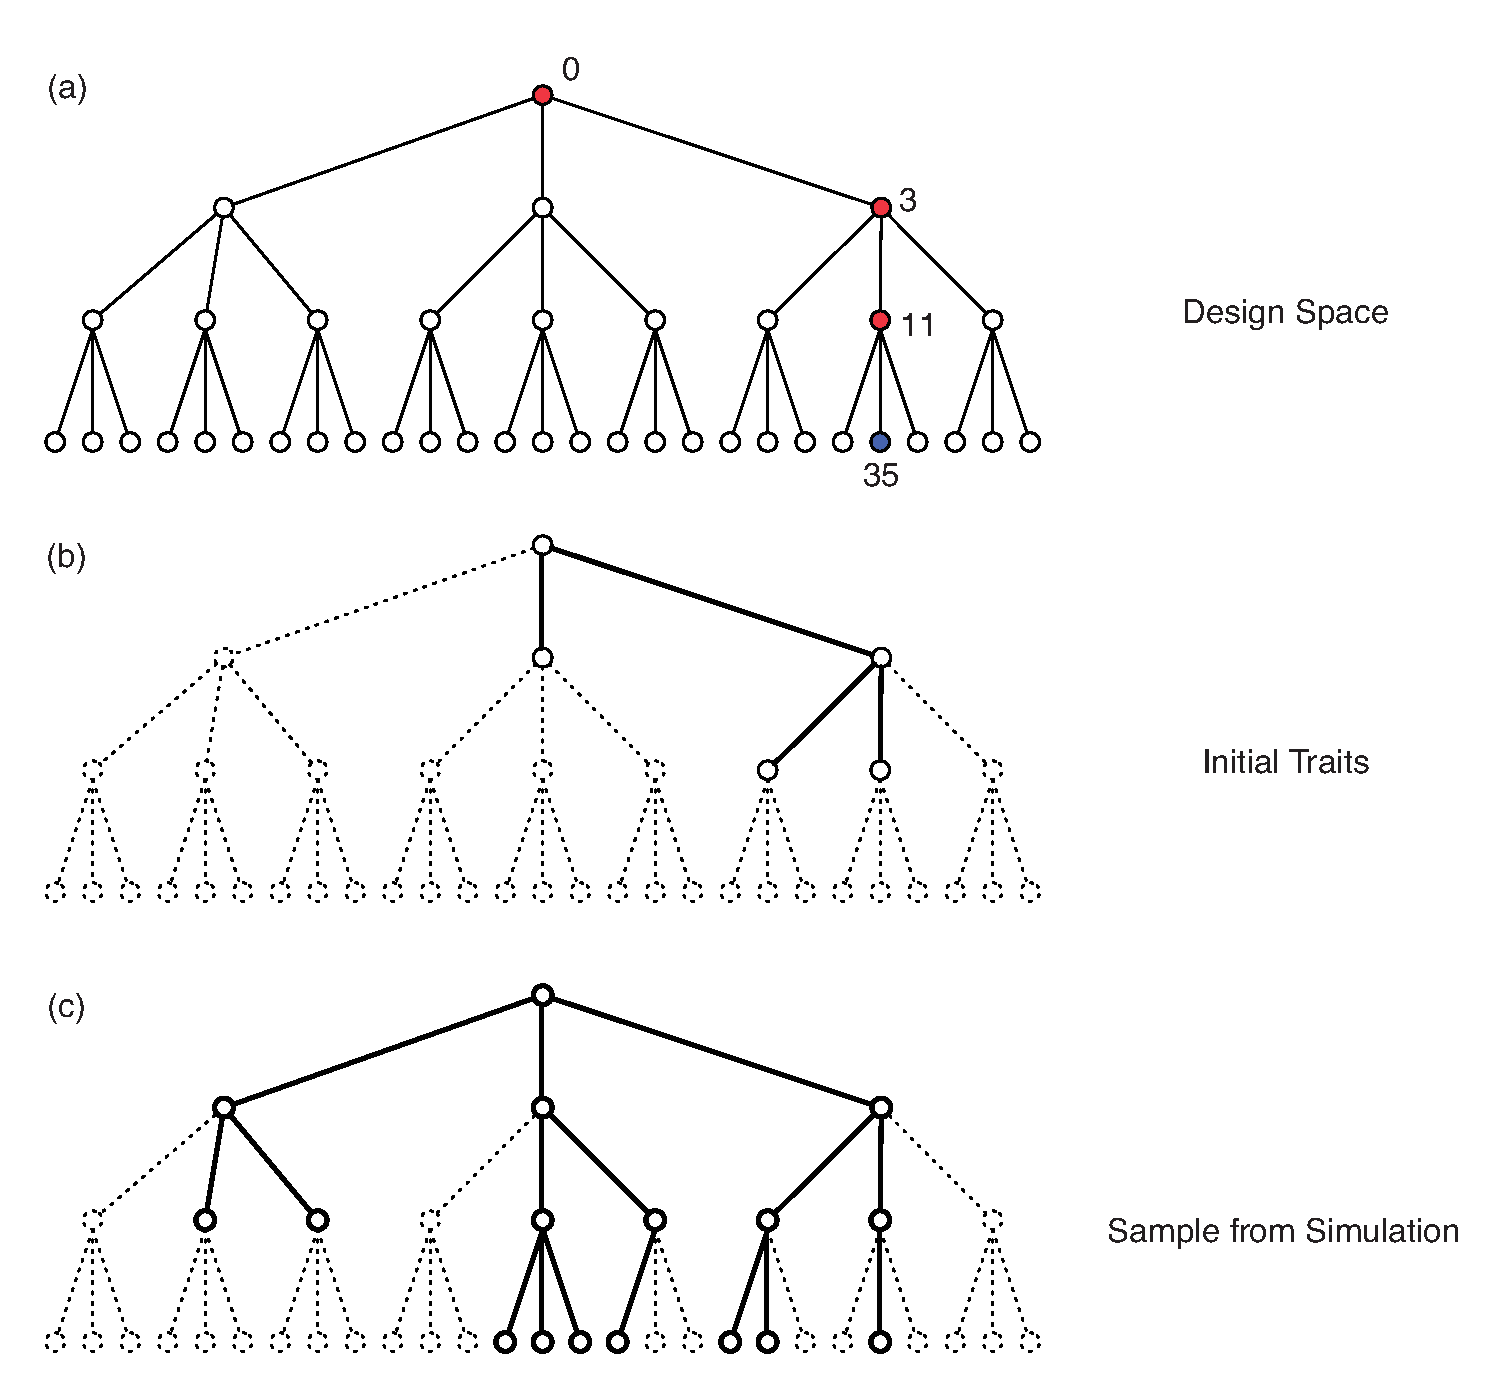
\includegraphics[scale=0.5]{graphics/semanticaxelrod/design-init-final.eps} 
\caption{Illustration of a design space composed of a single trait tree, along with a random initial trait chosen from the design space, and a final sample from a simulation run, showing the evolution of traits within the design space.  Also shown in the top panel are the ``prerequisites'' for a cultural trait (35), as an example.} 
\label{semax:img:prereq} 
\end{figure}

Once the population is initialized, the simulation runs a discrete
approximation to a continuous-time model. In other words, only one agent
changes at each elemental time step, as in the original Axelrod model
and the Moran model of population genetics and its cultural version
\citep{aoki2011rates, moran1962statistical, moran1958random}. At each
step, an agent (A) is chosen at random, and a random neighbor of A is
then selected (agent B). Their probability of interaction is given by
the overlap of trait sets, which is most simply calculated as the
Jaccard overlap between the set of tree vertices each possesses, thus
replacing Equation \ref{semax:eq:axelrod} with:

\begin{equation}J(A,B) = \frac{|V(A) \cap V(B)|}{|V(A) \cup V(B)|}\end{equation}

where $V(i)$ represents the vertex list for trait trees held by
individual $i$ in the population.

If the agents end up interacting, agent A observes the traits currently
possessed by B, and selects a trait (T) that it does not already possess
to learn. If agent A has the necessary prerequisite traits for the
selected trait, it can learn trait T. If not, there is a probability
$\mathbb{P}(l)$ that B can teach A a necessary prerequisite for T
instead. This simulates the process of agent B structuring the learning
environment of A through formal instruction or apprenticeship, for
example. If such a prerequisite learning event occurs given
$\mathbb{P}(l)$, agent A learns the most fundamental of T's
prerequisites that it does not already possess. For example, agent A
might require the trait closest to T (e.g., trait 11 in Figure
\ref{semax:img:prereq}, if the original trait targeted was 35).

Additionally, at each time step, there is a probability $\mathbb{P}(m)$
that one random individual in the population will learn a new trait (and
necessary prerequisites) that it does not already possess. For example,
if an innovation event occurs and an agent discovers trait 35 by
individual trial and error learning, we assume that the agent also
discovered traits 0, 3, and 11. Thus innovation can introduce one trait
to the population, or a linked set depending upon its prerequisites and
what the innovating individual already ``knows.'' This model of
innovation simulates an ongoing process of individual learning
unconnected to social learning or teaching within the population.
Because this functions much like ``infinite-alleles mutation'' in the
classical Wright-Fisher neutral models \citep{Ewens2004}, or like noise
terms in Axelrod, Ising, or Potts models
\citep{castellano2009statistical}, we will refer to this as the ``global
innovation rate'' in this chapter.

One of the editors noted that this model of innovation may not be as
realistic as an alternative, where random innovations would be
``discoverable'' only with the correct prerequisites in place. We
believe that innovation in the face of skill or knowledge prerequisites
is continuous between these two models. Occasionally one will discover a
new piece of knowledge or develop a skill, having learned surrounding
and related knowledge. In other situations, individuals may learn
sequences and sets of information or skills by trial and error and
``tinkering.'' The ``size'' of innovations that can be learned purely by
individual trial and error should thus vary between these extremes,
biased towards the ``small'' end of the range. Our selection of an
innovation model where individuals discover a trait and its
prerequisites thus potentially overestimates the effect of individual
learning, but it made certain graph operations easier, and can be
relaxed in future models.

Each simulation run lasts $10^7$ steps, which yields between $10^4$ and
$10^5$ copying events per individual, depending upon population
size.\footnote{100,000 was chosen as a compromise for running large
  batches of simulations in parallel. Some simulation runs, especially
  in small design spaces with very high prerequisite learning rates, can
  converge to a monocultural solution and quasi-stable equilibrium quite
  quickly; in the largest design spaces and low learning rates,
  convergence may never occur even though the process is well-mixed.
  However, the processes have reached a quasi-stable equilibrium,
  verified by examining samples at different times for secular trends in
  median and mean values, which were not found.} Since we do not
explicitly model the interaction between cultural transmission and
biological reproduction here, we can interpret the model as representing
either fine-grained learning within individuals over the course of their
lifetimes, or long-term cultural evolution within a fixed size
population where we are not modeling fitness. We felt this
simplification was appropriate in a pilot study exploring structured
information models, but a more detailed study would include dynamics on
two time scales: developmental learning and evolutionary dynamics given
birth and death. Samples are taken beginning at 6 million steps, and
sampling at an interval of 1 million steps, and record the trait trees
seen in the population. An example of such a sampled tree is shown in
Panel C of Figure \ref{semax:img:prereq}. For reference, the full algorithm
for each copying step is given in the Appendix as Algorithm
\ref{semax:alg:tree-prereq-axelrod}.
\section{Measuring Cultural Diversity and the Results of Structured
Learning}\label{semax:sec:measuring-cultural-diversity-and-the-results-of-structured-learning}

Each sample from a simulation run is composed of the distinct sets of
trait trees possessed by individuals in the population, along with
summary statistics. If a simulation run converges to a monocultural
solution, the sample will have one set of trait trees, which are shared
across the entire population. In other cases, there will be clusters of
cultural configurations which might be unique to a single individual, or
shared by some number of agents. Each cluster will be composed of some
number of trait trees (typically, the number configured for the
simulation run: 4 or 16, but perhaps a subset), and each trait tree will
be the result of many agents learning traits and their prerequisites
socially, and for runs with a non-zero mutation rate, by individual
learning or innovation. Each cluster will thus have some number of
traits, typically higher (often much higher) than the initial endowment
given to the population.

\begin{figure}[htbp] 
\centering 
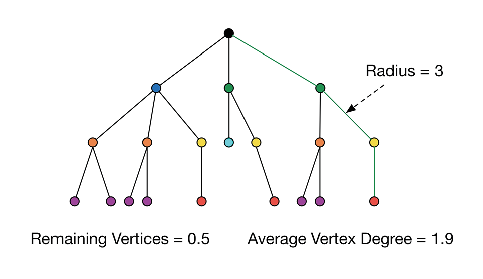
\includegraphics[]{graphics/semanticaxelrod/equil-trait-tree.eps} 
\caption{An example set of traits at the conclusion of a simulation run, extracted from a simulation with branching factor 3 and depth factor 3, and a single trait tree as the trait space.  The remaining density of vertices, mean vertex degree, and radius of the tree are noted.  Vertex colors denote ``structural equivalence'' classes or ``orbit structure,'' as measured by adjacency patterns, and is one measure of the symmetries present in the tree.} 
\label{semax:img:final-tree} 
\end{figure}

From the sampled trait trees, we calculate summary statistics as
follows. The ratio of the number of traits in the sample to the full
design space size (or ``remaining density'' of traits) is one measure of
trait richness. The radius of a rooted tree is the number of edges in
the path from root to the furthest edge. The average radius of trees in
a sample (or its ratio to the depth of the design space) is another
richness measure, aimed at measuring whether knowledge with multiple
prerequisites is being learned within the simulated population.
Similarly, in the original design space, the branching factor describes
how many children each node in the tree started with, so measuring the
average vertex degree gives us a rough measure of how broad a cultural
repertoire is. Each of these measures is illustrated in Figure
\ref{semax:img:final-tree} for an example tree selected from our data.

In addition to these simple numerical measures comparing final trees to
the original design space, it is useful to measure something about the
overall ``shape'' of the trees themselves. One way of formalizing this
notion is to examine the \emph{symmetries} of the final trait trees.
Examining Figure \ref{semax:img:final-tree}, if we ignore the exact identities
of traits for the moment, it is apparent that there are repeating
patterns. For example, the left-most branches each terminate in a pair
of leaves. This pattern is repated on the second right-most branch.
These types of repeating patterns are computationally expensive to
search for in large sets of trees, but we can summarize them by
considering trait trees as algebraic objects and examining their
\emph{automorphisms}.

An automorphism is a function which maps an object to itself, in such a
way that the structure of the object is preserved
\citep{rotman1995introduction}. Graph automorphisms map vertices in a
graph to each other, preserving properties such as the adjacency pattern
of edges. The six vertices which mark the repeating pattern of
leaf-pairs in Figure \ref{semax:img:final-tree} are an automorphism of the
tree, and thus are symmetries we can measure. An overall measure of
``how symmetrical'' (or ``how many interchangeable patterns'') there are
in a graph possesses given by the total number of automorphisms found,
called the size of the automorphism group or $|\textit{Aut}(G)|$
\citep{godsil2001algebraic}. A tree with no repeating patterns will thus
have an automorphism group size of 1, indicating that the only symmetry
is the entire tree itself. A balanced tree with branching and depth
factors of 3, as depicted in Figure \ref{semax:img:trait-tree}, has
approximately $1.3 \times 10^{10}$ automorphisms. The more repeating
patterns there are in trait trees, the more automorphisms they will
possess.

Because group sizes grow quickly and the accuracy of performing
calculations with truly astronomical numbers is low, another possible
measure of the symmetries present is to count the \emph{classes} of
equivalences into which vertices fall. The \emph{orbits} of the
automorphism group are the sets of vertices which are interchangable by
some permutation that preserves structure. For example, the graph in
Figure \ref{semax:img:trait-tree} has five orbits, with each vertex at a given
level interchangable (in a structural sense). Similarly, the six leaf
vertices that are part of pairs in Figure \ref{semax:img:final-tree} are part
of the same orbit; in this illustration, each orbit is given a different
color to highlight their equivalence. For each cultural region found
when sampling a simulation, we calculate the size of the automorphism
group and the number and multiplicity (frequency) of orbits. For this
analysis, we employ the \emph{nauty + Traces} software by Brendan McKay
and Adolfo Piperno \citep{McKay201494}.\footnote{Nauty+Traces can be
  downloaded at \url{http://pallini.di.uniroma1.it/}. We employed
  version 2.5r7 for this research.}

\section{Experiments}\label{semax:sec:experiments}

Given a modified Axelrod model on a tree-structured trait space, we
expect to see greater cultural diversity, differentiation among groups
of individuals, and larger sets of traits as the ``learning
environment'' is tuned from a low to high probability of teaching and
learning among individuals. We also expect that individual innovation,
independent of the social learning context, will increase the amount of
the technological design space that a population explores, which leads
to enhanced opportunities for differentiation even through simple random
copying. Here we measure cultural differentiation by the number of
clusters of individuals who share the same trait trees when we sample
the population.

Second, we looked at whether highly structured learning environments,
represented here by higher probabilities of naive individuals gaining
the prerequisites for the skills and information they encounter with
peers, led to deeper and richer cultural repertoires. We explore a
number of ways of measure the richness of a cultural repertoire in a
model with structured relations between traits, through the use of graph
properties and symmetry measures. The measures used are those described
above: the tree radius (or depth), mean vertex degree, the fraction of
remaining vertices, and the size of the automorphism group of sampled
trait forests. Finally, we began to examine how the structured learning
environment might interact with demography, by simulating the same
parameters across two sizes of population.

For this chapter, we examined populations of size 100, 225 and 400, to
begin to examine the effects of population size. For these populations,
we examined design spaces that were small (4 trait trees) and large (16
trait trees). Within each size, we further examined combinations of
branching factor and depth factor with values of 3 and 5, thus yielding
8 total sizes of design space (Table
\ref{semax:tab:axelrod-design-space-size}).

\begin{table}[H]
\begin{tabular}{|c|c|c|c|}
\hline
\textbf{Branching Factor} & \textbf{Depth Factor} & \textbf{Number of Trait Trees} & \textbf{Size of Design Space}\\ 
\hline
3 & 3 & 4 & 160\\ 
\hline 
5 & 3 & 4 & 624\\ 
\hline 
3 & 5 & 4 & 1456\\ 
\hline 
5 & 5 & 4 & 15624\\ 
\hline 
3 & 3 & 16 & 640\\ 
\hline 
5 & 3 & 16 & 2496\\ 
\hline 
3 & 5 & 16 & 5824\\ 
\hline 
5 & 5 & 16 & 62496\\ 
\hline 
\hline
\end{tabular}
\caption{Size of design space for different trait tree configurations}
\label{semax:tab:axelrod-design-space-size}
\end{table}

Further, we examined three levels of global mutation or innovation rate:
zero, or no mutation, and 0.00005 and 0.0001. Such rates created a
constant supply of new innovations, but several orders of magnitude less
frequent than copying and prerequisite learning events. The full set of
parameters are given in Table \ref{semax:tab:axelrodct-sim-parameters}. In
this pilot study, for each combination of all of the above parameters,
we performed 25 replications. With 5 samples per simulation run, this
yielded 10,963,691 samples of cultural regions.

\begin{table}[H]
\begin{tabular}{|p{0.6\textwidth}|p{0.4\textwidth}|}
\hline
\textbf{Simulation Parameter} & \textbf{Value or Values} \\ 
\hline
Population rate at which new traits arise by individual learning & 0.0, 5e-05, 0.0001\\ 
 \hline 
Maximum number of initial traits (not including their prerequisites) each individual is endowed with & 4\\ 
 \hline 
Number of distinct trees of traits and prerequisites & 4, 16\\ 
 \hline 
Population sizes & 100, 225, 400\\ 
 \hline 
Replicate simulation runs at each parameter combination & 25\\ 
 \hline 
Maximum time after which a simulation is sampled and terminated & 10000000\\ 
 \hline 
Individual probability for being taught a missing prerequisite & 0.05, 0.1, 0.2, 0.3, 0.4, 0.5, 0.6, 0.7, 0.8, 0.9\\ 
 \hline 
Number of branches at each level of a trait tree & 3, 5\\ 
 \hline 
Depth of traits in each trait tree & 3, 5\\ 
 \hline 
\hline
\end{tabular}
\caption{Parameter space for simulations described in this chapter}
\label{semax:tab:axelrodct-sim-parameters}
\end{table}

\section{Results}\label{results}

We begin by noting that compared to the original Axelrod model, or
neutral and biased copying models, the dynamics of our semantic Axelrod
model are highly variable. A very wide range of outcomes is possible for
each parameter combination, especially when the size of the design space
is large. Some variables, such as the average vertex degree of sampled
trait trees, are strongly overlapping across all learning rates and do
not appear diagnostic of different learning environments, at least in
these initial experiments. Given the large amount of variability in the
dynamics, larger numbers of replications would be useful, although this
is computationally quite expensive at present.\footnote{The simulations
  reported here ran on a cluster of 6 compute-optimized ``extra large''
  Linux instances on Amazon's EC2 computing cloud, for a total of 17
  days of wall clock time and 2075 CPU hours. We plan further
  optimizations to the simulation code to make larger samples
  economically feasible.} That said, several features of the data are
strongly suggestive that hierarchical trait models have potential in
modeling cumulative technological evolution, making the computational
expense worthwhile.

\subsection{Cultural Diversity}\label{semax:sec:cultural-diversity}

\begin{figure}[htbp]
    \centering
    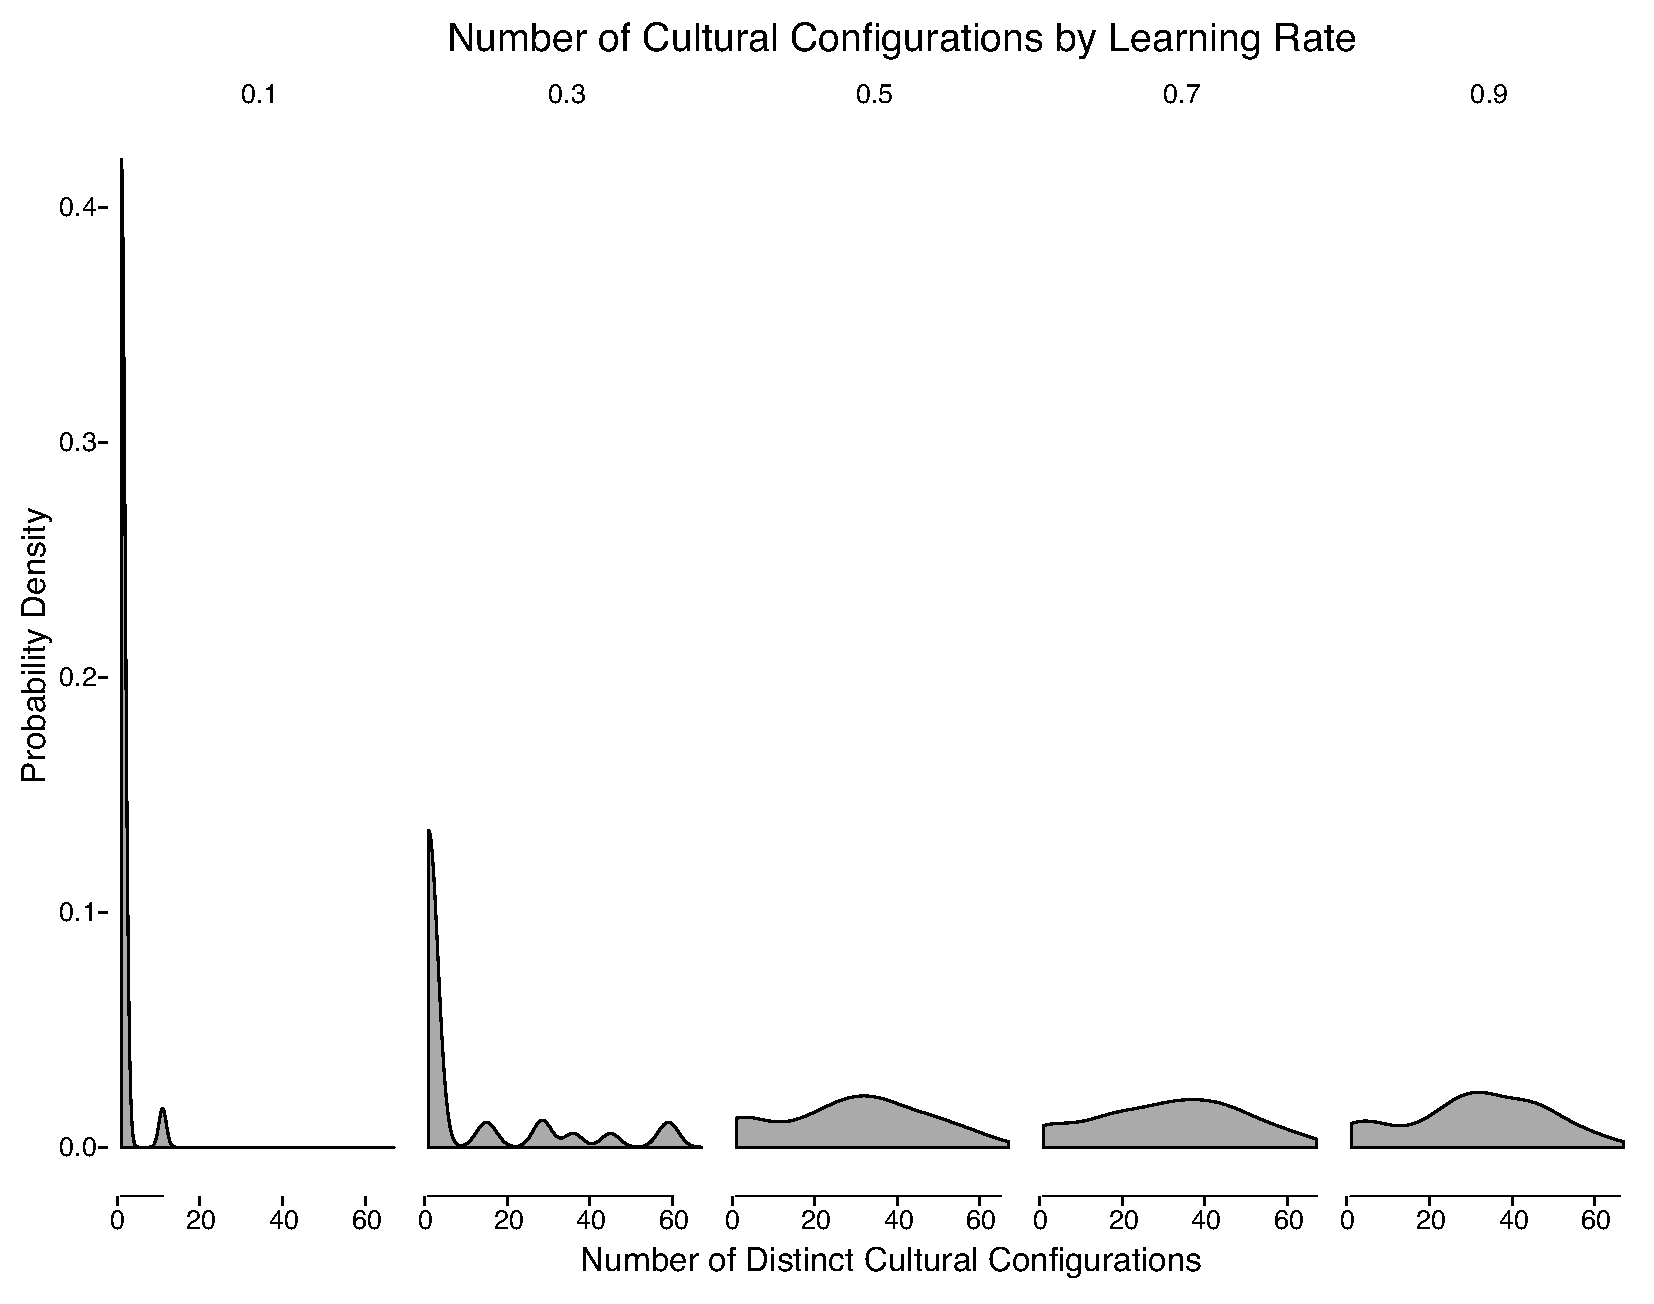
\includegraphics[scale=0.4]{graphics/semanticaxelrod/small-trait-high-innovation-num-configs.eps}
    \caption{Number of cultural configurations in simulations with the smallest trait space (160 total traits in 4 trees), and a high individual innovation rate ($10^{-4}$).}
    \label{semax:img:culture-count-sm-trait-high-innov}
\end{figure}

Variation among individuals is foundational to evolutionary processes,
and is the raw material from which differentiation between regions and
cultural groups is constructed. Figure
\ref{semax:img:culture-count-sm-trait-high-innov} depicts the number of
cultural configurations (i.e., trait trees) in a population of size 100,
for the smallest trait space with only 160 total traits, and relatively
high levels of individual innovation. For example, in the left-most
panel the large peak just above zero indicates that most simulated
populations are characterized by one or a few sets of trait trees. Five
learning rates are depicted, increasing from left to right across the
panels. At the very lowest rate of learning fidelity, with only a 10\%
chance of being taught a needed prerequisite for knowledge being copied,
most of the populations simulated share a single set of traits, and even
individual innovation does not drive significant exploration of the
space of structured traits. With increased fidelity in teaching needed
prerequisites, however, simulated populations begin exhibiting marked
differentiation, with individuals possessing more unique configurations
of traits from the overall design space.

\begin{figure}[htbp] 
    \centering
    \includegraphics[scale=0.4]{graphics/semanticaxelrod/culture-count-lr04-by-traitspace-size.eps}
    \caption{Number of cultural configurations in simulations with an intermediate learning rate (0.4), across different sizes of trait space.}
    \label{semax:img:culture-count-lr04-by-traitspace-size}
\end{figure}

Looking at the data from another perspective, we can hold the fidelity
of learning constant (say, at a 40\% chance of being taught a needed
prerequisite), with the same global innovation rate ($10^{-4}$) as
Figure \ref{semax:img:culture-count-sm-trait-high-innov}, and examine the
effect of different size design spaces (Figure
\ref{semax:img:culture-count-lr04-by-traitspace-size}). In general,
populations exhibit greater differentiation between individuals as the
design space gets larger, as prerequisite learning helps individuals
acquire adjacent traits, and individual innovation randomly explores
more distant portions of the design space.

Given the structure of the Axelrod model, with the strong tendency
towards cultural uniformity given homophily, all simulated populations
converged to a single cultural configuration in the absence of a global
innovation rate. This highlights the importance of various
``innovation'' and ``invention'' processes in the creation and
maintenance of cultural differentiation and diversity
\citep{eerkens2005cultural, o2010innovation}, and suggest that highly
conservative cultural repertoires, such as those posited to precede
behavioral modernity in hominin populations, occur whenever individuals
engage in social learning in small technological design spaces, in the
absence of strong and regular individual innovation.

\subsection{Trait Richness and Knowledge
Depth}\label{trait-richness-and-knowledge-depth}

\begin{figure}[htbp] 
\centering 
\includegraphics[scale=0.4]{graphics/semanticaxelrod/mean-radius-by-learning-rate-innov-12.eps} 
\caption{Mean depth of trait sets, by prerequisite learning rate and global innovation rate, for population size 100.} 
\label{semax:img:mean-radius-cultures-100} 
\end{figure}

Cumulative evolution of technology is represented in our model by the
population learning its way \emph{down} the trees which compose the
design space. Possession of traits deeper in the trees represents skills
or information which is more specific, possessing more prerequisites.
Thus, we expect that the depth (or ``radius'', see Figure
\ref{semax:img:final-tree}) of trees would increase with the prerequisite
learning rate, representing a learning environment which is structured
to ensure such acquisition.

Figure \ref{semax:img:mean-radius-cultures-100} gives the \emph{normalized}
mean radius of cultural regions, broken out by the prerequisite learning
rate along the horizontal axis, and each group of 3 boxplots displays
the differing global innovation rates studied. Radii are normalized to
the depth of their design space, to facilitate comparison. The results
indicate that essentially two regimes exist: shorter trees, which do not
grow much beyond their initialized size, and larger trees. The mean
radius has an asymptote just above 0.75, achieved with the prerequisite
learning rate is approximately 0.4 or higher. Further increases do not
seem to matter. Additionally, the difference between the two global
innovation rates is small--what matters most in terms of qualitative
behavior is the presence of global innovation outside the teaching or
learning of prerequisites themselves.

\subsection{Population Size}\label{semax:sec:population-size}

Earlier, we mentioned that population size does not seem to be a primary
factor in explaining the measured diversity in cultural transmission
models, except perhaps in bottleneck situations like the one Henrich
analyzes in Tasmania \citeyearpar{henrich2004}. Instead, population size
may have an interaction effect with other factors, yielding smaller
second-order effects. We examined the effect of population size in the
research reported here, repeating the entire set of simulation runs for
populations of 100, 225, and 400.\footnote{We should note that learning
  rates of 0.8 and 0.9 for population size 400 were cut short due to
  budget constraints, but this does not appear to affect the pattern in
  our dataset.}

\begin{figure}[htbp] 
\centering 
\includegraphics[scale=0.4]{graphics/semanticaxelrod/mean-radius-by-learning-rate-pop.eps} 
\caption{Mean depth of trait sets, by prerequisite learning rate and population sizes of 100, 225 and 400.} 
\label{semax:img:mean-radius-cultures-pop} 
\end{figure}

Figure \ref{semax:img:mean-radius-cultures-pop} displays the relationship
between mean radius (or depth) of the cultural traits in each cultural
sample, as in Figure \ref{semax:img:mean-radius-cultures-100} above, but the
boxplots are instead colored by population size. At least over a range
of group or deme sizes likely to be relevant to Paleolithic archaeology,
population size makes no difference to the qualitative behavior of the
model. There is, however, a very slight decrease in mean radius of trait
sets with larger population size, which is likely a consequence of a
larger population spreading out over the trait space.

\subsection{Trait Tree Symmetries}\label{semcax:sec:trait-tree-symmetries}

Finally, we examined the algebraic properties of the trait trees
composing cultural regions, examining both the number of vertex
equivalence classes (orbits) and the size of the automorphism group of
the trait forests. We examined the raw metrics, and versions normalized
by the size of the maximally symmetric forest with the same number of
traits, branching factor, and depth factor. The latter proved difficult
and led to serious overflow problems even with 64 bit arithmetic, so we
focus here on the raw automorphism group size.

\begin{figure}[h] 
\centering 
\includegraphics[scale=0.4]{graphics/semanticaxelrod/autgroupsize-by-learning-by-innovation.eps} 
\caption{Number of symmetries in trait tree samples, measured as the log of the order of the automorphism group of the trait graphs, broken down by prerequisite learning rate (rows) and global innovation rate (columns).} 
\label{semax:img:autgsize} 
\end{figure}

The logarithm of the automorphism group size does hint at interesting
structure (Figure \ref{semax:img:autgsize}). In the presence of mutation, the
learning of prerequisites narrows the range of variability for the
automorphism group size, and at higher learning rates renders the
distribution multimodal. The modality arises because of the different
combinations of branching factor and depth factor we employed for design
spaces--i.e., some design spaces are ``wide'' and some are ``narrow,''
while also being ``shallow'' or ``deep.'' This gives rise to different
modes in the measured symmetries, but overall the reduction in
variability in symmetry is the most important qualitative effect seen in
our data.

We do not fully understand the ``shapes'' of cultural regions to which
the model appears to converge, but it appears that there is a tendency
for trait graphs to converge towards shapes which have moderate numbers
of symmetries. This graph is on a logarithmic scale, so a peak at 50
along the horizontal axis correponds to a trait graph with approximately
$5 \times 10^{21}$ symmetries. This is a fairly small number, compared
to the original design spaces, which have symmetries ranging from
approximately $10^{41}$ to $10^{6496}$. Thus, the geometry of cultural
traits in our hierarchical design spaces are fairly asymmetric and
represent small and very specific segments of the total design space.

Further analysis of trait graph ``shapes'' is needed to tell whether
there are repeating patterns or graph ``motifs'' which characterize a
social learning model in a graph-structured trait space. The results
here are suggestive of such a phenomenon, but inconclusive given just
the bulk algebraic properties of cultural regions, since the size of the
automorphism group (or the number of orbits) tells only \emph{how many}
symmetries there are, not what types of symmetries exist. The next step
in our analysis of shape is to pursue a geometric decomposition of the
graph following Ben MacArthur and
$\textrm{Rub\'en S\'anchez-Garc\'ia's}$
\citeyearpar{macarthur2008symmetry} work on the symmetries of complex
networks.

\section{Discussion}\label{semax:sec:discussion}


The ``semantic Axelrod'' model described here specifically addresses
social learning of knowledge with ``prerequisite'' structure, and a
learning environment which is tunable from low to high fidelity,
simulating the intensity with which ``teaching'' occurs in addition to
imitative copying. The model displays a characteristic increase in the
cultural repertoires of individuals, as they learn in environments of
higher fidelity. At the individual level, an increase in higher fidelity
learning within structured information environments both creates
path-dependency in what is learned, and increases the chances for
specialization among individuals. Hominin populations in which complex
knowledge is taught systematically along with prerequisites will
accumulate and retain skills and technology faster and to a greater
extent than those groups which rely upon natural pedagogy and imitation
for social learning.

Previous research had established the importance of teaching and
learning environments for cumulative cultural evolution and cultural
diversity
\citep{Aoki2013Determinants-of, Castro201474, Creanza2013Exploring-Cultu, Nakahashi2013Cultural-Evolut}.
Our contribution in this paper is a model capable of connecting the fact
of teaching with the actual structure and content of cultural knowledge.
Such models, we believe, are important in explaining the explosion of
cumulative material culture that accompanies behavioral modernity. The
model described here only makes a start on modeling the additive and
recombinative complexity of real technologies, but it does display
accumulated depth of ``knowledge'' or ``skills,'' as represented by the
radius or depth of trait trees. In combination with realistic models of
technology--such as the production sequences studied by experts on stone
tools--we believe that empirically sufficient models of the evolution of
specific technologies are possible and within reach.

Several areas suggest themselves for future research in structured
information or ``semantic'' cultural transmission models. Some we are
pursuing, others remain open questions and we invite collaboration
towards their solution.

\begin{itemize}
\itemsep1pt\parskip0pt\parsep0pt
\item
  Regional scale cultural differentiation given a metapopulation
  embedding of the basic model.
\item
  Additional trait relations (e.g., class subsumption, functional
  equivalencies).
\item
  Realistic technology models for key artifact classes (e.g., bifaces,
  scrapers, pottery).
\item
  Incorporation of trait fitness in order to study directional change.
\end{itemize}

Models of the class introduced here are ``thicker'' descriptions of how
humans acquire skills and information in real learning environments, and
thus complement existing models which describe the conditions under
which teaching and structured learning might evolve and spread. We
believe models of this type make a needed ``downpayment'' on cultural
transmission models which can substantively incorporate specialties such
as archaeometry, the technnological analysis of lithics and pottery
\citep{tostevin2012seeing}, and studies of how innovation occurs in
various tool classes \citep[e.g.,][]{o2010innovation}. Bringing cultural
transmission modeling together with the details of technologies will be
a crucial component in multifactor evolutionary explanations for the
complex of changes seen in modern \emph{Homo sapiens} and some
Neanderthal populations in the later Paleolithic.

\section{Acknowledgements}\label{semax:sec:acknowledgements}

The authors wish to thank Briggs Buchanan and Mark Collard for the
invitation to participate in the symposium ``Current Research in
Evolutionary Archaeology,'' at the 79th Annual Meeting of the Society
for American Archaeology in Austin, TX. A summary of this research was
presented in that session, and Alex Mesoudi provided valuable comments
on an early post-conference draft. Kenichi Aoki and an anonymous
reviewer provided feedback prior to publication, and although we did not
take all of their suggestions, the comments led to a number of
improvements. Madsen wishes to thank $\textrm{Fr\'ed\'eric}$ Chapoton of
the Institut Camille Jordan for answering a question about the maximal
automorphism group of trees.

\clearpage

\section{Appendices}\label{semax:sec:appendices}

\subsection{Algorithm Description}\label{semax:sec:algorithm-description}

Algorithm \ref{semax:alg:tree-prereq-axelrod} describes the ``semantic''
Axelrod model variant studied in this chapter. Within the algorithm,
there are several functions which find traits with particular
properties. Some, like \textbf{GetTraitUniquetoFocal()}, are fairly
simple set operations but were abbreviated to clarify the notation.

\begin{algorithm}[H]
    \caption{}
    \label{semax:alg:tree-prereq-axelrod}
    \begin{boxedminipage}{\textwidth}
    \begin{algorithmic}[1]
        %\REQUIRE lossrate is the population rate at which traits are randomly lost to drift
        \REQUIRE innovrate is the population rate at which individuals randomly learn a trait
        \REQUIRE learningrate is the probability of learning a missing prerequisite during a learning interaction

        \STATE { $focal \leftarrow$ GetRandomAgent()}
        \STATE { $neighbor \leftarrow$ GetRandomNeighbor(focal)}

        \IF { $focal = neighbor \lor focal \cap neighbor = \varnothing\;\lor  
        neighbor \subsetneq focal $}
        \label{alg:ext-first-if}
            \STATE { exit }
            \COMMENT{ No interaction is possible, move on to next agent }
        \ENDIF

        \STATE { $prob \leftarrow (focal \cup neighbor  - focal \cap neighbor) / focal \cup neighbor$ }

        \IF {RandomUniform() $< prob$}
            \STATE { $differing \leftarrow neighbor \setminus focal$ }
            \STATE { $newtrait \leftarrow$ GetRandomChoice(differing)}

            \IF {hasPrerequisiteForTrait($focal$, $newtrait$) = True}
                \STATE {$replace \leftarrow$ GetTraitUniquetoFocal(focal,neighbor)}
                \STATE { $focal \leftarrow focal \setminus replace$}
                \STATE { $focal \leftarrow focal \cup newtrait$}
            \ELSE
                \IF {RandomUniform() $< learningrate$}
                    \STATE {$prereq \leftarrow$ GetDeepestMissingPrerequisite(newtrait, focal)}
                    \STATE { $focal \leftarrow focal \cup prereq$ }
                \ENDIF
            \ENDIF

        \ENDIF
        %\IF {RandomUniform() $< lossrate$}
        %   \STATE { $focal2 \leftarrow$ GetRandomAgent()}
        %   \STATE { $loss \leftarrow$ GetRandomTrait(focal2)}
        %   \STATE { $focal2 \leftarrow focal2 \setminus loss$}
        %\ENDIF

        \IF {RandomUniform() $< innovrate$}
            \STATE { $focal3 \leftarrow$ GetRandomAgent()}
            \STATE { $innovation \leftarrow$ GetRandomTraitNotInFocal(focal3)}
            \STATE { $focal3 \leftarrow focal3 \cup innovation$}
        \ENDIF

    \end{algorithmic}
    \end{boxedminipage}
\end{algorithm}

\textbf{GetDeepestMissingPrerequisite()} is a procedure which takes the
trait set of an individual, and a trait for which the individual is
known to be missing necessary prerequisites, and returns the ``most
basic'' missing prerequisite for that trait (i.e., closest to the root).
This is done by finding the path which connects the root and desired
trait, and walking its vertices from the root downward, checking to see
if each vertex is part of the individual's trait set. The first trait
not found in the individual's repertoire is returned.

\subsection{Availability of Software and Analysis
Code}\label{availability-of-software-and-analysis-code}

The simulation software used in this chapter is available under an
open-source license at Mark Madsen's GitHub repository
\url{https://github.com/mmadsen/axelrod-ct}. Required libraries and
software are listed in the source archive itself, and include Python 2.7
and the open-source MongoDB database engine to store simulation output.

The codebase consists of a set of library modules which implement the
shared and unique aspects of each model, unit tests to verify the basic
functionality of the code, and scripts which execute each model. The
\textbf{axelrod-ct} repository contains three models:

\begin{itemize}
\item
  An implementation of the original Axelrod model using the
  \textbf{axelrod-ct} libraries.
\item
  A basic model with an ``extensible'' trait space but no relations
  between traits.
\item
  A ``semantic'' Axelrod model with tree-structured trait space
  representing prerequisite relationships between traits.
\end{itemize}

Stepwise extension from the original Axelrod to the semantic models on
the same code library allowed a degree of verification, which is
difficult in a situation where there is no existing mathematical theory
against which to compare the code implementation
\citep{national2012Assessing}.

The analysis and final dataset reported here are available, along with
the source of this paper and associated presentations, in an associated
GitHub repository: \url{https://github.com/mmadsen/madsenlipo2014}.
Statistical analyses of the final dataset were performed in R, rendering
our results reproducible given simulated data from the ``axelrod-ct''
software linked above.

    
\part{Discussion and Conclusions}
\addtocontents{toc}{\protect\mbox{}\protect\hrulefill\par}
\label{part:endmatter}

    \chapter{Directions for Future Research}
    \label{chap:future-research}
    \begin{description}[leftmargin=-1\labelwidth]
\item[\textsc{Overview}] \lipsum[1]
\item[\textsc{Contents}] \lipsum[2]
\end{description}




    
    \chapter{Conclusion}
    \label{chap:conclusion}
    \begin{description}[leftmargin=-1\labelwidth]
\item[\textsc{Overview}] \lipsum[1]
\item[\textsc{Contents}] \lipsum[2]
\end{description}





\backmatter %-----------------

% The Bibliography %-----------------
\citeindexfalse %stop cite index processing
\setlength{\bibsep}{1pt}    % natbib - define space between entries

%\bibliographystyle{elsart-harv}	%For Online Bibstyle
%\bibliographystyle{model2-names}		%For Print Bibstyle
\bibliographystyle{humanbio}		%For Print Bibstyle
\bibliography{dissertation} %use your bib file here

\newpage

\setglossarystyle{altlist}
\printnoidxglossaries



% \chapter{Acronyms}
% \input{dissertation-acronyms}

%Abbreviations
%%-----------------SVN-----------------
\svnid{$Id: abbrv.tex 113 2009-07-03 12:48:18Z shakes $}

\chapter{Abbreviations}
%\begin{acronym}[TDMA]
%\acro{RT}{Radon Transform}
%\acro{FT}{Fourier Transform}
%\acro{FST}{Fourier Slice Theorem}
%\acro{FFT}{Fast Fourier Transform}
%%\acro{NA}[\ensuremath{N_{\mathrm A}}]{Number of Avogadro\acroextra{ (see \S\ref{Chem})}}
%\end{acronym}

%%Theorems
%\chapter{List of Theorems}
%\theoremlisttype{allname}
%\section{\theoremTag}
%\listtheorems{\theoremDef}
%\section{Definitions}
%\listtheorems{\definitionDef}

%Indices
%\renewcommand{\indexname}{Citation Index} % Name of index
%\printindex[\citeindexfile]



% \part{Appendices}
% \appendix %-----------------
% \small



% \input{frontbackmatter/vita}




\end{document}
